% !TeX program = XeLaTeX
% !TeX root = pujavidhanam.tex
\setcounter{page}{0}
\pagenumbering{arabic}
\part{व्रतपूजाः}
\sectionmark{\mbox{}}
\renewcommand{\chaptermark}[1]{%
    \markboth{\large #1}{}}
% !TeX program = XeLaTeX
% !TeX root = ../pujavidhanam.tex

\setlength{\parindent}{0pt}
\chapter{लघु-पञ्चायतन-पूजा}

\sect{पूर्वाङ्गविघ्नेश्वरपूजा}

(आचम्य)
\twolineshloka*
{शुक्लाम्बरधरं विष्णुं शशिवर्णं चतुर्भुजम्}
{प्रसन्नवदनं ध्यायेत् सर्वविघ्नोपशान्तये}
 
प्राणान्  आयम्य।  ॐ भूः + भूर्भुवः॒ सुव॒रोम्।
 
(अप उपस्पृश्य, पुष्पाक्षतान् गृहीत्वा)\\
ममोपात्तसमस्त दुरितक्षयद्वारा \\
श्रीपरमेश्वरप्रीत्यर्थं करिष्यमाणस्य कर्मणः\\
 निर्विघ्नेन परिसमाप्त्यर्थम् आदौ विघ्नेश्वरपूजां करिष्ये।

\twolineshloka*
{ॐ ग॒णानां᳚ त्वा ग॒णप॑तिꣳ हवामहे क॒विं क॑वी॒नामु॑प॒मश्र॑वस्तमम्}
{ज्ये॒ष्ठ॒राजं॒ ब्रह्म॑णां ब्रह्मणस्पत॒ आ नः॑ शृ॒ण्वन्नू॒तिभिः॑ सीद॒ साद॑नम्}
अस्मिन् हरिद्राबिम्बे महागणपतिं ध्यायामि, आवाहयामि।\\


ॐ महागणपतये नमः  आसनं समर्पयामि।\\
पादयोः पाद्यं समर्पयामि। हस्तयोरर्घ्यं समर्पयामि।\\
आचमनीयं समर्पयामि।\\
ॐ भूर्भुवस्सुवः। शुद्धोदकस्नानं समर्पयामि।\\
स्नानानन्तरमाचमनीयं समर्पयामि।\\
वस्त्रार्थमक्षतान् समर्पयामि।\\
यज्ञोपवीताभरणार्थे अक्षतान् समर्पयामि।\\
दिव्यपरिमलगन्धान् धारयामि।\\
गन्धस्योपरि हरिद्राकुङ्कुमं समर्पयामि। अक्षतान् समर्पयामि। \\
पुष्पमालिकां समर्पयामि। पुष्पैः पूजयामि।

\dnsub{अर्चना}
% \setenumerate{label=\devanumber.}
% \renewcommand{\labelenumi}{\devanumber\theenumi.}
\begin{enumerate}%[label=\devanumber\value{enumi}]
\begin{minipage}{0.475\linewidth}   
\item ॐ सुमुखाय नमः
\item ॐ एकदन्ताय नमः
\item ॐ कपिलाय नमः
\item ॐ गजकर्णकाय नमः
\item ॐ लम्बोदराय नमः
\item ॐ विकटाय नमः
\item ॐ विघ्नराजाय नमः
\item ॐ विनायकाय नमः
\item ॐ धूमकेतवे नमः
  \end{minipage}
  \begin{minipage}{0.525\linewidth}
\item ॐ गणाध्यक्षाय नमः
\item ॐ फालचन्द्राय नमः
\item ॐ गजाननाय नमः
\item ॐ वक्रतुण्डाय नमः
\item ॐ शूर्पकर्णाय नमः
\item ॐ हेरम्बाय नमः
\item ॐ स्कन्दपूर्वजाय नमः
\item ॐ सिद्धिविनायकाय नमः
\item ॐ विघ्नेश्वराय नमः
  \end{minipage}
\end{enumerate}
नानाविधपरिमलपत्रपुष्पाणि समर्पयामि॥\\
धूपमाघ्रापयामि।\\
अलङ्कारदीपं सन्दर्शयामि।\\
नैवेद्यम्।\\
ताम्बूलं समर्पयामि।\\
कर्पूरनीराजनं समर्पयामि।\\
कर्पूरनीराजनानन्तरमाचमनीयं समर्पयामि।\\
{वक्रतुण्डमहाकाय कोटिसूर्यसमप्रभ।}\\
{अविघ्नं कुरु मे देव सर्वकार्येषु सर्वदा॥}\\
प्रार्थनाः समर्पयामि।

अनन्तकोटिप्रदक्षिणनमस्कारान् समर्पयामि।\\
छत्त्रचामरादिसमस्तोपचारान् समर्पयामि।\\


\dnsub{प्रधान पूजा --- पञ्चायतनपूजा}

\twolineshloka*
{शुक्लाम्बरधरं विष्णुं शशिवर्णं चतुर्भुजम्}
{प्रसन्नवदनं ध्यायेत् सर्वविघ्नोपशान्तये}

प्राणान् आयम्य। ॐ भू: + भूर्भुवस्सुवरोम्।

\dnsub{सङ्कल्प:}

ममोपात्तसमस्तदुरितक्षयद्वारा श्रीपरमेश्वरप्रीत्यर्थं शुभे शोभने मुहुर्त्ते आद्यब्रह्मणः
द्वितीयपरार्द्धे श्वेतवराहकल्पे वैवस्वतमन्वन्तरे अष्टाविंशतितमे कलियुगे प्रथमे पादे
जम्बूद्वीपे भारतवर्षे भरतखण्डे मेरोः दक्षिणेपार्श्वे शकाब्दे अस्मिन् वर्तमाने व्यावहारिके
प्रभवादि षष्टिसंवत्सराणां मध्ये (	)\see{app:samvatsara_names} नाम संवत्सरे उत्तरायणे / दक्षिनायने 
(ग्रीष्म / वर्ष / शरद् / हेमन्त / शिशिर / वसन्त) ऋतौ (मेष / वृषभ / मिथुन / कर्कटक / सिंह / कन्या / तुला / 
वृश्चिक / धनुर् / मकर / कुम्भ / मीन) मासे (शुक्ल / कृष्ण) पक्षे (एकादश्यां / द्वादश्यां) शुभतिथौ
(इन्दु / भौम / बुध / गुरु / भृगु / स्थिर / भानु) वासरयुक्तायाम्
( )\see{app:nakshatra_names} नक्षत्र ( )\see{app:yoga_names} नाम योग ( ) करण युक्तायां च एवं गुण विशेषण विशिष्टायाम्
अस्याम् ( ) शुभतिथौ 
अस्माकं सहकुटुम्बानां क्षेमस्थैर्य-धैर्य-वीर्य-विजय आयुरारोग्य ऐश्वर्याभिवृद्ध्यर्थम्
धर्मार्थकाममोक्ष\-चतुर्विधफलपुरुषार्थसिद्ध्यर्थं पुत्रपौत्राभि\-वृद्ध्यर्थम् इष्टकाम्यार्थसिद्ध्यर्थम्
मम इहजन्मनि पूर्वजन्मनि जन्मान्तरे च सम्पादितानां ज्ञानाज्ञानकृतमहा\-पातकचतुष्टय
व्यतिरिक्तानां रहस्यकृतानां प्रकाशकृतानां सर्वेषां पापानां सद्य अपनोदनद्वारा सकल 
पापक्षयार्थं श्री साम्बपरमेश्वर प्रीत्यर्थं गौरीदेवी प्रीत्यर्थं श्री सन्तानगोपालप्रीत्यर्थम् महालक्ष्मीप्रीत्यर्थं कुलदेवताप्रीत्यर्थं यावच्छक्ति ध्यानावाहनादि षोडशोपचारपूजां 
पञ्चायतनपूजां क्षीराभिषेकं च करिष्ये
तदङ्गं कलशपूजां च करिष्ये।


श्रीविघ्नेश्वराय नमः यथास्थानं प्रतिष्ठापयामि।\\
(गणपति प्रसादं शिरसा गृहीत्वा)

\dnsub{आसन-पूजा}
\centerline{पृथिव्या  मेरुपृष्ठ  ऋषिः।  सुतलं  छन्दः।  कूर्मो  देवता॥}
\twolineshloka*
{पृथ्वि  त्वया  धृता  लोका  देवि  त्वं  विष्णुना  धृता}
{त्वं  च  धारय  मां  देवि  पवित्रं  चाऽऽसनं  कुरु}


\dnsub{घण्टापूजा}
\twolineshloka*
{आगमार्थं तु देवानां गमनार्थं तु रक्षसाम्}
{घण्टारवं करोम्यादौ देवताऽऽह्वानकारणम्}


\dnsub{कलशपूजा}
ॐ कलशाय नमः दिव्यगन्धान् धारयामि।\\
ॐ गङ्गायै नमः। ॐ यमुनायै नमः। ॐ गोदावर्यै नमः।  ॐ सरस्वत्यै नमः। ॐ नर्मदायै नमः। ॐ सिन्धवे नमः। ॐ कावेर्यै नमः।\\
ॐ सप्तकोटिमहातीर्थान्यावाहयामि।\\[-0.25ex]

(अथ कलशं स्पृष्ट्वा जपं कुर्यात्) \\
आपो॒ वा इ॒द सर्वं॒ विश्वा॑ भू॒तान्याप॑ प्रा॒णा वा आप॑ प॒शव॒ आपो\-ऽन्न॒मापोऽमृ॑त॒माप॑ स॒म्राडापो॑ वि॒राडाप॑ स्व॒राडाप॒श्\-छन्दा॒स्यापो॒ ज्योती॒ष्यापो॒ यजू॒ष्याप॑ स॒त्यमाप॒ सर्वा॑ दे॒वता॒ आपो॒ भूर्भुव॒ सुव॒राप॒ ओम्॥\\

\twolineshloka* 
{कलशस्य मुखे विष्णुः कण्ठे रुद्रः समाश्रितः}
{मूले तत्र स्थितो ब्रह्मा मध्ये मातृगणाः स्मृताः}
\threelineshloka* 
{कुक्षौ तु सागराः सर्वे सप्तद्वीपा वसुन्धरा}
{ऋग्वेदोऽथ यजुर्वेदः सामवेदोऽप्यथर्वणः}
{अङ्गैश्च सहिताः सर्वे कलशाम्बुसमाश्रिताः}
\twolineshloka* 
{गङ्गे च यमुने चैव गोदावरि सरस्वति}
{नर्मदे सिन्धुकावेरि जलेऽस्मिन् सन्निधिं कुरु}
\twolineshloka*
{सर्वे समुद्राः सरितः तीर्थानि च ह्रदा नदाः}
{आयान्तु देवपूजार्थं दुरितक्षयकारकाः}

\centerline{ॐ भूर्भुवः॒ सुवो॒ भूर्भुवः॒ सुवो॒ भूर्भुवः॒ सुवः॑।}

(इति कलशजलेन सर्वोपकरणानि आत्मानं च प्रोक्ष्य।)


\dnsub{आत्म-पूजा}
ॐ आत्मने नमः, दिव्यगन्धान् धारयामि।
\begin{multicols}{2}
१. ॐ आत्मने नमः\\
२. ॐ अन्तरात्मने नमः\\
३. ॐ योगात्मने नमः\\
४. ॐ जीवात्मने नमः\\
५. ॐ परमात्मने नमः\\
६. ॐ ज्ञानात्मने नमः
\end{multicols}
समस्तोपचारान् समर्पयामि।

\twolineshloka*
{देहो देवालयः प्रोक्तो जीवो देवः सनातनः}
{त्यजेदज्ञाननिर्माल्यं सोऽहं भावेन पूजयेत्}


\begin{minipage}{\linewidth}
\dnsub{पीठ-पूजा}

\begin{multicols}{2}
\begin{enumerate}
\item ॐ आधारशक्त्यै नमः
\item ॐ मूलप्रकृत्यै नमः
\item ॐ आदिकूर्माय नमः 
\item ॐ आदिवराहाय नमः
\item ॐ अनन्ताय नमः
\item ॐ पृथिव्यै नमः
\item ॐ रत्नमण्डपाय नमः
\item ॐ रत्नवेदिकायै नमः
\item ॐ स्वर्णस्तम्भाय नमः
\item ॐ श्वेतच्छत्त्राय नमः
\item ॐ कल्पकवृक्षाय नमः
\item ॐ क्षीरसमुद्राय नमः 
\item ॐ सितचामराभ्यां नमः
\item ॐ योगपीठासनाय नमः
\end{enumerate}
\end{multicols}

\end{minipage}

\dnsub{गुरु ध्यानम्}

\twolineshloka*
{गुरुर्ब्रह्मा गुरुर्विष्णुर्गुरुर्देवो महेश्वरः}
{गुरुः साक्षात् परं ब्रह्म तस्मै श्री गुरवे नमः}


\begin{center}
\sect{षोडशोपचारपूजा}

ॐ ग॒णानां त्वा ग॒णप॑ति हवामहे क॒विं क॑वी॒नामु॑प॒मश्र॑\-वस्तमम्। 
ज्ये॒ष्ठ॒राजं॒ ब्रह्म॑णां ब्रह्मणस्पत॒ आ न॑ शृ॒ण्वन्नू॒तिभि॑ सीद॒ साद॑नम्॥ 
ॐ महागणपतये॒ नमः॥ 

अस्मिन् बिम्बे श्री महागणपतिं ध्यायामि। आवाहयामि॥

आ स॒त्येन॒ रज॑सा॒ वर्त॑मानो निवे॒शय॑न्न॒मृतं॒ मर्त्यं॑ च। हि॒र॒ण्यये॑न सवि॒ता रथे॒नाऽदे॒वो या॑ति॒ भुव॑ना वि॒पश्य\sn{}।

अस्मिन् बिम्बे श्री छाया-सुवर्चलाम्बा-समेत-श्री-सूर्यनारायणं ध्यायामि। आवाहयामि॥


स॒हस्र॑शीर्‌षा॒ पुरु॑षः। स॒ह॒स्रा॒क्षः स॒हस्र॑पात्।\\
स भूमिं॑ वि॒श्वतो॑ वृ॒त्वा। अत्य॑तिष्ठद्दशाङ्गु॒लम्॥

हिर॑ण्यवर्णां॒ हरि॑णीं सुव॒र्णर॑जत॒स्रजाम्।\\
च॒न्द्रां॒ हि॒रण्म॑यीं ल॒क्ष्मीं॒ जात॑वेदो म॒ आव॑ह॥

अस्मिन् बिम्बे श्री लक्ष्मीनारायणं ध्यायामि।
अस्मिन् बिम्बे श्री महालक्ष्मीसमेतं श्री सन्तानगोपालं ध्यायामि।

त्र्य॑म्बकं यजामहे सुग॒न्धिं पु॑ष्टि॒वर्ध॑नम्।\\
उ॒र्वा॒रु॒कमि॑व॒ बन्ध॑नान्मृ॒त्योर्मु॑क्षीय॒ माऽमृतात्॥

गौ॒री मि॑माय सलि॒लानि॒ तक्ष॒त्येक॑पदी द्वि॒पदी॒ सा चतु॑ष्पदी।\\
अ॒ष्टाप॑दी॒ नव॑पदी बभू॒वुषी॑ स॒हस्राक्षरा पर॒मे व्यो॑मन्।

अस्मिन् बिम्बे श्री सपरिवार-साम्बपरमेश्वरं ध्यायामि। आवाहयामि॥\\
अस्मिन् बिम्बे श्री गौरीदेवीं ध्यायामि। आवाहयामि॥\\
अस्मिन् बिम्बे श्री गौरीदेवीसमेतं साम्बपरमेश्वरं ध्यायामि। आवाहयामि॥

तत्पुरु॑षाय वि॒द्महे॑ चक्रतु॒ण्डाय॑ धीमहि। तन्नो॑ नन्दिः प्रचो॒दयात्। 
अस्मिन् बिम्बे श्री नन्दिकेश्वरं ध्यायामि। आवाहयामि॥\\

तत्पुरु॑षाय वि॒द्महे॑ महासे॒नाय॑ धीमहि। तन्न॑ षण्मुखः प्रचो॒दयात्॥

अस्मिन् बिम्बे श्री वल्लीदेवसेनासमेत-श्री-सुब्रह्मण्यस्वामिनं ध्यायामि। 

\fourlineindentedshloka*
{कल्पद्रुमं प्रणमतां कमलारुणभम्}
{स्कन्दं भुजद्वयमनामयमेकवक्त्रम्}
{कात्यायनी-प्रियसुतं कटिबद्धवामम्}
{कौपीन-दण्डधर-दक्षिणहस्तमीडे}

आवाहयामि॥\\

\fourlineindentedshloka*
{वैदेहीसहितं सुरद्रुमतले हैमे महामण्डपे}
{मध्ये पुष्पकमासने मणिमये वीरासने सुस्थितम्}
{अग्रे वाचयति प्रभञ्जनसुते तत्त्वं मुनिभ्यः परम्}
{व्याख्यान्तं भरतादिभिः परिवृतं रामं भजे श्यामलम्}
अस्मिन् बिम्बे श्री सीता-लक्ष्मण-भरत-शत्रुघ्न-हनूमत्-समेत-श्री-रामचन्द्रं ध्यायामि। 

\fourlineindentedshloka*
{वामे भूमिसुता पुरश्च हनुमान् पश्चात् सुमित्रासुतः}
{शत्रुघ्नो भरतश्च पार्श्वदलयोर्वाय्वादिकोणेषु च}
{सुग्रीवश्च विभीषणश्च युवराट् तारासुतो जाम्बवान्}
{मध्ये नीलसरोजकोमलरुचिं रामं भजे श्यामलम्}
आवाहयामि॥\\\medskip

आवाहिताभ्यः सर्वाभ्यो-देवताभ्यो नमः।

आसनं समर्पयामि।

पादयोः पाद्यं समर्पयामि।

अर्घ्यं समर्पयामि।

आचमनीयं समर्पयामि।

शुद्धोदकस्नानं समर्पयामि। स्नानानन्तरम् आचमनीयं समर्पयामि।


\dnsub{अभिषेकः}

ॐ ग॒णानां त्वा ग॒णप॑ति हवामहे क॒विं क॑वी॒नामु॑प॒मश्र॑\-वस्तमम्। 
ज्ये॒ष्ठ॒राजं॒ ब्रह्म॑णां ब्रह्मणस्पत॒ आ न॑ शृ॒ण्वन्नू॒तिभि॑ सीद॒ साद॑नम्॥ 
ॐ महागणपतये॒ नमः॥ 

ॐ आ स॒त्येन॒ रज॑सा॒ वर्त॑मानो निवे॒शय॑न्न॒मृतं॒ मर्त्यं॑ च। हि॒र॒ण्यये॑न सवि॒ता रथे॒नाऽदे॒वो या॑ति॒ भुव॑ना वि॒पश्य\sn{}।

ॐ स॒हस्र॑शीर्‌षा॒ पुरु॑षः। स॒ह॒स्रा॒क्षः स॒हस्र॑पात्।\\
स भूमिं॑ वि॒श्वतो॑ वृ॒त्वा। अत्य॑तिष्ठद्दशाङ्गु॒लम्॥

ॐ हिर॑ण्यवर्णां॒ हरि॑णीं सुव॒र्णर॑जत॒स्रजाम्।\\
च॒न्द्रां॒ हि॒रण्म॑यीं ल॒क्ष्मीं॒ जात॑वेदो म॒ आव॑ह॥

गौ॒री मि॑माय सलि॒लानि॒ तक्ष॒त्येक॑पदी द्वि॒पदी॒ सा चतु॑ष्पदी।\\
अ॒ष्टाप॑दी॒ नव॑पदी बभू॒वुषी॑ स॒हस्राक्षरा पर॒मे व्यो॑मन्।

तत्पुरु॑षाय वि॒द्महे॑ चक्रतु॒ण्डाय॑ धीमहि। तन्नो॑ नन्दिः प्रचो॒दयात्। 

तत्पुरु॑षाय वि॒द्महे॑ महासे॒नाय॑ धीमहि। तन्न॑ षण्मुखः प्रचो॒दयात्॥


ॐ नमो भगवते॑ रुद्रा॒य॥\\
रुद्रप्रश्न-चमकप्रश्न-पुरुषषुक्तैः अभिषेकम् कृत्वा।


अभिषेकानन्तरं आचमनीयं समर्पयामि।

वस्त्रार्थम् अक्षतान् समर्पयामि।

यज्ञोपवीताभरणार्थे अक्षतान् समर्पयामि।

दिव्यपरिमलगन्धान् धारयामि। गन्धस्योपरि हरिद्राकुङ्कुमं समर्पयामि। अक्षतान् समर्पयामि।

पुष्पमालिकां समर्पयामि। पुष्पैः पूजयामि।

\dnsub{महागणपति-अर्चना}

\begin{enumerate}%[label=\devanumber\value{enumi}]
\begin{minipage}{0.475\linewidth} 
\item ॐ सुमुखाय नमः
\item ॐ एकदन्ताय नमः
\item ॐ कपिलाय नमः
\item ॐ गजकर्णकाय नमः
\item ॐ लम्बोदराय नमः
\item ॐ विकटाय नमः
\item ॐ विघ्नराजाय नमः
\item ॐ विनायकाय नमः
\item ॐ धूमकेतवे नमः
\end{minipage}
\begin{minipage}{0.525\linewidth}
\item ॐ गणाध्यक्षाय नमः
\item ॐ फालचन्द्राय नमः
\item ॐ गजाननाय नमः
\item ॐ वक्रतुण्डाय नमः
\item ॐ शूर्पकर्णाय नमः
\item ॐ हेरम्बाय नमः
\item ॐ स्कन्दपूर्वजाय नमः
\item ॐ सिद्धिविनायकाय नमः
\item ॐ विघ्नेश्वराय नमः
\end{minipage}
\end{enumerate}

ॐ श्री महागणपतये नमः नानाविधपरिमळपत्रपुष्पाणि समर्पयामि। \medskip

\dnsub{आदित्य-अर्चना}
\begin{multicols}{2}
\begin{enumerate}
\item ॐ मित्राय नमः
\item ॐ रवये नमः
\item ॐ सूर्याय नमः
\item ॐ भानवे नमः
\item ॐ खगाय नमः
\item ॐ पूष्णे नमः
\item ॐ हिरण्यगर्भाय नमः
\item ॐ मरीचये नमः
\item ॐ आदित्याय नमः
\item ॐ सवित्रे नमः
\item ॐ अर्काय नमः
\item ॐ भास्कराय नमः

\end{enumerate}
\end{multicols}
ॐ श्री छाया-सुवर्चलाम्बा-समेत-श्री-सूर्यनारायण-परब्रह्मणे नमः नानाविधपरिमळपत्रपुष्पाणि समर्पयामि। \medskip

\dnsub{लक्ष्मीनारायण-अर्चना}

\begin{multicols}{2}
\begin{enumerate}
\item ॐ केशवाय नमः
\item ॐ नारायणाय नमः
\item ॐ माधवाय नमः
\item ॐ गोविन्दाय नमः
\item ॐ विष्णवे नमः	
\item ॐ मधुसूदनाय नमः
\item ॐ त्रिविक्रमाय नमः
\item ॐ वामनाय नमः
\item ॐ श्रीधराय नमः
\item ॐ हृषीकेशाय नमः
\item ॐ पद्मनाभाय नमः
\item ॐ दामोदराय नमः
\item ॐ सङ्कर्षणाय नमः
\item ॐ वासुदेवाय नमः
\item ॐ प्रद्युम्नाय नमः
\item ॐ अनिरुद्धाय नमः
\item ॐ पुरुषोत्तमाय नमः
\item ॐ अधोक्षजाय नमः
\item ॐ नृसिंहाय नमः
\item ॐ अच्युताय नमः
\item ॐ जनार्दनाय नमः
\item ॐ उपेन्द्राय नमः 
\item ॐ हरये नमः
\item ॐ श्रीकृष्णाय नमः
\end{enumerate}
\end{multicols}


\begin{multicols}{2}
\begin{enumerate}
\item ॐ आदिलक्ष्म्यै नमः
\item ॐ धान्यलक्ष्म्यै नमः
\item ॐ धैर्यलक्ष्म्यै नमः
\item ॐ गजलक्ष्म्यै नमः
\item ॐ सन्तानलक्ष्म्यै नमः
\item ॐ विजयलक्ष्म्यै नमः
\item ॐ विद्यालक्ष्म्यै नमः
\item ॐ धनलक्ष्म्यै नमः
\item ॐ वरलक्ष्म्यै नमः
\item ॐ महालक्ष्म्यै नमः 
\end{enumerate}
\end{multicols}

ॐ श्री लक्ष्मीनारायणाय नमः नानाविधपरिमळपत्रपुष्पाणि समर्पयामि। \medskip

\clearpage
\dnsub{महालक्ष्मी-समेत-श्री-सन्तानगोपाल-अर्चना}

\begin{multicols}{2}
\begin{enumerate}
\item ॐ केशवाय नमः
\item ॐ नारायणाय नमः
\item ॐ माधवाय नमः
\item ॐ गोविन्दाय नमः
\item ॐ विष्णवे नमः 
\item ॐ मधुसूदनाय नमः
\item ॐ त्रिविक्रमाय नमः
\item ॐ वामनाय नमः
\item ॐ श्रीधराय नमः
\item ॐ हृषीकेशाय नमः
\item ॐ पद्मनाभाय नमः
\item ॐ दामोदराय नमः
\item ॐ सङ्कर्षणाय नमः
\item ॐ वासुदेवाय नमः
\item ॐ प्रद्युम्नाय नमः
\item ॐ अनिरुद्धाय नमः
\item ॐ पुरुषोत्तमाय नमः
\item ॐ अधोक्षजाय नमः
\item ॐ नृसिंहाय नमः
\item ॐ अच्युताय नमः
\item ॐ जनार्दनाय नमः
\item ॐ उपेन्द्राय नमः 
\item ॐ हरये नमः
\item ॐ श्रीकृष्णाय नमः
\end{enumerate}
\end{multicols}


\begin{multicols}{2}
\begin{enumerate}
\item ॐ आदिलक्ष्म्यै नमः
\item ॐ धान्यलक्ष्म्यै नमः
\item ॐ धैर्यलक्ष्म्यै नमः
\item ॐ गजलक्ष्म्यै नमः
\item ॐ सन्तानलक्ष्म्यै नमः
\item ॐ विजयलक्ष्म्यै नमः
\item ॐ विद्यालक्ष्म्यै नमः
\item ॐ धनलक्ष्म्यै नमः
\item ॐ वरलक्ष्म्यै नमः
\item ॐ महालक्ष्म्यै नमः 
\end{enumerate}
\end{multicols}

ॐ श्री महालक्ष्मीसमेत-श्री-सन्तानगोपाल-स्वामिने नमः नानाविधपरिमळपत्रपुष्पाणि समर्पयामि। \medskip

\clearpage
\dnsub{गौरीदेवीसमेत-श्री-साम्बपरमेश्वर-अर्चना}

\vspace{-1em}
\begin{multicols}{2}
\begin{enumerate}
\item ॐ भवाय देवाय नमः
\item ॐ शर्वाय देवाय नमः
\item ॐ ईशानाय देवाय नमः
\item ॐ पशुपतये देवाय नमः
\item ॐ रुद्राय देवाय नमः
\item ॐ उग्राय देवाय नमः
\item ॐ भीमाय देवाय नमः
\item ॐ महते देवाय नमः
\end{enumerate}
\end{multicols}
\vspace{-0.5em}
\begin{enumerate}
\item ॐ भवस्य देवस्य पत्न्यै नमः
\item ॐ शर्वस्य देवस्य पत्न्यै नमः
\item ॐ ईशानस्य देवस्य पत्न्यै नमः
\item ॐ पशुपतेर्देवस्य पत्न्यै नमः
\item ॐ रुद्रस्य देवस्य पत्न्यै नमः
\item ॐ उग्रस्य देवस्य पत्न्यै नमः
\item ॐ भीमस्य देवस्य पत्न्यै नमः
\item ॐ महतो देवस्य पत्न्यै नमः
\end{enumerate}

ॐ श्री-गौरीदेवीसमेत-श्री-साम्बपरमेश्वराय नमः नानाविधपरिमळपत्रपुष्पाणि समर्पयामि। \\
ॐ नन्दिकेश्वराय नमः।

\dnsub{सपरिवार-साम्ब-परमेश्वर-अर्चना}
\vspace{-1em}
\begin{multicols}{2}
\begin{enumerate}
\item ॐ भवाय देवाय नमः
\item ॐ शर्वाय देवाय नमः
\item ॐ ईशानाय देवाय नमः
\item ॐ पशुपतये देवाय नमः
\item ॐ रुद्राय देवाय नमः
\item ॐ उग्राय देवाय नमः
\item ॐ भीमाय देवाय नमः
\item ॐ महते देवाय नमः
\end{enumerate}
\end{multicols}
\vspace{-1em}
ॐ श्री-सपरिवार साम्बपरमेश्वराय नमः नानाविधपरिमळपत्रपुष्पाणि समर्पयामि। \medskip

\dnsub{गौरी-अर्चना}
\begin{enumerate}
\item ॐ भवस्य देवस्य पत्न्यै नमः
\item ॐ शर्वस्य देवस्य पत्न्यै नमः
\item ॐ ईशानस्य देवस्य पत्न्यै नमः
\item ॐ पशुपतेर्देवस्य पत्न्यै नमः
\item ॐ रुद्रस्य देवस्य पत्न्यै नमः
\item ॐ उग्रस्य देवस्य पत्न्यै नमः
\item ॐ भीमस्य देवस्य पत्न्यै नमः
\item ॐ महतो देवस्य पत्न्यै नमः
\end{enumerate}

ॐ श्री-गौरी-देव्यै नमः नानाविधपरिमळपत्रपुष्पाणि समर्पयामि। \medskip


\dnsub{श्री-वल्लीदेवसेनासमेत-सुब्रह्मण्यस्वामी-अर्चना}

\begin{multicols}{2}
\begin{enumerate}
\item ॐ ज्ञानशक्त्यात्मने नमः
\item ॐ स्कन्दाय नमः
\item ॐ अग्निभुवे नमः
\item ॐ बाहुळेयाय नमः
\item ॐ गाङ्गेयाय नमः
\item ॐ शरवणोद्भवाय नमः
\item ॐ कार्त्तिकेयाय नमः
\item ॐ कुमाराय नमः
\item ॐ षण्मुखाय नमः
\item ॐ कुक्कुटध्वजाय नमः
\item ॐ शक्तिधराय नमः
\item ॐ गुहाय नमः
\item ॐ ब्रह्मचारिणे नमः
\item ॐ षण्मातुराय नमः
\item ॐ क्रौञ्चभित्रे नमः
\item ॐ शिखिवाहनाय नमः
\end{enumerate}
\end{multicols}

ॐ श्री वल्लीदेवसेनासमेत-श्री-सुब्रह्मण्यस्वामिने नमः नानाविधपरिमळपत्रपुष्पाणि समर्पयामि। \medskip


\dnsub{श्री-राम-अर्चना}

\begin{multicols}{2}
\begin{enumerate}
\item ॐ श्रीरामाय नमः
\item ॐ रामभद्राय नमः
\item ॐ रामचन्द्राय नमः
\item ॐ शाश्वताय नमः
\item ॐ राजीवलोचनाय नमः
\item ॐ श्रीमते नमः
\item ॐ राजेन्द्राय नमः
\item ॐ रघुपुङ्गवाय नमः
\item ॐ जानकीवल्लभाय नमः
\item ॐ जैत्राय नमः
\item ॐ जितामित्राय नमः
\item ॐ जनार्दनाय नमः
\item ॐ परमात्मने नमः
\item ॐ परस्मै ब्रह्मणे नमः
\item ॐ सच्चिदानन्दविग्रहाय
\item ॐ परस्मै ज्योतिषे नमः
\item ॐ परस्मै धाम्ने नमः
\item ॐ पराकाशाय नमः
\item ॐ परात्पराय नमः
\item ॐ परेशाय नमः
\item ॐ पारगाय नमः
\item ॐ पाराय नमः
\item ॐ सर्वदेवात्मकाय नमः
\item ॐ पराय नमः
\end{enumerate}
\end{multicols}

\dnsub{श्री-सीता-अर्चना}

\begin{multicols}{2}
\begin{enumerate}
\item ॐ श्रीसीतायै नमः
\item ॐ जानक्यै नमः
\item ॐ देव्यै नमः
\item ॐ वैदेह्यै नमः
\item ॐ राघवप्रियायै नमः
\item ॐ रमायै नमः
\item ॐ अवनिसुतायै नमः
\item ॐ रामायै नमः
\item ॐ राक्षसान्तप्रकारिण्यै
\item ॐ रत्नगुप्तायै नमः
\item ॐ मातुलुङ्ग्यै नमः
\item ॐ मैथिल्यै नमः
\end{enumerate}
\end{multicols}
\clearpage
\dnsub{श्री-हनूमान्-अर्चना}

\begin{enumerate}
\item ॐ हनुमते नमः
\item ॐ अञ्जनासूनवे नमः
\item ॐ वायुपुत्राय नमः
\item ॐ महाबलाय नमः
\item ॐ कपीन्द्राय नमः
\item ॐ पिङ्गळाक्षाय नमः
\item ॐ लङ्काद्वीपभयङ्कराय नमः
\item ॐ प्रभञ्जनसुताय नमः
\item ॐ वीराय नमः
\item ॐ सीताशोकविनाशकाय नमः
\item ॐ अक्षहन्त्रे नमः
\item ॐ रामसखाय नमः
\item ॐ रामकार्यधुरन्धराय नमः
\item ॐ महौषधगिरेर्धारिणे नमः
\item ॐ वानरप्राणदायकाय नमः
\item ॐ वारीशतारकाय नमः
\item ॐ मैनाकगिरिभञ्जनाय नमः
\item ॐ निरञ्जनाय नमः
\item ॐ जितक्रोधाय नमः
\item ॐ कदळीवनसंवृताय नमः
\item ॐ ऊर्ध्वरेतसे नमः
\item ॐ महासत्त्वाय नमः
\item ॐ सर्वमन्त्रप्रवर्तकाय नमः
\item ॐ महालिङ्गप्रतिष्ठात्रे नमः
\item ॐ बाष्पकृत् जपतान्तराय नमः
\item ॐ नित्यं शिवध्यानपराय नमः
\item ॐ शिवपूजापरायणाय नमः
\end{enumerate}

ॐ श्री सीता-लक्ष्मण-भरत-शत्रुघ्न-हनूमत्-समेत-श्री-रामचन्द्र-परब्रह्मणे नमः नानाविधपरिमळपत्रपुष्पाणि समर्पयामि। \medskip

\newcommand{\swamine}{श्री~महागणपतये~नमः~श्री~छाया-सुवर्चलाम्बा-समेत\-श्री~सूर्यनारायण-परब्रह्मणे~नमः लक्ष्मी-नारायणाय नमः श्री-महालक्ष्मी-समेत-श्री-सन्तानगोपाल-स्वामिने नमः श्री-गौरीदेवीसमेत-श्री-साम्बपरमेश्वराय नमः नन्दिकेश्वराय नमः श्री~वल्लीदेवसेनासमेत-श्री-सुब्रह्मण्यस्वामिने नमः श्री~सीता-लक्ष्मण-भरत-शत्रुघ्न-हनूमत्-समेत-श्री-रामचन्द्र परब्रह्मणे नमः}
\dnsub{उत्तराङ्गपूजा}
धूपमाघ्रापयामि।\medskip

पञ्च॑हूतो ह॒ वै नामै॒षः। तं वा ए॒तं पञ्च॑हूत॒ सन्तम्।\\
पञ्च॑हो॒तेत्याच॑क्षते प॒रोक्षे॑ण। प॒रोक्ष॑प्रिया इव॒ हि दे॒वाः॥

पञ्चहारतीदीपं दर्शयामि। दीपानन्तरम् आचमनीयं समर्पयामि।\medskip

गायत्रीदीपं दर्शयामि। दीपानन्तरम् आचमनीयं समर्पयामि।\medskip

उद्दीप्यस्व जातवेदोऽप॒घ्नन्निर्ऋ॑तिं॒ मम॑।\\
प॒शूश्च॒ मह्य॒माव॑ह॒ जीव॑नं च॒ दिशो॑ दिश॥ \\
मा नो॑ हिसीज्जातवेदो॒ गामश्वं॒ पुरु॑षं॒ जग॑त्।\\
अबि॑भ्र॒दग्न॒ आग॑हि श्रि॒या मा॒ परि॑पातय॥ \\
एकहारतीदीपं दर्शयामि।\\
दीपानन्तरम् आचमनीयं समर्पयामि।\medskip

नैवेद्यं कृत्वा।\\
\swamine{} ( ) महानैवेद्यं निवेदयामि।\\
मध्ये मध्ये अमृतपानीयं समर्पयामि। अमृतापिधानमसि।\\
हस्तप्रक्षालनं समर्पयामि। पादप्रक्षालनं समर्पयामि।\\
निवेदनानन्तरम् आचमनीयं समर्पयामि।\medskip

\twolineshloka* 
{पूगीफलसमायुक्तं नागवल्लीदलैर्युतम्}
{कर्पूरचूर्णसंयुक्तं ताम्बूलं प्रतिगृह्यताम्}

कर्पूरताम्बूलं समर्पयामि।\medskip

सोमो॒ वा ए॒तस्य॑ रा॒ज्यमाद॑त्ते।
यो राजा॒ सन्रा॒ज्यो वा॒ सोमे॑न॒ यज॑ते।
दे॒व॒सु॒वामे॒तानि॑ ह॒वीषि॑ भवन्ति।
ए॒ताव॑न्तो॒ वै दे॒वाना स॒वाः।
त ए॒वास्मै॑ स॒वान्प्रय॑च्छन्ति।
त ए॑नं॒ पुन॑ सुवन्ते रा॒ज्याय॑।
दे॒व॒सू राजा॑ भवति॥

न तत्र सूर्यो भाति न चन्द्रतारकं नेमा विद्युतो भान्ति कुतोऽयमग्निः।
तमेव भान्तमनुभाति सर्वं तस्य भासा सर्वमिदं विभाति॥


\swamine{} समस्त अपराध क्षमापनार्थं कर्पूरनीराजनं दर्शयामि। कर्पूरनीरजनानन्तरम् आचमनीयं समर्पयामि।\medskip


यो॑ऽपां पुष्पं॒ वेद॑। पुष्प॑वान् प्र॒जावान् पशु॒मान् भ॑वति।\\
च॒न्द्रमा॒ वा अ॒पां पुष्पम्। पुष्प॑वान् प्र॒जावान् पशु॒मान् भ॑वति।\\
य ए॒वं वेद॑। यो॑ऽपामा॒यत॑नं॒ वेद॑। आ॒यत॑नवान् भवति।\medskip

ओं तद्ब्र॒ह्म। ओं तद्वा॒युः। ओं तदा॒त्मा।\\ ओं तत्स॒त्यम्‌।
ओं तत्सर्वम्‌। ओं तत्पुरो॒र्नमः॥\medskip

अन्तश्चरति॑ भूते॒षु॒ गुहायां वि॑श्वमू॒र्तिषु। \\
त्वं यज्ञस्त्वं वषट्कारस्त्वमिन्द्रस्त्व\\ रुद्रस्त्वं विष्णुस्त्वं ब्रह्म त्वं॑ प्रजा॒पतिः। \\
त्वं त॑दाप॒ आपो॒ ज्योती॒ रसो॒ऽमृतं॒ ब्रह्म॒ भूर्भुवः॒ सुव॒रोम्‌॥\medskip

\twolineshloka*
{यो वेदादौ स्व॑रः प्रो॒क्तो॒ वे॒दान्ते॑ च प्र॒तिष्ठि॑तः}
{तस्य॑ प्र॒कृति॑लीन॒स्य॒ य॒ पर॑ स म॒हेश्व॑रः}
\medskip

आवाहिताभ्यः सर्वाभ्यो-देवताभ्यो नमः वेदोक्तमन्त्रपुष्पाञ्जलिं समर्पयामि।\medskip

स्वर्णपुष्पं समर्पयामि।\medskip


\twolineshloka*
{यानि कानि च पापानि जन्मान्तरकृतानि च}
{तानि तानि विनश्यन्ति प्रदक्षिण पदे पदे}
प्रदक्षिणं कृत्वा।\medskip

\twolineshloka*
{नमः शिवाय साम्बाय सगणाय ससूनवे}
{सनन्दिने सगङ्गाय सवृषाय नमो नमः}

\fourlineindentedshloka*
{नमः शिवाभ्यां नवयौवनाभ्याम्‌}
{परस्पराश्लिष्टवपुर्धराभ्याम्‌}
{नगेन्द्रकन्यावृषकेतनाभ्याम्‌}
{नमो नमः शङ्करपार्वतीभ्याम्‌}%१

अनन्तकोटिप्रदक्षिणनमस्कारान् समर्पयामि। नमस्कारान् कृत्वा।\medskip

छत्र-चामर-नृत्त-गीत-वाद्य-समस्त-राजोपचारान् समर्पयामि।\medskip


\twolineshloka*
{बाण-रावण-चण्डेश-नन्दि-भृङ्गि-रिटादयः}
{महादेवप्रसादोऽयं सर्वे गृह्णन्तु शाम्भवाः}
नन्दिकेश्वराय नमः बलिं निवेदयामि। ॐ हर। ॐ हर। ॐ हर।\medskip

\twolineshloka*
{शङ्खमध्ये स्थितं तोयं भ्रामितं शङ्करोपरि}
{अङ्गलग्नं मनुष्याणां ब्रह्महत्यायुतं दहेत्}
शङ्खजलेन प्रोक्ष्य।
\clearpage

\twolineshloka* 
{साळग्रामशिलावारि पापहारि शरीरिणाम्}
{आजन्मकृतपापानां प्रायश्चित्तं दिने दिने}

\twolineshloka*
{अकालमृत्युहरणं सर्वव्याधिनिवारणम्}
{सर्वपापक्षयकरं शिवपादोदकं शुभम्}
इति अभिषेकतीर्थं प्राश्य।

\twolineshloka*
{साधु वाऽसाधु वा कर्म यद्यदाचरितं मया}
{तत्सर्वं कृपया देव गृहाणाऽऽराधनं मम}

\twolineshloka*
{हृद्पद्मकर्णिका-मध्यमुमया सह शङ्कर}
{प्रविश त्वं महादेव सर्वैरावरणैः सह}

\fourlineindentedshloka*
{सम्पूजकानां परिपालकानां}
{यतेन्द्रियानां च तपोधनानाम्}
{देशस्य राष्ट्रस्य कुलस्य राज्ञाम्}
{करोतु शान्तिं भगवान् कुलेशः}


अनया पूजया सपरिवारः साम्ब-परमेश्वरः प्रीयताम्। 


\dnsub{उद्वासनम्}

निर्याणमुद्रया पुष्पाण्यादाय आघ्राय हृदये स्थापयित्वा उद्वासयेत्। निर्माल्यं शिरसि धारयेत्।


\fourlineindentedshloka*
{कायेन वाचा मनसेन्द्रियैर्वा}
{बुद्‌ध्याऽऽत्मना वा प्रकृतेः स्वभावात्}
{करोमि यद्यत् सकलं परस्मै}
{नारायणायेति समर्पयामि}


ॐ तत्सद्ब्रह्मार्पणमस्तु।\medskip

आचामेत्।

\end{center}
\closesection
\clearpage
% !TeX program = XeLaTeX
% !TeX root = ../pujavidhanam.tex

\setlength{\parindent}{0pt}
\chapter[एकादशीव्रतम्]{एकादशीव्रतम् — श्री महाविष्णुपूजा}

% \dnhead{पूर्वाङ्गविघ्नेश्वरपूजा}
\dnsub{पूर्वाङ्गविघ्नेश्वरपूजा}

(आचम्य)
\twolineshloka*
{शुक्लाम्बरधरं विष्णुं शशिवर्णं चतुर्भुजम्}
{प्रसन्नवदनं ध्यायेत् सर्वविघ्नोपशान्तये}
 
ॐ भूः + भूर्भुवः॒ सुव॒रोम्।
 
(अप उपस्पृश्य, पुष्पाक्षतान् गृहीत्वा)\\
ममोपात्तस्समस्त दुरितक्षयद्वारा \\
श्रीपरमेश्वरप्रीत्यर्थं करिष्यमाणस्य कर्मणः\\
 निर्विघ्नेन परिसमाप्त्यर्थम् आदौ विघ्नेश्वरपूजां करिष्ये।

\twolineshloka*
{ॐ ग॒णानां त्वा ग॒णप॑ति हवामहे क॒विं क॑वी॒नामु॑प॒मश्र॑वस्तमम्}
{ज्ये॒ष्ठ॒राजं॒ ब्रह्म॑णां ब्रह्मणस्पत॒ आ न॑ शृ॒ण्वन्नू॒तिभिः॑ सीद॒ साद॑नम्}
अस्मिन् हरिद्राबिम्बे महागणपतिं ध्यायामि, आवाहयामि।\\


ॐ महागणपतये नमः  आसनं समर्पयामि।\\
पादयोः पाद्यं समर्पयामि। हस्तयोरर्घ्यं समर्पयामि।\\
आचमनीयं समर्पयामि।\\
ॐ भूर्भुवस्सुवः। शुद्धोदकस्नानं समर्पयामि।\\
स्नानानन्तरमाचमनीयं समर्पयामि।\\
वस्त्रार्थमक्षतान् समर्पयामि।\\
यज्ञोपवीताभरणार्थे अक्षतान् समर्पयामि।\\
दिव्यपरिमळगन्धान् धारयामि।\\
गन्धस्योपरि हरिद्राकुङ्कुमं समर्पयामि। अक्षतान् समर्पयामि। \\
पुष्पमालिकां समर्पयामि। पुष्पैः पूजयामि।

\dnsub{अर्चना}
% \setenumerate{label=\devanumber.}
% \renewcommand{\labelenumi}{\devanumber\theenumi.}
\begin{enumerate}%[label=\devanumber\value{enumi}]
\begin{minipage}{0.475\linewidth}   
\item ॐ सुमुखाय नमः
\item ॐ एकदन्ताय नमः
\item ॐ कपिलाय नमः
\item ॐ गजकर्णकाय नमः
\item ॐ लम्बोदराय नमः
\item ॐ विकटाय नमः
\item ॐ विघ्नराजाय नमः
\item ॐ विनायकाय नमः
\item ॐ धूमकेतवे नमः
  \end{minipage}
  \begin{minipage}{0.525\linewidth}
\item ॐ गणाध्यक्षाय नमः
\item ॐ फालचन्द्राय नमः
\item ॐ गजाननाय नमः
\item ॐ वक्रतुण्डाय नमः
\item ॐ शूर्पकर्णाय नमः
\item ॐ हेरम्बाय नमः
\item ॐ स्कन्दपूर्वजाय नमः
\item ॐ सिद्धिविनायकाय नमः
\item ॐ विघ्नेश्वराय नमः
  \end{minipage}
\end{enumerate}
नानाविधपरिमळपत्रपुष्पाणि समर्पयामि॥\\
धूपमाघ्रापयामि।\\
अलङ्कारदीपं सन्दर्शयामि।\\
नैवेद्यम्।\\
ताम्बूलं समर्पयामि।\\
कर्पूरनीराजनं समर्पयामि।\\
कर्पूरनीराजनानन्तरमाचमनीयं समर्पयामि।\\
{वक्रतुण्डमहाकाय कोटिसूर्यसमप्रभ।}\\
{अविघ्नं कुरु मे देव सर्वकार्येषु सर्वदा॥}\\
प्रार्थनाः समर्पयामि।

अनन्तकोटि प्रदक्षिणनमस्कारान् समर्पयामि।\\
छत्रचामरादिसमस्तोपचारान् समर्पयामि।\\

% \dnhead{प्रधान पूजा - एकादशीपूजा}
\dnsub{प्रधान पूजा - एकादशीपूजा}

शुक्लाम्बरधरं विष्णुं शशिवर्णं चतुर्भुजम् ।\\
प्रसन्नवदनं ध्यायेत् सर्वविघ्नोपशान्तये ॥

ॐ भू: + भूर्भुवस्सुवरोम्।

\dnsub{सङ्कल्प:}

ममोपात्तस्समस्तदुरितक्षयद्वारा श्रीपरमेश्वरप्रीत्यर्थं शुभे शोभने मुहुर्त्ते आद्यब्रह्मणः
द्वितीयपरार्द्धे श्वेतवराहकल्पे वैवस्वतमन्वन्तरे अष्टाविंशतितमे कलियुगे प्रथमे पादे
जम्बूद्वीपे भारतवर्षे भरतखण्डे मेरोः दक्षिणेपार्श्वे शकाब्दे अस्मिन् वर्तमाने व्यावहारिके
 प्रभवादि षष्टिसंवत्सराणां मध्ये (	)\see{app:samvatsara_names} नाम संवत्सरे उत्तरायणे / दक्षिनायने 
(ग्रीष्म / वर्ष / शरद् / हेमन्त / शिशिर / वसन्त) ऋतौ  (मेष / वृषभ / मिथुन / कर्कटक / सिंह / कन्या / तुला / 
वृश्चिक / धनुर् / मकर / कुम्भ / मीन) मासे (शुक्ल / कृष्ण) पक्षे (एकादश्यां / द्वादश्यां) शुभतिथौ
(इन्दु / भौम / बुध / गुरु / भृगु / स्थिर / भानु) वासरयुक्तायाम्
(  )\see{app:nakshatra_names} नक्षत्र (  )\see{app:yoga_names} नाम  योग  (  ) करण युक्तायां च एवं गुण विशेषण विशिष्टायाम्
अस्याम् (एकादश्यां / द्वादश्यां) शुभतिथौ 
अस्माकं सहकुटुम्बानां क्षेमस्थैर्य-धैर्य-वीर्य-विजय आयुरारोग्य ऐश्वर्याभिवृद्ध्यर्थम्
 धर्मार्थकाममोक्ष\-चतुर्विधफलपुरुषार्थसिद्ध्यर्थं पुत्रपौत्राभि\-वृद्ध्यर्थम् इष्टकाम्यार्थसिद्ध्यर्थम्
मम इहजन्मनि पूर्वजन्मनि जन्मान्तरे च सम्पादितानां ज्ञानाज्ञानकृतमहा\-पातकचतुष्टय
व्यतिरिक्तानां रहस्यकृतानां प्रकाशकृतानां सर्वेषां पापानां सद्य अपनोदनद्वारा सकल 
पापक्षयार्थं श्रीभूमिनीळासमेतश्रीमहाविष्णुप्रीत्यर्थं यावच्छक्ति ध्यानावाहनादि 
षोडशोपचारपूजां करिष्ये तदङ्गं कलशपूजां च करिष्ये।


श्रीविघ्नेश्वराय नमः यथास्थानं प्रतिष्ठापयामि।\\
(गणपति प्रसादं शिरसा गृहीत्वा)


\dnsub{घण्टापूजा}
\twolineshloka*
{आगमार्थं तु देवानां गमनार्थं तु रक्षसाम्}
{घण्टारवं करोम्यादौ देवताऽऽह्वानकारणम्}

\dnsub{कलशपूजा}
ॐ कलशाय नमः दिव्यगन्धान् धारयामि।\\
ॐ गङ्गायै नमः। ॐ यमुनायै नमः। ॐ गोदावर्यै नमः।  ॐ सरस्वत्यै नमः। ॐ नर्मदायै नमः। ॐ सिन्धवे नमः। ॐ कावेर्यै नमः।\\
 ॐ सप्तकोटिमहातीर्थान्यावाहयामि। \\

(अथ कलशं स्पृष्ट्वा जपं कुर्यात्) \\
आपो॒ वा इ॒द सर्वं॒ विश्वा॑ भू॒तान्याप॑ प्रा॒णा वा आप॑ प॒शव॒ आपो\-ऽन्न॒मापोऽमृ॑त॒माप॑ स॒म्राडापो॑ वि॒राडाप॑ स्व॒राडाप॒श्\-छन्दा॒स्यापो॒ ज्योती॒ष्यापो॒ यजू॒ष्याप॑ स॒त्यमाप॒ सर्वा॑ दे॒वता॒ आपो॒ भूर्भुव॒ सुव॒राप॒ ओम्॥\\

\twolineshloka* 
{कलशस्य मुखे विष्णुः कण्ठे रुद्रः समाश्रितः}
{मूले तत्र स्थितो ब्रह्मा मध्ये मातृगणाः स्मृताः}
\threelineshloka* 
{कुक्षौ तु सागराः सर्वे सप्तद्वीपा वसुन्धरा}
{ऋग्वेदोऽथ यजुर्वेदः सामवेदोऽप्यथर्वणः}
{अङ्गैश्च सहिताः सर्वे कलशाम्बुसमाश्रिताः}
\twolineshloka* 
{गङ्गे च यमुने चैव गोदावरि सरस्वति}
{नर्मदे सिन्धुकावेरि जलेऽस्मिन् सन्निधिं कुरु}
\twolineshloka*
{सर्वे समुद्राः सरितः तीर्थानि च ह्रदा नदाः}
{आयान्तु विष्णुपूजार्थं दुरितक्षयकारकाः}

\centerline{ॐ भूर्भुव॒स्सुवो॒ भूर्भुव॒स्सुवो॒ भूर्भुव॒स्सुवः॑।}

(इति कलशजलेन सर्वोपकरणानि आत्मानं च प्रोक्ष्य।)

\dnsub{आत्मपूजा}
ॐ आत्मने नमः, दिव्यगन्धान् धारयामि।
\begin{multicols}{2}
१. ॐ आत्मने नमः\\
२. ॐ अन्तरात्मने नमः\\
३. ॐ योगात्मने नमः\\
४. ॐ जीवात्मने नमः\\
५. ॐ परमात्मने नमः\\
६. ॐ ज्ञानात्मने नमः
\end{multicols}
समस्तोपचारान् समर्पयामि।\\

देहो देवालयः प्रोक्तो जीवो देवः सनातनः।\\
त्यजेदज्ञाननिर्माल्यं सोऽहं भावेन पूजयेत्॥\\

\dnsub{पीठपूजा}
\begin{multicols}{2}
\begin{enumerate}
\item ॐ आधारशक्त्यै नमः
\item ॐ मूलप्रकृत्यै नमः
\item ॐ आदिकूर्माय नमः 
\item ॐ आदिवराहाय नमः
\item ॐ अनन्ताय नमः
\item ॐ पृथिव्यै नमः
\item ॐ रत्नमण्डपाय नमः
\item ॐ रत्नवेदिकायै नमः
\item ॐ स्वर्णस्तम्भाय नमः
\item ॐ श्वेतच्छत्राय नमः
\item ॐ कल्पकवृक्षाय नमः
\item ॐ क्षीरसमुद्राय नमः 
\item ॐ सितचामराभ्यां नमः
\item ॐ योगपीठासनाय नमः
\end{enumerate}
\end{multicols}

\dnsub{गुरु ध्यानम्}
\twolineshloka*
{गुरुर्ब्रह्मा गुरुर्विष्णुर्गुरुर्देवो महेश्वरः}
{गुरुः साक्षात् परं ब्रह्म तस्मै श्री गुरवे नमः}

\dnsub{षोडशोपचारपूजा}
\centering

\threelineshloka*
 {ध्यायेत् चतुर्भुजं देवं शङ्खचक्रगदाधरम्}
{पीताम्बरयुगोपेतं लक्ष्मीयुक्तं विभूषितम्}
{लसत्कौस्तुभशोभाढ्यं मेघश्यामं सुलोचनम्}
अस्मिन् बिम्बे श्रीभूमिनीळासमेतं महाविष्णुं ध्यायामि।
\medskip

\twolineshloka*
{स॒हस्र॑शीर्‌षा॒ पुरु॑षः। स॒ह॒स्रा॒क्षः स॒हस्र॑पात्}
{स भूमिं॑ वि॒श्वतो॑ वृ॒त्वा। अत्य॑तिष्ठद्दशाङ्गु॒लम्}
अस्मिन् बिम्बे श्रीभूमिनीळासमेतं महाविष्णुम् आवाहयामि।
\medskip

 \twolineshloka*
 {पुरु॑ष ए॒वेद सर्वम्। यद्भू॒तं यच्च॒ भव्यम्}
 {उ॒तामृ॑त॒त्वस्येशा॑नः। यदन्ने॑नाति॒रोह॑ति}
 आसनं समर्पयामि।\medskip

\twolineshloka*
{ए॒तावा॑नस्य महि॒मा। अतो॒ ज्यायाश्च॒ पूरु॑षः}
{पादोऽस्य॒ विश्वा॑ भू॒तानि॑। त्रि॒पाद॑स्या॒मृतं॑ दि॒वि}
 पाद्यं समर्पयामि।\medskip
 
\twolineshloka*
{त्रि॒पादू॒र्ध्व उदै॒त्पुरु॑षः। पादोऽस्ये॒हाऽऽभ॑वा॒त्पुन॑}
{ततो॒ विश्व॒ङ्व्य॑क्रामत्। सा॒श॒ना॒न॒श॒ने अ॒भि}
 अर्घ्यं समर्पयामि।\medskip

\twolineshloka*
{तस्माद्वि॒राड॑जायत। वि॒राजो॒ अधि॒ पूरु॑षः}
{स जा॒तो अत्य॑रिच्यत। प॒श्चाद्भूमि॒मथो॑ पु॒रः}
 आचमनीयं समर्पयामि।\medskip

\twolineshloka*
{यत्पुरु॑षेण ह॒विषा। दे॒वा य॒ज्ञमत॑न्वत}
{व॒स॒न्तो अ॑स्यऽऽसी॒दाज्यम्। ग्री॒ष्म इ॒ध्मः श॒रद्ध॒विः}
मधुपर्कं समर्पयामि।\medskip

 \twolineshloka*
 {स॒प्तास्यऽ\sav{}सन्  परि॒धय॑। त्रिः स॒प्त स॒मिध॑ कृ॒ताः}
 {दे॒वा यद्य॒ज्ञं त॑न्वा॒नाः। अब॑ध्न॒न् पु॑रुषं प॒शुम्}
 शुद्धोदकस्नानं समर्पयामि। स्नानानन्तरं आचमनीयं समर्पयामि।\medskip

 \twolineshloka*
 {तं य॒ज्ञं ब॒\ar हिषि॒ प्रौक्ष\sn। पुरु॑षं जा॒तम॑ग्र॒तः}
 {तेन॑ दे॒वा अय॑जन्त। सा॒ध्या ऋष॑यश्च॒ ये}
 वस्त्रं समर्पयामि।\medskip

\twolineshloka*
{तस्माद्य॒ज्ञात्स॑र्व॒हुत॑। सम्भृ॑तं पृषदा॒ज्यम्}
{प॒शूस्ताश्च॑क्रे वाय॒व्या\sn{}। आ॒र॒ण्यान्ग्रा॒म्याश्च॒ ये}
 यज्ञोपवीतं समर्पयामि।\medskip

\twolineshloka*
{तस्माद्य॒ज्ञात्स॑र्व॒हुत॑। ऋच॒ सामा॑नि जज्ञिरे}
{छन्दासि जज्ञिरे॒ तस्मात्। यजु॒स्तस्मा॑दजायत}
 दिव्यपरिमलगन्धान् धारयामि। गन्धस्योपरि हरिद्राकुङ्कुमं समर्पयामि। अक्षतान् समर्पयामि।\medskip

\twolineshloka*
{तस्मा॒दश्वा॑ अजायन्त। ये के चो॑भ॒याद॑तः}
{गावो॑ ह जज्ञिरे॒ तस्मात्। तस्माज्जा॒ता अ॑जा॒वय॑}
 पुष्पाणि समर्पयामि

\dnsub{अङ्गपूजा}
\begin{longtable}{ll@{— }l}
१.&	ॐ वराहाय नमः & पादौ पूजयामि	\\
२.&	सङ्कर्षणाय नमः & गुल्फौ पूजयामि\\
३.&	कालात्मने नमः & जानुनी पूजयामि	\\
४.&	विश्वरूपाय नमः & जङ्घे पूजयामि\\
५.&	क्रोढाय नमः & ऊरू पूजयामि	\\
६.&	भोक्त्रे नमः & कटिं पूजयामि	\\
७.&	विष्णवे नमः & मेढ्रं पूजयामि		\\
८.&	हिरण्यगर्भाय नमः & नाभिं पूजयामि\\
९.&	श्रीवत्सधारिणे नमः & कुक्षिं पूजयामि	\\
१०.& परमात्मने नमः & हृदयं पूजयामि\\
११.& सर्वास्त्रधारिणे नमः & वक्षः पूजयामि	\\
१२.& वनमालिने नमः & कण्ठं पूजयामि\\
१३.& सर्वात्मने नमः & मुखं पूजयामि	\\
१४.&	 सहस्राक्षाय नमः & नेत्राणि पूजयामि\\
१५.& सुप्रभाय नमः & ललाटं पूजयामि	\\
१६.& चम्पकनासिकाय नमः & नासिकां पूजयामि	\\
१७.& सर्वेशाय नमः & कर्णौ पूजयामि	\\
१८.& सहस्रशिरसे नमः & शिरः पूजयामि\\
१९.& नीलमेघनिभाय नमः & केशान् पूजयामि	\\
२०.& महापुरुषाय नमः & सर्वाणि अङ्गानि पूजयामि	\\
\end{longtable}

\dnsub{चतुर्विंशति नामपूजा}
\begin{multicols}{2}
\begin{enumerate}
\item ॐ केशवाय नमः
\item ॐ नारायणाय नमः
\item ॐ माधवाय नमः
\item ॐ गोविन्दाय नमः
\item ॐ विष्णवे नमः	
\item ॐ मधुसूदनाय नमः
\item ॐ त्रिविक्रमाय नमः
\item ॐ वामनाय नमः
\item ॐ श्रीधराय नमः
\item ॐ हृषीकेशाय नमः
\item ॐ पद्मनाभाय नमः
\item ॐ दामोदराय नमः
\item ॐ सङ्कर्षणाय नमः
\item ॐ वासुदेवाय नमः
\item ॐ प्रद्युम्नाय नमः
\item ॐ अनिरुद्धाय नमः
\item ॐ पुरुषोत्तमाय नमः
\item ॐ अधोक्षजाय नमः
\item ॐ नृसिंहाय नमः
\item ॐ अच्युताय नमः
\item ॐ जनार्दनाय नमः
\item ॐ उपेन्द्राय नमः 
\item ॐ हरये नमः
\item ॐ श्रीकृष्णाय नमः
\end{enumerate}
\end{multicols}
%\clearpage
\dnsub{विष्णुसहस्रनामावलिः}%\mbox{}\\[-3.5em]
\begin{multicols}{2}\setlength{\columnseprule}{1pt}
\begin{flushleft}
ॐ विश्वस्मै नमः\\
ॐ विष्णवे नमः\\
ॐ वषट्काराय नमः\\
ॐ भूतभव्यभवत्प्रभवे नमः\\
ॐ भूतकृते नमः\\
ॐ भूतभृते नमः\\
ॐ भावाय नमः\\
ॐ भूतात्मने नमः\\
ॐ भूतभावनाय नमः\\
ॐ पूतात्मने नमः\hfill १०\\
ॐ परमात्मने नमः\\
ॐ मुक्तानां परमायै गतये नमः\\
ॐ अव्ययाय नमः\\
ॐ पुरुषाय नमः\\
ॐ साक्षिणे नमः\\
ॐ क्षेत्रज्ञाय नमः\\
ॐ अक्षराय नमः\\
ॐ योगाय नमः\\
ॐ योगविदां नेत्रे नमः\\
ॐ प्रधानपुरुषेश्वराय नमः\hfill २०\\
ॐ नारसिंहवपुषे नमः\\
ॐ श्रीमते नमः\\
ॐ केशवाय नमः\\
ॐ पुरुषोत्तमाय नमः\\
ॐ सर्वस्मै नमः\\
ॐ शर्वाय नमः\\
ॐ शिवाय नमः\\
ॐ स्थाणवे नमः\\
ॐ भूतादये नमः\\
ॐ निधयेऽव्ययाय नमः\hfill ३०\\
ॐ सम्भवाय नमः\\
ॐ भावनाय नमः\\
ॐ भर्त्रे नमः\\
ॐ प्रभवाय नमः\\
ॐ प्रभवे नमः\\
ॐ ईश्वराय नमः\\
ॐ स्वयम्भुवे नमः\\
ॐ शम्भवे नमः\\
ॐ आदित्याय नमः\\
ॐ पुष्कराक्षाय नमः\hfill ४०\\
ॐ महास्वनाय नमः\\
ॐ अनादिनिधनाय नमः\\
ॐ धात्रे नमः\\
ॐ विधात्रे नमः\\
ॐ धातव उत्तमाय नमः\\
ॐ अप्रमेयाय नमः\\
ॐ हृषीकेशाय नमः\\
ॐ पद्मनाभाय नमः\\
ॐ अमरप्रभवे नमः\\
ॐ विश्वकर्मणे नमः\hfill ५०\\
ॐ मनवे नमः\\
ॐ त्वष्ट्रे नमः\\
ॐ स्थविष्ठाय नमः\\
ॐ स्थविराय ध्रुवाय नमः\\
ॐ अग्राह्याय नमः\\
ॐ शाश्वताय नमः\\
ॐ कृष्णाय नमः\\
ॐ लोहिताक्षाय नमः\\
ॐ प्रतर्दनाय नमः\\
ॐ प्रभूताय नमः\hfill ६०\\
ॐ त्रिककुब्धाम्ने नमः\\
ॐ पवित्राय  नमः\\
ॐ मङ्गळाय परस्मै नमः\\
ॐ ईशानाय नमः\\
ॐ प्राणदाय नमः\\
ॐ प्राणाय नमः\\
ॐ ज्येष्ठाय नमः\\
ॐ श्रेष्ठाय नमः\\
ॐ प्रजापतये नमः\\
ॐ हिरण्यगर्भाय नमः\hfill ७०\\
ॐ भूगर्भाय नमः\\
ॐ माधवाय नमः\\
ॐ मधुसूदनाय नमः\\
ॐ ईश्वराय नमः\\
ॐ विक्रमिणे नमः\\
ॐ धन्विने नमः\\
ॐ मेधाविने नमः\\
ॐ विक्रमाय नमः\\
ॐ क्रमाय नमः\\
ॐ अनुत्तमाय नमः\hfill ८०\\
ॐ दुराधर्षाय नमः\\
ॐ कृतज्ञाय नमः\\
ॐ कृतये नमः\\
ॐ आत्मवते नमः\\
ॐ सुरेशाय नमः\\
ॐ शरणाय नमः\\
ॐ शर्मणे नमः\\
ॐ विश्वरेतसे नमः\\
ॐ प्रजाभवाय नमः\\
ॐ अह्ने नमः\hfill ९०\\
ॐ संवत्सराय नमः\\
ॐ व्यालाय नमः\\
ॐ प्रत्ययाय नमः\\
ॐ सर्वदर्शनाय नमः\\
ॐ अजाय नमः\\
ॐ सर्वेश्वराय नमः\\
ॐ सिद्धाय नमः\\
ॐ सिद्धये नमः\\
ॐ सर्वादये नमः\\
ॐ अच्युताय नमः\hfill १००\\
ॐ वृषाकपये  नमः\\
ॐ अमेयात्मने नमः\\
ॐ सर्वयोगविनिस्सृताय नमः\\
ॐ वसवे नमः\\
ॐ वसुमनसे नमः\\
ॐ सत्याय नमः\\
ॐ समात्मने नमः\\
ॐ असम्मिताय नमः\\
ॐ समाय नमः\\
ॐ अमोघाय नमः\hfill ११०\\
ॐ पुण्डरीकाक्षाय नमः\\
ॐ वृषकर्मणे नमः\\
ॐ वृषाकृतये नमः\\
ॐ रुद्राय नमः\\
ॐ बहुशिरसे नमः\\
ॐ बभ्रवे नमः\\
ॐ विश्वयोनये नमः\\
ॐ शुचिश्रवसे नमः\\
ॐ अमृताय नमः\\
ॐ शाश्वतस्स्थाणवे नमः\hfill १२०\\
ॐ वरारोहाय नमः\\
ॐ महातपसे नमः\\
ॐ सर्वगाय नमः\\
ॐ सर्वविद्भानवे नमः\\
ॐ विष्वक्सेनाय नमः\\
ॐ जनार्दनाय नमः\\
ॐ वेदाय नमः\\
ॐ वेदविदे नमः\\
ॐ अव्यङ्गाय नमः\\
ॐ वेदाङ्गाय नमः\hfill १३०\\
ॐ वेदविदे नमः\\
ॐ कवये नमः\\
ॐ लोकाध्यक्षाय नमः\\
ॐ सुराध्यक्षाय नमः\\
ॐ धर्माध्यक्षाय नमः\\
ॐ कृताकृताय नमः\\
ॐ चतुरात्मने नमः\\
ॐ चतुर्व्यूहाय नमः\\
ॐ चतुर्दंष्ट्राय नमः\\
ॐ चतुर्भुजाय नमः\hfill १४०\\
ॐ भ्राजिष्णवे नमः\\
ॐ भोजनाय नमः\\
ॐ भोक्त्रे नमः\\
ॐ सहिष्णवे नमः\\
ॐ जगदादिजाय नमः\\
ॐ अनघाय नमः\\
ॐ विजयाय नमः\\
ॐ जेत्रे नमः\\
ॐ विश्वयोनये नमः\\
ॐ पुनर्वसवे नमः\hfill १५०\\
ॐ उपेन्द्राय नमः\\
ॐ वामनाय नमः\\
ॐ प्रांशवे नमः\\
ॐ अमोघाय नमः\\
ॐ शुचये नमः\\
ॐ ऊर्जिताय नमः\\
ॐ अतीन्द्राय नमः\\
ॐ सङ्ग्रहाय नमः\\
ॐ सर्गाय नमः\\
ॐ धृतात्मने नमः\hfill १६०\\
ॐ नियमाय नमः\\
ॐ यमाय नमः\\
ॐ वेद्याय नमः\\
ॐ वैद्याय नमः\\
ॐ सदायोगिने नमः\\
ॐ वीरघ्ने नमः\\
ॐ माधवाय नमः\\
ॐ मधवे नमः\\
ॐ अतीन्द्रियाय नमः\\
ॐ महामायाय नमः\hfill १७०\\
ॐ महोत्साहाय नमः\\
ॐ महाबलाय नमः\\
ॐ महाबुद्धये नमः\\
ॐ महावीर्याय नमः\\
ॐ महाशक्तये नमः\\
ॐ महाद्युतये नमः\\
ॐ अनिर्देश्यवपुषे नमः\\
ॐ श्रीमते नमः\\
ॐ अमेयात्मने नमः\\
ॐ महाद्रिधृषे नमः\hfill १८०\\
ॐ महेष्वासाय नमः\\
ॐ महीभर्त्रे नमः\\
ॐ श्रीनिवासाय नमः\\
ॐ सतां गतये नमः\\
ॐ अनिरुद्धाय नमः\\
ॐ सुरानन्दाय नमः\\
ॐ गोविन्दाय नमः\\
ॐ गोविदां पतये नमः\\
ॐ मरीचये नमः\\
ॐ दमनाय नमः\hfill १९०\\
ॐ हंसाय नमः\\
ॐ सुपर्णाय नमः\\
ॐ भुजगोत्तमाय नमः\\
ॐ हिरण्यनाभाय नमः\\
ॐ सुतपसे नमः\\
ॐ पद्मनाभाय नमः\\
ॐ प्रजापतये नमः\\
ॐ अमृत्यवे नमः\\
ॐ सर्वदृशे नमः\\
ॐ सिंहाय नमः\hfill २००\\
ॐ सन्धात्रे नमः\\
ॐ सन्धिमते नमः\\
ॐ स्थिराय नमः\\
ॐ अजाय नमः\\
ॐ दुर्मर्षणाय नमः\\
ॐ शास्त्रे नमः\\
ॐ विश्रुतात्मने नमः\\
ॐ सुरारिघ्ने नमः\\
ॐ गुरवे नमः\\
ॐ गुरुतमाय नमः\hfill २१०\\
ॐ धाम्ने नमः\\
ॐ सत्याय नमः\\
ॐ सत्यपराक्रमाय नमः\\
ॐ निमिषाय नमः\\
ॐ अनिमिषाय नमः\\
ॐ स्रग्विणे नमः\\
ॐ वाचस्पतये उदारधिये नमः\\
ॐ अग्रण्ये नमः\\
ॐ ग्रामण्ये नमः\\
ॐ श्रीमते नमः\hfill २२०\\
ॐ न्यायाय नमः\\
ॐ नेत्रे नमः\\
ॐ समीरणाय नमः\\
ॐ सहस्रमूर्ध्ने नमः\\
ॐ विश्वात्मने नमः\\
ॐ सहस्राक्षाय नमः\\
ॐ सहस्रपदे नमः\\
ॐ आवर्तनाय नमः\\
ॐ निवृत्तात्मने नमः\\
ॐ संवृताय नमः\hfill २३०\\
ॐ सम्प्रमर्दनाय नमः\\
ॐ अहःसंवर्तकाय नमः\\
ॐ वह्नये नमः\\
ॐ अनिलाय नमः\\
ॐ धरणीधराय नमः\\
ॐ सुप्रसादाय नमः\\
ॐ प्रसन्नात्मने नमः\\
ॐ विश्वधृषे नमः\\
ॐ विश्वभुजे नमः\\
ॐ विभवे नमः\hfill २४०\\
ॐ सत्कर्त्रे नमः\\
ॐ सत्कृताय नमः\\
ॐ साधवे नमः\\
ॐ जह्नवे नमः\\
ॐ नारायणाय नमः\\
ॐ नराय नमः\\
ॐ असङ्ख्येयाय नमः\\
ॐ अप्रमेयात्मने नमः\\
ॐ विशिष्टाय नमः\\
ॐ शिष्टकृते नमः\hfill २५०\\
ॐ शुचये नमः\\
ॐ सिद्धार्थाय नमः\\
ॐ सिद्धसङ्कल्पाय नमः\\
ॐ सिद्धिदाय नमः\\
ॐ सिद्धिसाधनाय नमः\\
ॐ वृषाहिणे नमः\\
ॐ वृषभाय नमः\\
ॐ विष्णवे नमः\\
ॐ वृषपर्वणे नमः\\
ॐ वृषोदराय नमः\hfill २६०\\
ॐ वर्धनाय नमः\\
ॐ वर्धमानाय नमः\\
ॐ विविक्ताय नमः\\
ॐ श्रुतिसागराय नमः\\
ॐ सुभुजाय नमः\\
ॐ दुर्धराय नमः\\
ॐ वाग्मिने नमः\\
ॐ महेन्द्राय नमः\\
ॐ वसुदाय नमः\\
ॐ वसवे नमः\hfill २७०\\
ॐ नैकरूपाय नमः\\
ॐ बृहद्रूपाय नमः\\
ॐ शिपिविष्टाय नमः\\
ॐ प्रकाशनाय नमः\\
ॐ ओजस्तेजोद्युतिधराय नमः\\
ॐ प्रकाशात्मने नमः\\
ॐ प्रतापनाय नमः\\
ॐ ऋद्धाय नमः\\
ॐ स्पष्टाक्षराय नमः\\
ॐ मन्त्राय नमः\hfill २८०\\
ॐ चन्द्रांशवे नमः\\
ॐ भास्करद्युतये नमः\\
ॐ अमृतांशूद्भवाय नमः\\
ॐ भानवे नमः\\
ॐ शशबिन्दवे नमः\\
ॐ सुरेश्वराय नमः\\
ॐ औषधाय नमः\\
ॐ जगतस्सेतवे नमः\\
ॐ सत्यधर्मपराक्रमाय नमः\\
ॐ भूतभव्यभवन्नाथाय नमः\hfill २९०\\
ॐ पवनाय नमः\\
ॐ पावनाय नमः\\
ॐ अनलाय नमः\\
ॐ कामघ्ने नमः\\
ॐ कामकृते नमः\\
ॐ कान्ताय नमः\\
ॐ कामाय नमः\\
ॐ कामप्रदाय नमः\\
ॐ प्रभवे नमः\\
ॐ युगादिकृते नमः\hfill ३००\\
ॐ युगावर्ताय नमः\\
ॐ नैकमायाय नमः\\
ॐ महाशनाय नमः\\
ॐ अदृश्याय नमः\\
ॐ व्यक्तरूपाय नमः\\
ॐ सहस्रजिते नमः\\
ॐ अनन्तजिते नमः\\
ॐ इष्टाय नमः\\
ॐ अविशिष्टाय नमः\\
ॐ शिष्टेष्टाय नमः\hfill ३१०\\
ॐ शिखण्डिने नमः\\
ॐ नहुषाय नमः\\
ॐ वृषाय नमः\\
ॐ क्रोधघ्ने नमः\\
ॐ क्रोधकृत्कर्त्रे नमः\\
ॐ विश्वबाहवे नमः\\
ॐ महीधराय नमः\\
ॐ अच्युताय नमः\\
ॐ प्रथिताय नमः\\
ॐ प्राणाय नमः\hfill ३२०\\
ॐ प्राणदाय नमः\\
ॐ वासवानुजाय नमः\\
ॐ अपान्निधये नमः\\
ॐ अधिष्ठानाय नमः\\
ॐ अप्रमत्ताय नमः\\
ॐ प्रतिष्ठिताय नमः\\
ॐ स्कन्दाय नमः\\
ॐ स्कन्दधराय नमः\\
ॐ धुर्याय नमः\\
ॐ वरदाय नमः\hfill ३३०\\
ॐ वायुवाहनाय नमः\\
ॐ वासुदेवाय नमः\\
ॐ बृहद्भानवे नमः\\
ॐ आदिदेवाय नमः\\
ॐ पुरन्दराय नमः\\
ॐ अशोकाय नमः\\
ॐ तारणाय नमः\\
ॐ ताराय नमः\\
ॐ शूराय नमः\\
ॐ शौरये नमः\hfill ३४०\\
ॐ जनेश्वराय नमः\\
ॐ अनुकूलाय नमः\\
ॐ शतावर्ताय नमः\\
ॐ पद्मिने नमः\\
ॐ पद्मनिभेक्षणाय नमः\\
ॐ पद्मनाभाय नमः\\
ॐ अरविन्दाक्षाय नमः\\
ॐ पद्मगर्भाय नमः\\
ॐ शरीरभृते नमः\\
ॐ महर्द्धये नमः\hfill ३५०\\
ॐ ऋद्धाय नमः\\
ॐ वृद्धात्मने नमः\\
ॐ महाक्षाय नमः\\
ॐ गरुडध्वजाय नमः\\
ॐ अतुलाय नमः\\
ॐ शरभाय नमः\\
ॐ भीमाय नमः\\
ॐ समयज्ञाय नमः\\
ॐ हविर्हरये नमः\\
ॐ सर्वलक्षणलक्षण्याय नमः\hfill ३६०\\
ॐ लक्ष्मीवते नमः\\
ॐ समितिञ्जयाय नमः\\
ॐ विक्षराय नमः\\
ॐ रोहिताय नमः\\
ॐ मार्गाय नमः\\
ॐ हेतवे नमः\\
ॐ दामोदराय नमः\\
ॐ सहाय नमः\\
ॐ महीधराय नमः\\
ॐ महाभागाय नमः\hfill ३७०\\
ॐ वेगवते नमः\\
ॐ अमिताशनाय नमः\\
ॐ उद्भवाय नमः\\
ॐ क्षोभणाय नमः\\
ॐ देवाय नमः\\
ॐ श्रीगर्भाय नमः\\
ॐ परमेश्वराय नमः\\
ॐ करणाय नमः\\
ॐ कारणाय नमः\\
ॐ कर्त्रे नमः\hfill ३८०\\
ॐ विकर्त्रे नमः\\
ॐ गहनाय नमः\\
ॐ गुहाय नमः\\
ॐ व्यवसायाय नमः\\
ॐ व्यवस्थानाय नमः\\
ॐ संस्थानाय नमः\\
ॐ स्थानदाय नमः\\
ॐ ध्रुवाय नमः\\
ॐ परर्द्धये नमः\\
ॐ परमस्पष्टाय नमः\hfill ३९०\\
ॐ तुष्टाय नमः\\
ॐ पुष्टाय नमः\\
ॐ शुभेक्षणाय नमः\\
ॐ रामाय नमः\\
ॐ विरामाय नमः\\
ॐ विरताय नमः\\
ॐ मार्गाय नमः\\
ॐ नेयाय नमः\\
ॐ नयाय नमः\\
ॐ अनयाय नमः\hfill ४००\\
ॐ वीराय नमः\\
ॐ शक्तिमतां श्रेष्ठाय नमः\\
ॐ धर्माय नमः\\
ॐ धर्मविदुत्तमाय नमः\\
ॐ वैकुण्ठाय नमः\\
ॐ पुरुषाय नमः\\
ॐ प्राणाय नमः\\
ॐ प्राणदाय नमः\\
ॐ प्रणवाय नमः\\
ॐ पृथवे नमः\hfill ४१०\\
ॐ हिरण्यगर्भाय नमः\\
ॐ शत्रुघ्नाय नमः\\
ॐ व्याप्ताय नमः\\
ॐ वायवे नमः\\
ॐ अधोक्षजाय नमः\\
ॐ ऋतवे नमः\\
ॐ सुदर्शनाय नमः\\
ॐ कालाय नमः\\
ॐ परमेष्ठिने नमः\\
ॐ परिग्रहाय नमः\hfill ४२०\\
ॐ उग्राय नमः\\
ॐ संवत्सराय नमः\\
ॐ दक्षाय नमः\\
ॐ विश्रामाय नमः\\
ॐ विश्वदक्षिणाय नमः\\
ॐ विस्ताराय नमः\\
ॐ स्थावरस्थाणवे नमः\\
ॐ प्रमाणाय नमः\\
ॐ बीजायाव्ययाय नमः\\
ॐ अर्थाय नमः\hfill ४३०\\
ॐ अनर्थाय नमः\\
ॐ महाकोशाय नमः\\
ॐ महाभोगाय नमः\\
ॐ महाधनाय नमः\\
ॐ अनिर्विण्णाय नमः\\
ॐ स्थविष्ठाय नमः\\
ॐ अभुवे नमः\\
ॐ धर्मयूपाय नमः\\
ॐ महामखाय नमः\\
ॐ नक्षत्रनेमये नमः\hfill ४४०\\
ॐ नक्षत्रिणे नमः\\
ॐ क्षमाय नमः\\
ॐ क्षामाय नमः\\
ॐ समीहनाय नमः\\
ॐ यज्ञाय नमः\\
ॐ इज्याय नमः\\
ॐ महेज्याय नमः\\
ॐ क्रतवे नमः\\
ॐ सत्राय नमः\\
ॐ सताङ्गतये नमः\hfill ४५०\\
ॐ सर्वदर्शिने नमः\\
ॐ विमुक्तात्मने नमः\\
ॐ सर्वज्ञाय नमः\\
ॐ ज्ञानाय उत्तमाय नमः\\
ॐ सुव्रताय नमः\\
ॐ सुमुखाय नमः\\
ॐ सूक्ष्माय नमः\\
ॐ सुघोषाय नमः\\
ॐ सुखदाय नमः\\
ॐ सुहृदे नमः\hfill ४६०\\
ॐ मनोहराय नमः\\
ॐ जितक्रोधाय नमः\\
ॐ वीरबाहवे नमः\\
ॐ विदारणाय नमः\\
ॐ स्वापनाय नमः\\
ॐ स्ववशाय नमः\\
ॐ व्यापिने नमः\\
ॐ नैकात्मने नमः\\
ॐ नैककर्मकृते नमः\\
ॐ वत्सराय नमः\hfill ४७०\\
ॐ वत्सलाय नमः\\
ॐ वत्सिने नमः\\
ॐ रत्नगर्भाय नमः\\
ॐ धनेश्वराय नमः\\
ॐ धर्मगुपे नमः\\
ॐ धर्मकृते नमः\\
ॐ धर्मिणे नमः\\
ॐ सते नमः\\
ॐ असते नमः\\
ॐ क्षराय नमः\hfill ४८०\\
ॐ अक्षराय नमः\\
ॐ अविज्ञात्रे नमः\\
ॐ सहस्रांशवे नमः\\
ॐ विधात्रे नमः\\
ॐ कृतलक्षणाय नमः\\
ॐ गभस्तिनेमये नमः\\
ॐ सत्त्वस्थाय नमः\\
ॐ सिंहाय नमः\\
ॐ भूतमहेश्वराय नमः\\
ॐ आदिदेवाय नमः\hfill ४९०\\
ॐ महादेवाय नमः\\
ॐ देवेशाय नमः\\
ॐ देवभृद्गुरवे नमः\\
ॐ उत्तराय नमः\\
ॐ गोपतये नमः\\
ॐ गोप्त्रे नमः\\
ॐ ज्ञानगम्याय नमः\\
ॐ पुरातनाय नमः\\
ॐ शरीरभूतभृते नमः\\
ॐ भोक्त्रे नमः\hfill ५००\\
ॐ कपीन्द्राय नमः\\
ॐ भूरिदक्षिणाय नमः\\
ॐ सोमपाय नमः\\
ॐ अमृतपाय नमः\\
ॐ सोमाय नमः\\
ॐ पुरुजिते नमः\\
ॐ पुरुसत्तमाय नमः\\
ॐ विनयाय नमः\\
ॐ जयाय नमः\\
ॐ सत्यसन्धाय नमः\hfill ५१०\\
ॐ दाशार्हाय नमः\\
ॐ सात्त्वतां पतये नमः\\
ॐ जीवाय नमः\\
ॐ विनयितासाक्षिणे नमः\\
ॐ मुकुन्दाय नमः\\
ॐ अमितविक्रमाय नमः\\
ॐ अम्भोनिधये नमः\\
ॐ अनन्तात्मने नमः\\
ॐ महोदधिशयाय नमः\\
ॐ अन्तकाय नमः\hfill ५२०\\
ॐ अजाय नमः\\
ॐ महार्हाय नमः\\
ॐ स्वाभाव्याय नमः\\
ॐ जितामित्राय नमः\\
ॐ प्रमोदनाय नमः\\
ॐ आनन्दाय नमः\\
ॐ नन्दनाय नमः\\
ॐ नन्दाय नमः\\
ॐ सत्यधर्मणे नमः\\
ॐ त्रिविक्रमाय नमः\hfill ५३०\\
ॐ महर्षये कपिलाचार्याय नमः\\
ॐ कृतज्ञाय नमः\\
ॐ मेदिनीपतये नमः\\
ॐ त्रिपदाय नमः\\
ॐ त्रिदशाध्यक्षाय नमः\\
ॐ महाशृङ्गाय नमः\\
ॐ कृतान्तकृते नमः\\
ॐ महावराहाय नमः\\
ॐ गोविन्दाय नमः\\
ॐ सुषेणाय नमः\hfill ५४०\\
ॐ कनकाङ्गदिने नमः\\
ॐ गुह्याय नमः\\
ॐ गभीराय नमः\\
ॐ गहनाय नमः\\
ॐ गुप्ताय नमः\\
ॐ चक्रगदाधराय नमः\\
ॐ वेधसे नमः\\
ॐ स्वाङ्गाय नमः\\
ॐ अजिताय नमः\\
ॐ कृष्णाय नमः\hfill ५५०\\
ॐ दृढाय नमः\\
ॐ सङ्कर्षणायाच्युताय नमः\\
ॐ वरुणाय नमः\\
ॐ वारुणाय नमः\\
ॐ वृक्षाय नमः\\
ॐ पुष्कराक्षाय नमः\\
ॐ महामनसे नमः\\
ॐ भगवते नमः\\
ॐ भगघ्ने नमः\\
ॐ आनन्दिने नमः\hfill ५६०\\
ॐ वनमालिने नमः\\
ॐ हलायुधाय नमः\\
ॐ आदित्याय नमः\\
ॐ ज्योतिरादित्याय नमः\\
ॐ सहिष्णवे नमः\\
ॐ गतिसत्तमाय नमः\\
ॐ सुधन्वने नमः\\
ॐ खण्डपरशवे नमः\\
ॐ दारुणाय नमः\\
ॐ द्रविणप्रदाय नमः\hfill ५७०\\
ॐ दिवस्पृशे नमः\\
ॐ सर्वदृग्व्यासाय नमः\\
ॐ वाचस्पतयेऽयोनिजाय नमः\\
ॐ त्रिसाम्ने नमः\\
ॐ सामगाय नमः\\
ॐ साम्ने नमः\\
ॐ निर्वाणाय नमः\\
ॐ भेषजाय नमः\\
ॐ भिषजे नमः\\
ॐ सन्न्यासकृते नमः\hfill ५८०\\
ॐ शमाय नमः\\
ॐ शान्ताय नमः\\
ॐ निष्टायै नमः\\
ॐ शान्त्यै नमः\\
ॐ परायणाय नमः\\
ॐ शुभाङ्गाय नमः\\
ॐ शान्तिदाय नमः\\
ॐ स्रष्ट्रे नमः\\
ॐ कुमुदाय नमः\\
ॐ कुवलेशयाय नमः\hfill ५९०\\
ॐ गोहिताय नमः\\
ॐ गोपतये नमः\\
ॐ गोप्त्रे नमः\\
ॐ वृषभाक्षाय नमः\\
ॐ वृषप्रियाय नमः\\
ॐ अनिवर्तिने नमः\\
ॐ निवृत्तात्मने नमः\\
ॐ सङ्क्षेप्त्रे नमः\\
ॐ क्षेमकृते नमः\\
ॐ शिवाय नमः\hfill ६००\\
ॐ श्रीवत्सवक्षसे नमः\\
ॐ श्रीवासाय नमः\\
ॐ श्रीपतये नमः\\
ॐ श्रीमतां वराय नमः\\
ॐ श्रीदाय नमः\\
ॐ श्रीशाय नमः\\
ॐ श्रीनिवासाय नमः\\
ॐ श्रीनिधये नमः\\
ॐ श्रीविभावनाय नमः\\
ॐ श्रीधराय नमः\hfill ६१०\\
ॐ श्रीकराय नमः\\
ॐ श्रेयसे नमः\\
ॐ श्रीमते नमः\\
ॐ लोकत्रयाश्रयाय नमः\\
ॐ स्वक्षाय नमः\\
ॐ स्वङ्गाय नमः\\
ॐ शतानन्दाय नमः\\
ॐ नन्दये नमः\\
ॐ ज्योतिर्गणेश्वराय नमः\\
ॐ विजितात्मने नमः\hfill ६२०\\
ॐ अविधेयात्मने नमः\\
ॐ सत्कीर्तये नमः\\
ॐ छिन्नसंशयाय नमः\\
ॐ उदीर्णाय नमः\\
ॐ सर्वतश्चक्षुषे नमः\\
ॐ अनीशाय नमः\\
ॐ शाश्वतस्स्थिराय नमः\\
ॐ भूशयाय नमः\\
ॐ भूषणाय नमः\\
ॐ भूतये नमः\hfill ६३०\\
ॐ विशोकाय नमः\\
ॐ शोकनाशनाय नमः\\
ॐ अर्चिष्मते नमः\\
ॐ अर्चिताय नमः\\
ॐ कुम्भाय नमः\\
ॐ विशुद्धात्मने नमः\\
ॐ विशोधनाय नमः\\
ॐ अनिरुद्धाय नमः\\
ॐ अप्रतिरथाय नमः\\
ॐ प्रद्युम्नाय नमः\hfill ६४०\\
ॐ अमितविक्रमाय नमः\\
ॐ कालनेमिनिघ्ने नमः\\
ॐ वीराय नमः\\
ॐ शौरये नमः\\
ॐ शूरजनेश्वराय नमः\\
ॐ त्रिलोकात्मने नमः\\
ॐ त्रिलोकेशाय नमः\\
ॐ केशवाय नमः\\
ॐ केशिघ्ने नमः\\
ॐ हरये नमः\hfill ६५०\\
ॐ कामदेवाय नमः\\
ॐ कामपालाय नमः\\
ॐ कामिने नमः\\
ॐ कान्ताय नमः\\
ॐ कृतागमाय नमः\\
ॐ अनिर्देश्यवपुषे नमः\\
ॐ विष्णवे नमः\\
ॐ वीराय नमः\\
ॐ अनन्ताय नमः\\
ॐ धनञ्जयाय नमः\hfill ६६०\\
ॐ ब्रह्मण्याय नमः\\
ॐ ब्रह्मकृते नमः\\
ॐ ब्रह्मणे नमः\\
ॐ ब्रह्मणे नमः\\
ॐ ब्रह्मविवर्धनाय नमः\\
ॐ ब्रह्मविदे नमः\\
ॐ ब्राह्मणाय नमः\\
ॐ ब्रह्मिणे नमः\\
ॐ ब्रह्मज्ञाय नमः\\
ॐ ब्राह्मणप्रियाय नमः\hfill ६७०\\
ॐ महाक्रमाय नमः\\
ॐ महाकर्मणे नमः\\
ॐ महातेजसे नमः\\
ॐ महोरगाय नमः\\
ॐ महाक्रतवे नमः\\
ॐ महायज्वने नमः\\
ॐ महायज्ञाय नमः\\
ॐ महाहविषे नमः\\
ॐ स्तव्याय नमः\\
ॐ स्तवप्रियाय नमः\hfill ६८०\\
ॐ स्तोत्राय नमः\\
ॐ स्तुतये नमः\\
ॐ स्तोत्रे नमः\\
ॐ रणप्रियाय नमः\\
ॐ पूर्णाय नमः\\
ॐ पूरयित्रे नमः\\
ॐ पुण्याय नमः\\
ॐ पुण्यकीर्तये नमः\\
ॐ अनामयाय नमः\\
ॐ मनोजवाय नमः\hfill ६९०\\
ॐ तीर्थकराय नमः\\
ॐ वसुरेतसे नमः\\
ॐ वसुप्रदाय नमः\\
ॐ वसुप्रदाय नमः\\
ॐ वासुदेवाय नमः\\
ॐ वसुवे नमः\\
ॐ वसुमनसे नमः\\
ॐ हविषे नमः\\
ॐ सद्गतये नमः\\
ॐ सत्कृतये नमः\hfill ७००\\
ॐ सत्तायै नमः\\
ॐ सद्भूतये नमः\\
ॐ सत्परायणाय नमः\\
ॐ शूरसेनाय नमः\\
ॐ यदुश्रेष्ठाय नमः\\
ॐ सन्निवासाय नमः\\
ॐ सुयामुनाय नमः\\
ॐ भूतावासाय नमः\\
ॐ वासुदेवाय नमः\\
ॐ सर्वासुनिलयाय नमः\hfill ७१०\\
ॐ अनलाय नमः\\
ॐ दर्पघ्ने नमः\\
ॐ दर्पदाय नमः\\
ॐ दृप्ताय नमः\\
ॐ दुर्धराय नमः\\
ॐ अपराजिताय नमः\\
ॐ विश्वमूर्तये नमः\\
ॐ महामूर्तये नमः\\
ॐ दीप्तमूर्तये नमः\\
ॐ अमूर्तिमते नमः\hfill ७२०\\
ॐ अनेकमूर्तये नमः\\
ॐ अव्यक्ताय नमः\\
ॐ शतमूर्तये नमः\\
ॐ शताननाय नमः\\
ॐ एकस्मै नमः\\
ॐ नैकस्मै नमः\\
ॐ सवाय नमः\\
ॐ काय नमः\\
ॐ कस्मै नमः\\
ॐ यस्मै नमः\hfill ७३०\\
ॐ तस्मै नमः\\
ॐ पदायानुत्तमाय नमः\\
ॐ लोकबन्धवे नमः\\
ॐ लोकनाथाय नमः\\
ॐ माधवाय नमः\\
ॐ भक्तवत्सलाय नमः\\
ॐ सुवर्णवर्णाय नमः\\
ॐ हेमाङ्गाय नमः\\
ॐ वराङ्गाय नमः\\
ॐ चन्दनाङ्गदिने नमः\hfill ७४०\\
ॐ वीरघ्ने नमः\\
ॐ विषमाय नमः\\
ॐ शून्याय नमः\\
ॐ घृताशिषे नमः\\
ॐ अचलाय नमः\\
ॐ चलाय नमः\\
ॐ अमानिने नमः\\
ॐ मानदाय नमः\\
ॐ मान्याय नमः\\
ॐ लोकस्वामिने नमः\hfill ७५०\\
ॐ त्रिलोकधृषे नमः\\
ॐ सुमेधसे नमः\\
ॐ मेधजाय नमः\\
ॐ धन्याय नमः\\
ॐ सत्यमेधसे नमः\\
ॐ धराधराय नमः\\
ॐ तेजोवृषाय नमः\\
ॐ द्युतिधराय नमः\\
ॐ सर्वशस्त्रभृतां वराय नमः\\
ॐ प्रग्रहाय नमः\hfill ७६०\\
ॐ निग्रहाय नमः\\
ॐ व्यग्राय नमः\\
ॐ नैकशृङ्गाय नमः\\
ॐ गदाग्रजाय नमः\\
ॐ चतुर्मूर्तये नमः\\
ॐ चतुर्बाहवे नमः\\
ॐ चतुर्व्यूहाय नमः\\
ॐ चतुर्गतये नमः\\
ॐ चतुरात्मने नमः\\
ॐ चतुर्भावाय नमः\hfill ७७०\\
ॐ चतुर्वेदविदे नमः\\
ॐ एकपदे नमः\\
ॐ समावर्ताय नमः\\
ॐ अनिवृत्तात्मने नमः\\
ॐ दुर्जयाय नमः\\
ॐ दुरतिक्रमाय नमः\\
ॐ दुर्लभाय नमः\\
ॐ दुर्गमाय नमः\\
ॐ दुर्गाय नमः\\
ॐ दुरावासाय नमः\hfill ७८०\\
ॐ दुरारिघ्ने नमः\\
ॐ शुभाङ्गाय नमः\\
ॐ लोकसारङ्गाय नमः\\
ॐ सुतन्तवे नमः\\
ॐ तन्तुवर्धनाय नमः\\
ॐ इन्द्रकर्मणे नमः\\
ॐ महाकर्मणे नमः\\
ॐ कृतकर्मणे नमः\\
ॐ कृतागमाय नमः\\
ॐ उद्भवाय नमः\hfill ७९०\\
ॐ सुन्दराय नमः\\
ॐ सुन्दाय नमः\\
ॐ रत्ननाभाय नमः\\
ॐ सुलोचनाय नमः\\
ॐ अर्काय नमः\\
ॐ वाजसनाय नमः\\
ॐ शृङ्गिणे नमः\\
ॐ जयन्ताय नमः\\
ॐ सर्वविज्जयिने नमः\\
ॐ सुवर्णबिन्दवे नमः\hfill ८००\\
ॐ अक्षोभ्याय नमः\\
ॐ सर्ववागीश्वरेश्वराय नमः\\
ॐ महाह्रदाय नमः\\
ॐ महागर्ताय नमः\\
ॐ महाभूताय नमः\\
ॐ महानिधये नमः\\
ॐ कुमुदाय नमः\\
ॐ कुन्दराय नमः\\
ॐ कुन्दाय नमः\\
ॐ पर्जन्याय नमः\hfill ८१०\\
ॐ पावनाय नमः\\
ॐ अनिलाय नमः\\
ॐ अमृताशाय नमः\\
ॐ अमृतवपुषे नमः\\
ॐ सर्वज्ञाय नमः\\
ॐ सर्वतोमुखाय नमः\\
ॐ सुलभाय नमः\\
ॐ सुव्रताय नमः\\
ॐ सिद्धाय नमः\\
ॐ शत्रुजिते नमः\hfill ८२०\\
ॐ शत्रुतापनाय नमः\\
ॐ न्यग्रोधाय नमः\\
ॐ उदुम्बराय नमः\\
ॐ अश्वत्थाय नमः\\
ॐ चाणूरान्ध्रनिषूदनाय नमः\\
ॐ सहस्रार्चिषे नमः\\
ॐ सप्तजिह्वाय नमः\\
ॐ सप्तैधसे नमः\\
ॐ सप्तवाहनाय नमः\\
ॐ अमूर्तये नमः\hfill ८३०\\
ॐ अनघाय नमः\\
ॐ अचिन्त्याय नमः\\
ॐ भयकृते नमः\\
ॐ भयनाशनाय नमः\\
ॐ अणवे नमः\\
ॐ बृहते नमः\\
ॐ कृशाय नमः\\
ॐ स्थूलाय नमः\\
ॐ गुणभृते नमः\\
ॐ निर्गुणाय नमः\hfill ८४०\\
ॐ महते नमः\\
ॐ अधृताय नमः\\
ॐ स्वधृताय नमः\\
ॐ स्वास्याय नमः\\
ॐ प्राग्वंशाय नमः\\
ॐ वंशवर्धनाय नमः\\
ॐ भारभृते नमः\\
ॐ कथिताय नमः\\
ॐ योगिने नमः\\
ॐ योगीशाय नमः\hfill ८५०\\
ॐ सर्वकामदाय नमः\\
ॐ आश्रमाय नमः\\
ॐ श्रमणाय नमः\\
ॐ क्षामाय नमः\\
ॐ सुपर्णाय नमः\\
ॐ वायुवाहनाय नमः\\
ॐ धनुर्धराय नमः\\
ॐ धनुर्वेदाय नमः\\
ॐ दण्डाय नमः\\
ॐ दमयित्रे नमः\hfill ८६०\\
ॐ दमाय नमः\\
ॐ अपराजिताय नमः\\
ॐ सर्वसहाय नमः\\
ॐ नियन्त्रे नमः\\
ॐ अनियमाय नमः\\
ॐ अयमाय नमः\\
ॐ सत्त्ववते नमः\\
ॐ सात्त्विकाय नमः\\
ॐ सत्याय नमः\\
ॐ सत्यधर्मपरायणाय नमः\hfill ८७०\\
ॐ अभिप्रायाय नमः\\
ॐ प्रियार्हाय नमः\\
ॐ अर्हाय नमः\\
ॐ प्रियकृते नमः\\
ॐ प्रीतिवर्धनाय नमः\\
ॐ विहायसगतये नमः\\
ॐ ज्योतिषे नमः\\
ॐ सुरुचये नमः\\
ॐ हुतभुजे नमः\\
ॐ विभवे नमः\hfill ८८०\\
ॐ रवये नमः\\
ॐ विरोचनाय नमः\\
ॐ सूर्याय नमः\\
ॐ सवित्रे नमः\\
ॐ रविलोचनाय नमः\\
ॐ अनन्ताय नमः\\
ॐ हुतभुजे नमः\\
ॐ भोक्त्रे नमः\\
ॐ सुखदाय नमः\\
ॐ नैकजाय नमः\hfill ८९०\\
ॐ अग्रजाय नमः\\
ॐ अनिर्विण्णाय नमः\\
ॐ सदामर्षिणे नमः\\
ॐ लोकाधिष्ठानाय नमः\\
ॐ अद्भुताय नमः\\
ॐ सनाते नमः\\
ॐ सनातनतमाय नमः\\
ॐ कपिलाय नमः\\
ॐ कपये नमः\\
ॐ अव्ययाय नमः\hfill ९००\\
ॐ स्वस्तिदाय नमः\\
ॐ स्वस्तिकृते नमः\\
ॐ स्वस्तये नमः\\
ॐ स्वस्तिभुजे नमः\\
ॐ स्वस्तिदक्षिणाय नमः\\
ॐ अरौद्राय नमः\\
ॐ कुण्डलिने नमः\\
ॐ चक्रिणे नमः\\
ॐ विक्रमिणे नमः\\
ॐ ऊर्जितशासनाय नमः\hfill ९१०\\
ॐ शब्दातिगाय नमः\\
ॐ शब्दसहाय नमः\\
ॐ शिशिराय नमः\\
ॐ शर्वरीकराय नमः\\
ॐ अक्रूराय नमः\\
ॐ पेशलाय नमः\\
ॐ दक्षाय नमः\\
ॐ दक्षिणाय नमः\\
ॐ क्षमिणां वराय नमः\\
ॐ विद्वत्तमाय नमः\hfill ९२०\\
ॐ वीतभयाय नमः\\
ॐ पुण्यश्रवणकीर्तनाय नमः\\
ॐ उत्तारणाय नमः\\
ॐ दुष्कृतिघ्ने नमः\\
ॐ पुण्याय नमः\\
ॐ दुस्स्वप्ननाशनाय नमः\\
ॐ वीरघ्ने नमः\\
ॐ रक्षणाय नमः\\
ॐ सद्भ्यो  नमः\\
ॐ जीवनाय नमः\hfill ९३०\\
ॐ पर्यवस्थिताय नमः\\
ॐ अनन्तरूपाय नमः\\
ॐ अनन्तश्रिये नमः\\
ॐ जितमन्यवे नमः\\
ॐ भयापहाय नमः\\
ॐ चतुरश्राय नमः\\
ॐ गभीरात्मने नमः\\
ॐ विदिशाय नमः\\
ॐ व्यादिशाय नमः\\
ॐ दिशाय नमः\hfill ९४०\\
ॐ अनादये नमः\\
ॐ भुवो भुवे नमः\\
ॐ लक्ष्म्यै नमः\\
ॐ सुवीराय नमः\\
ॐ रुचिराङ्गदाय नमः\\
ॐ जननाय नमः\\
ॐ जनजन्मादये नमः\\
ॐ भीमाय नमः\\
ॐ भीमपराक्रमाय नमः\\
ॐ आधारनिलयाय नमः\hfill ९५०\\
ॐ अधात्रे नमः\\
ॐ पुष्पहासाय नमः\\
ॐ प्रजागराय नमः\\
ॐ ऊर्ध्वगाय नमः\\
ॐ सत्पथाचाराय नमः\\
ॐ प्राणदाय नमः\\
ॐ प्रणवाय नमः\\
ॐ पणाय नमः\\
ॐ प्रमाणाय नमः\\
ॐ प्राणनिलयाय नमः\hfill ९६०\\
ॐ प्राणभृते नमः\\
ॐ प्राणजीवनाय नमः\\
ॐ तत्त्वाय नमः\\
ॐ तत्त्वविदे नमः\\
ॐ एकात्मने नमः\\
ॐ जन्ममृत्युजरातिगाय नमः\\
ॐ भूर्भुवस्स्वस्तरवे नमः\\
ॐ ताराय नमः\\
ॐ सवित्रे नमः\\
ॐ प्रपितामहाय नमः\hfill ९७०\\
ॐ यज्ञाय नमः\\
ॐ यज्ञपतये नमः\\
ॐ यज्वने नमः\\
ॐ यज्ञाङ्गाय नमः\\
ॐ यज्ञवाहनाय नमः\\
ॐ यज्ञभृते नमः\\
ॐ यज्ञकृते नमः\\
ॐ यज्ञिने नमः\\
ॐ यज्ञभुजे नमः\\
ॐ यज्ञसाधनाय नमः\hfill ९८०\\
ॐ यज्ञान्तकृते नमः\\
ॐ यज्ञगुह्याय नमः\\
ॐ अन्नाय नमः\\
ॐ अन्नादाय नमः\\
ॐ आत्मयोनये नमः\\
ॐ स्वयञ्जाताय नमः\\
ॐ वैखानाय नमः\\
ॐ सामगायनाय नमः\\
ॐ देवकीनन्दनाय नमः\\
ॐ स्रष्ट्रे नमः\hfill ९९०\\
ॐ क्षितीशाय नमः\\
ॐ पापनाशनाय नमः\\
ॐ शङ्खभृते नमः\\
ॐ नन्दकिने नमः\\
ॐ चक्रिणे नमः\\
ॐ शार्ङ्गधन्वने नमः\\
ॐ गदाधराय नमः\\
ॐ रथाङ्गपाणये नमः\\
ॐ अक्षोभ्याय नमः\\
ॐ सर्वप्रहरणायुधाय नमः\hfill १०००
\end{flushleft}
\end{multicols}

\dnsub{श्री कृष्णाष्टोत्तरशतनामावळिः}
\begin{multicols}{2}\setlength{\columnseprule}{1pt}
\begin{flushleft}
ॐ श्रीकृष्णाय नमः\\
ॐ कमलानाथाय नमः\\
ॐ वासुदेवाय नमः\\
ॐ सनातनाय नमः\\
ॐ वसुदेवात्मजाय नमः\\
ॐ पुण्याय नमः\\
ॐ लीलामानुषविग्रहाय नमः\\
ॐ श्रीवत्सकौस्तुभधराय नमः\\
ॐ यशोदावत्सलाय नमः\\
ॐ हरये नमः\hfill\devanumber{10}\\
ॐ चतुर्भुजात्तचक्रासि\-गदाशङ्खाम्बुजायुधाय नमः\\
ॐ देवकीनन्दनाय नमः\\
ॐ श्रीशाय नमः\\
ॐ नन्दगोपप्रियात्मजाय नमः\\
ॐ यमुनावेगसंहारिणे नमः\\
ॐ बलभद्रप्रियानुजाय नमः\\
ॐ पूतनाजीवितहराय नमः\\
ॐ शकटासुरभञ्जनाय नमः\\
ॐ नन्दव्रजजनानन्दिने नमः\\
ॐ सच्चिदानन्दविग्रहाय नमः\hfill\devanumber{20}\\
ॐ नवनीतविलिप्ताङ्गाय नमः\\
ॐ नवनीतनटाय नमः\\
ॐ अनघाय नमः\\
ॐ नवनीतनवाहाराय नमः\\
ॐ मुचुकुन्दप्रसादकाय नमः\\
ॐ षोडशस्त्रीसहस्रेशाय नमः\\
ॐ त्रिभङ्गीमधुराकृतये नमः\\
ॐ शुकवागमृताब्धीन्दवे नमः\\
ॐ गोविन्दाय नमः\\
ॐ योगिनां पतये नमः\hfill\devanumber{30}\\
ॐ वत्सवाटचराय नमः\\
ॐ अनन्ताय नमः\\
ॐ धेनुकासुरमर्दनाय नमः\\
ॐ तृणीकृततृणावर्ताय नमः\\
ॐ यमलार्जुनभञ्जनाय नमः\\
ॐ उत्तालतालभेत्रे नमः\\
ॐ तमालश्यामलाकृतये नमः\\
ॐ गोपगोपीश्वराय नमः\\
ॐ योगिने नमः\\
ॐ कोटिसूर्यसमप्रभाय नमः\hfill\devanumber{40}\\
ॐ इलापतये नमः\\
ॐ परस्मै ज्योतिषे नमः\\
ॐ यादवेन्द्राय नमः\\
ॐ यदूद्वहाय नमः\\
ॐ वनमालिने नमः\\
ॐ पीतवाससे नमः\\
ॐ पारिजातापहारकाय नमः\\
ॐ गोवर्धनाचलोद्धर्त्रे नमः\\
ॐ गोपालाय नमः\\
ॐ सर्वपालकाय नमः\hfill\devanumber{50}\\
ॐ अजाय नमः\\
ॐ निरञ्जनाय नमः\\
ॐ कामजनकाय नमः\\
ॐ कञ्जलोचनाय नमः\\
ॐ मधुघ्ने नमः\\
ॐ मथुरानाथाय नमः\\
ॐ द्वारकानायकाय नमः\\
ॐ बलिने नमः\\
ॐ बृन्दावनान्तसञ्चारिणे नमः\\
ॐ तुलसीदामभूषणाय नमः\hfill\devanumber{60}\\
ॐ स्यमन्तकमणेर्हर्त्रे नमः\\
ॐ नरनारायणात्मकाय नमः\\
ॐ कुब्जाकृष्णाम्बरधराय नमः\\
ॐ मायिने नमः\\
ॐ परमपूरुषाय नमः\\
ॐ मुष्टिकासुरचाणूर\-मल्लयुद्ध\-विशारदाय नमः\\
ॐ संसारवैरिणे नमः\\
ॐ कंसारये नमः\\
ॐ मुरारये नमः\\
ॐ नरकान्तकाय नमः\hfill\devanumber{70}\\
ॐ अनादिब्रह्मचारिणे नमः\\
ॐ कृष्णाव्यसनकर्षकाय नमः\\
ॐ शिशुपालशिरश्छेत्रे नमः\\
ॐ दुर्योधनकुलान्तकाय नमः\\
ॐ विदुराक्रूरवरदाय नमः\\
ॐ विश्वरूपप्रदर्शकाय नमः\\
ॐ सत्यवाचे नमः\\
ॐ सत्यसङ्कल्पाय नमः\\
ॐ सत्यभामारताय नमः\\
ॐ जयिने नमः\hfill\devanumber{80}\\
ॐ सुभद्रापूर्वजाय नमः\\
ॐ विष्णवे नमः\\
ॐ भीष्ममुक्तिप्रदायकाय नमः\\
ॐ जगद्गुरवे नमः\\
ॐ जगन्नाथाय नमः\\
ॐ वेणुनादविशारदाय नमः\\
ॐ वृषभासुरविध्वंसिने नमः\\
ॐ बाणासुरकरान्तकाय नमः\\
ॐ युधिष्ठिरप्रतिष्ठात्रे नमः\\
ॐ बर्हिबर्हावतंसकाय नमः\hfill\devanumber{90}\\
ॐ पार्थसारथये नमः\\
ॐ अव्यक्ताय नमः\\
ॐ गीतामृतमहोदधये नमः\\
ॐ कालीयफणिमाणिक्य\-रञ्जित\-श्री\-पदाम्बुजाय नमः\\
ॐ दामोदराय नमः\\
ॐ यज्ञभोक्त्रे नमः\\
ॐ दानवेन्द्रविनाशकाय नमः\\
ॐ नारायणाय नमः\\
ॐ परब्रह्मणे नमः\\
ॐ पन्नगाशनवाहनाय नमः\hfill\devanumber{100}\\
ॐ जलक्रीडासमासक्त\-गोपी\-वस्त्रापहारकाय~नमः\\
ॐ पुण्यश्लोकाय नमः\\
ॐ तीर्थपादाय नमः\\
ॐ वेदवेद्याय नमः\\
ॐ दयानिधये नमः\\
ॐ सर्वतीर्थात्मकाय नमः\\
ॐ सर्वग्रहरूपिणे नमः\\
ॐ परात्पराय नमः\hfill\devanumber{108}\\
\end{flushleft}
\end{multicols}

  
\dnsub{उत्तराङ्गपूजा}
\twolineshloka*
{यत्पुरु॑षं॒ व्य॑दधुः। क॒ति॒धा व्य॑कल्पयन्}
{मुखं॒ किम॑स्य॒ कौ बा॒हू। कावू॒रू पादा॑वुच्येते}
श्री भूमीनीळासमेतमहाविष्णवे नमः धूपमाघ्रापयामि।\medskip
 
\twolineshloka*
{ब्रा॒ह्म॒णोऽस्य॒ मुख॑मासीत्। बा॒हू रा॑ज॒न्य॑ कृ॒तः}
{ऊ॒रू तद॑स्य॒ यद्वैश्य॑। प॒द्भ्या शू॒द्रो अ॑जायत}
उद्दीप्यस्व जातवेदोऽप॒घ्नन्निर्ऋ॑तिं॒ मम॑।\\
 प॒शूश्च॒ मह्य॒माव॑ह॒ जीव॑नं च॒ दिशो॑ दिश॥ \\
मा नो॑ हिसीज्जातवेदो॒ गामश्वं॒ पुरु॑षं॒ जग॑त्।\\
अबि॑भ्र॒दग्न॒ आग॑हि श्रि॒या मा॒ परि॑पातय॥ \\
श्री भूमीनीळासमेतमहाविष्णवे नमः अलङ्कारदीपं सन्दर्शयामि।\medskip

 \twolineshloka*
 {च॒न्द्रमा॒ मन॑सो जा॒तः। चक्षो॒ सूर्यो॑ अजायत}
 {मुखा॒दिन्द्र॑श्चा॒ग्निश्च॑। प्रा॒णाद्वा॒युर॑जायत}
श्रीभूमिनीळासमेत महाविष्णवे नमः (	) निवेदयामि, \\
अमृतापिधानमसि। निवेदनानन्तरम् आचमनीयं समर्पयामि।\medskip

\twolineshloka*
{नाभ्या॑ आसीद॒न्तरि॑क्षम्। शी॒र्ष्णो द्यौः सम॑वर्तत}
{प॒द्भ्यां भूमि॒र्दिश॒ श्रोत्रात्। तथा॑ लो॒का अ॑कल्पयन्}
\twolineshloka*
{पूगीफलसमायुक्तं नागवल्लीदलैर्युतम्}
{कर्पूरचूर्णसंयुक्तं ताम्बूलं प्रतिगृह्यताम्}
श्री भूमीनीळासमेतमहाविष्णवे नमः कर्पूरताम्बूलं समर्पयामि।\medskip

\twolineshloka*
{वेदा॒हमे॒तं पुरु॑षं म॒हान्तम्। आ॒दि॒त्यव॑र्णं॒ तम॑स॒स्तु पा॒रे}
{सर्वा॑णि रू॒पाणि॑ वि॒चित्य॒ धीर॑। नामा॑नि कृ॒त्वाऽभि॒वद॒\an{} यदास्ते}
श्री भूमीनीळासमेतमहाविष्णवे नमः समस्त अपराध क्षमापनार्थं कर्पूरनीराजनं दर्शयामि।\\
कर्पूरनीरजनानन्तरम् आचमनीयं समर्पयामि।\medskip

\twolineshloka*
 {धा॒ता पु॒रस्ता॒द्यमु॑दाज॒हार॑। श॒क्रः प्रवि॒द्वान्  प्र॒दिश॒श्चत॑स्रः}
 {तमे॒वं वि॒द्वान॒मृत॑ इ॒ह भ॑वति। नान्यः पन्था॒ अय॑नाय विद्यते}

 यो॑ऽपां पुष्पं॒ वेद॑। पुष्प॑वान् प्र॒जावान् पशु॒मान् भ॑वति।\\
च॒न्द्रमा॒ वा अ॒पां पुष्पम्। पुष्प॑वान् प्र॒जावान् पशु॒मान् भ॑वति।\\
य ए॒वं वेद॑। यो॑ऽपामा॒यत॑नं॒ वेद॑। आ॒यत॑नवान् भवति।\medskip

ओं तद्ब्र॒ह्म। ओं तद्वा॒युः। ओं तदा॒त्मा।\\ ओं तत्स॒त्यम्‌।
ओं तत्सर्वम्‌। ओं तत्पुरो॒र्नमः॥\medskip

अन्तश्चरति॑ भूते॒षु॒ गुहायां वि॑श्वमू॒र्तिषु। \\
त्वं यज्ञस्त्वं वषट्कारस्त्वमिन्द्रस्त्व\\ रुद्रस्त्वं विष्णुस्त्वं ब्रह्म त्वं॑ प्रजा॒पतिः। \\
त्वं त॑दाप॒ आपो॒ ज्योती॒ रसो॒ऽमृतं॒ ब्रह्म॒ भूर्भुवः॒ सुव॒रोम्‌॥\medskip

\twolineshloka*
{यो वेदादौ स्व॑रः प्रो॒क्तो॒ वे॒दान्ते॑ च प्र॒तिष्ठि॑तः}
{तस्य॑ प्र॒कृति॑लीन॒स्य॒ य॒ पर॑ स म॒हेश्व॑रः}
\medskip

श्री भूमीनीळासमेतमहाविष्णवे नमः वेदोक्तमन्त्रपुष्पाञ्जलिं समर्पयामि।\medskip

\twolineshloka*
{सुवर्णरजतैर्युक्तं चामीकरविनिर्मितम्}
{स्वर्णपुष्पं प्रदास्यामि गृह्यतां मधुसूदन}
स्वर्णपुष्पं समर्पयामि।\medskip

प्रदक्षिणं करोम्यद्य पापानि नुत माधव।\\
मयार्पितान्यशेषाणि परिगृह्य कृपां कुरु॥\\
 यानि कानि च पापानि जन्मान्तरकृतानि च।\\
तानि तानि विनश्यन्ति प्रदक्षिण पदे पदे॥\medskip

\twolineshloka*
{नमस्ते देवदेवेश नमस्ते भक्तवत्सल}
{नमस्ते पुण्डरीकाक्ष वासुदेवाय ते नमः}

\twolineshloka*
{नमः सर्वहितार्थाय जगदाधाररूपिणे}
{साष्टाङ्गोऽयं प्रणामोऽस्तु जगन्नाथ मया कृतः}
अनन्तकोटिप्रदक्षिणनमस्कारान् समर्पयामि।\medskip

\twolineshloka*
{य॒ज्ञेन॑ य॒ज्ञम॑यजन्त दे॒वाः। तानि॒ धर्मा॑णि प्रथ॒मान्या॑सन्}
{ते ह॒ नाकं॑ महि॒मान॑ सचन्ते। यत्र॒ पूर्वे॑ सा॒ध्याः सन्ति॑ दे॒वाः}
- छत्रचामरादिसमस्तोपचारान् समर्पयामि।\medskip

\dnsub{अर्घ्यप्रदानम्}
ममोपात्त समस्तदुरितक्षयद्वारा श्रीपरमेश्वरप्रीत्यर्थम् एकादशीपुण्यकाले  महाविष्णुपूजान्ते क्षीरार्घ्यप्रदानं करिष्ये॥
\medskip

\twolineshloka*
{एकादश्यामुपोष्यैव पारणात् पूर्वकालतः}
{इदमर्घ्यं प्रदास्यामि गृहाण सुरवन्दित}
	महाविष्णवे नमः इदमर्घ्यमिदमर्घ्यमिदमर्घ्यम्॥\medskip

\twolineshloka*
{नमोऽस्तु केशवादिभ्यः सर्वलोकैकवन्दिताः}
{इदमर्घ्यं प्रदास्यामि सुप्रीतो भव सर्वदा}
	केशवादिभ्यः इदमर्घ्यमिदमर्घ्यमिदमर्घ्यम्।\medskip

\twolineshloka*
{कूर्मरूपाय देवाय मत्स्यरूप नमोऽस्तुते।}
{नीलमेघस्वरूपाय अर्घ्यं दत्तं मया प्रभो}
	विष्णवे नमः इदमर्घ्यमिदमर्घ्यमिदमर्घ्यम्॥\medskip

\twolineshloka*
{क्षीरोद्भवे महालक्ष्मि सुप्रसन्ने सुरेश्वरि}
{सर्वप्रदे जगद्वन्द्ये गृह्णीदार्घ्यमिदं रमे॥}
	महालक्ष्म्यै नमः इदमर्घ्यमिदमर्घ्यमिदमर्घ्यम्।\\
अनेन अर्घ्यप्रदानेन भगवान् सर्वात्मकः\\ श्री लक्ष्मीनारायणः प्रीयताम्।\medskip

\twolineshloka*
{हिरण्यगर्भगर्भस्थं हेमबीजं विभावसोः}
{अनन्तपुण्यफलदम् अतः शान्तिं प्रयच्छ मे}

एकादशीपुण्यकाले अस्मिन् मया क्रियमाण\\
महाविष्णुपूजा प्रत्यायाम्नार्थं हिरण्यं\\
श्रीभूमिनीळासमेत श्री महाविष्णुप्रीतिं कामयमानः\\
मनसोद्दिष्टाय ब्राह्मणाय सम्प्रददे नमः न मम।\\ 
अनया पूजया श्रीभूमिनीळासमेत: श्रीमहाविष्णु: प्रीयताम्। 
 
\dnsub{विसर्जनम्}
\twolineshloka*
{यस्य स्मृत्या च नामोक्त्या तपः पूजा क्रियादिषु}
{न्यूनं सम्पूर्णतां याति सद्यो वन्दे तमच्युतम्}

\twolineshloka*
{इदं व्रतं मया देव कृतं प्रीत्यै तव प्रभो}
{न्यूनं सम्पूर्णतां यातु त्वत्प्रसादाज्जनार्द्दन}\medskip

अस्मात् बिम्बात् श्रीभूमिनीळासमेतश्रीमहाविष्णुं यथास्थानं प्रतिष्ठापयामि\\
(अक्षतानर्पित्वा देवमुत्सर्जयेत्।)\\
अनया पूजया श्रीभूमिनीळासमेत: श्रीमहाविष्णु: प्रीयताम्।\medskip

\fourlineindentedshloka*
{कायेन वाचा मनसेन्द्रियैर्वा}
{बुद्‌ध्याऽऽत्मना वा प्रकृतेः स्वभावात्}
{करोमि यद्यत् सकलं परस्मै}
{नारायणायेति समर्पयामि}


ॐ तत्सद्ब्रह्मार्पणमस्तु।\medskip

\twolineshloka* 
{साळग्रामशिलावारि पापहारि शरीरिणाम्}
{आजन्मकृतपापानां प्रायश्चित्तं दिने दिने}

\twolineshloka*
{अकालमृत्युहरणं सर्वव्याधिनिवारणम्}
{सर्वपापक्षयकरं विष्णुपादोदकं शुभम्}
 इति तीर्थं पीत्वा शिरसि प्रसादं धारयेत्।

\closesection
% !TeX program = XeLaTeX
% !TeX root = ../pujavidhanam.tex

\setlength{\parindent}{0pt}
\chapt{श्री-लक्ष्मी-नृसिंह-जयन्ती-पूजा}

\sect{पूर्वाङ्गविघ्नेश्वरपूजा}

(आचम्य)
\twolineshloka*
{शुक्लाम्बरधरं विष्णुं शशिवर्णं चतुर्भुजम्}
{प्रसन्नवदनं ध्यायेत् सर्वविघ्नोपशान्तये}
 
प्राणान्  आयम्य।  ॐ भूः + भूर्भुवः॒ सुव॒रोम्।
 
(अप उपस्पृश्य, पुष्पाक्षतान् गृहीत्वा)\\
ममोपात्तसमस्त दुरितक्षयद्वारा \\
श्रीपरमेश्वरप्रीत्यर्थं करिष्यमाणस्य कर्मणः\\
 निर्विघ्नेन परिसमाप्त्यर्थम् आदौ विघ्नेश्वरपूजां करिष्ये।

\twolineshloka*
{ॐ ग॒णानां᳚ त्वा ग॒णप॑तिꣳ हवामहे क॒विं क॑वी॒नामु॑प॒मश्र॑वस्तमम्}
{ज्ये॒ष्ठ॒राजं॒ ब्रह्म॑णां ब्रह्मणस्पत॒ आ नः॑ शृ॒ण्वन्नू॒तिभिः॑ सीद॒ साद॑नम्}
अस्मिन् हरिद्राबिम्बे महागणपतिं ध्यायामि, आवाहयामि।\\


ॐ महागणपतये नमः  आसनं समर्पयामि।\\
पादयोः पाद्यं समर्पयामि। हस्तयोरर्घ्यं समर्पयामि।\\
आचमनीयं समर्पयामि।\\
ॐ भूर्भुवस्सुवः। शुद्धोदकस्नानं समर्पयामि।\\
स्नानानन्तरमाचमनीयं समर्पयामि।\\
वस्त्रार्थमक्षतान् समर्पयामि।\\
यज्ञोपवीताभरणार्थे अक्षतान् समर्पयामि।\\
दिव्यपरिमलगन्धान् धारयामि।\\
गन्धस्योपरि हरिद्राकुङ्कुमं समर्पयामि। अक्षतान् समर्पयामि। \\
पुष्पमालिकां समर्पयामि। पुष्पैः पूजयामि।

\dnsub{अर्चना}
% \setenumerate{label=\devanumber.}
% \renewcommand{\labelenumi}{\devanumber\theenumi.}
\begin{enumerate}%[label=\devanumber\value{enumi}]
\begin{minipage}{0.475\linewidth}   
\item ॐ सुमुखाय नमः
\item ॐ एकदन्ताय नमः
\item ॐ कपिलाय नमः
\item ॐ गजकर्णकाय नमः
\item ॐ लम्बोदराय नमः
\item ॐ विकटाय नमः
\item ॐ विघ्नराजाय नमः
\item ॐ विनायकाय नमः
\item ॐ धूमकेतवे नमः
  \end{minipage}
  \begin{minipage}{0.525\linewidth}
\item ॐ गणाध्यक्षाय नमः
\item ॐ फालचन्द्राय नमः
\item ॐ गजाननाय नमः
\item ॐ वक्रतुण्डाय नमः
\item ॐ शूर्पकर्णाय नमः
\item ॐ हेरम्बाय नमः
\item ॐ स्कन्दपूर्वजाय नमः
\item ॐ सिद्धिविनायकाय नमः
\item ॐ विघ्नेश्वराय नमः
  \end{minipage}
\end{enumerate}
नानाविधपरिमलपत्रपुष्पाणि समर्पयामि॥\\
धूपमाघ्रापयामि।\\
अलङ्कारदीपं सन्दर्शयामि।\\
नैवेद्यम्।\\
ताम्बूलं समर्पयामि।\\
कर्पूरनीराजनं समर्पयामि।\\
कर्पूरनीराजनानन्तरमाचमनीयं समर्पयामि।\\
{वक्रतुण्डमहाकाय कोटिसूर्यसमप्रभ।}\\
{अविघ्नं कुरु मे देव सर्वकार्येषु सर्वदा॥}\\
प्रार्थनाः समर्पयामि।

अनन्तकोटिप्रदक्षिणनमस्कारान् समर्पयामि।\\
छत्त्रचामरादिसमस्तोपचारान् समर्पयामि।\\


\sect{प्रधान पूजा - श्री-लक्ष्मी-नृसिंहपूजा}

\twolineshloka*
{शुक्लाम्बरधरं विष्णुं शशिवर्णं चतुर्भुजम्}
{प्रसन्नवदनं ध्यायेत् सर्वविघ्नोपशान्तये}
 
प्राणान्  आयम्य।  ॐ भूः + भूर्भुवः॒ सुव॒रोम्।

\dnsub{सङ्कल्पः}

ममोपात्तसमस्तदुरितक्षयद्वारा श्रीपरमेश्वरप्रीत्यर्थं शुभे शोभने मुहूर्ते अद्यब्रह्मणः
द्वितीयपरार्द्धे श्वेतवराहकल्पे वैवस्वतमन्वन्तरे अष्टाविंशतितमे कलियुगे प्रथमे पादे
जम्बूद्वीपे भारतवर्षे भरतखण्डे मेरोः दक्षिणेपार्श्वे शकाब्दे अस्मिन् वर्तमाने व्यावहारिके
 प्रभवादि षष्टिसंवत्सराणां मध्ये (	)\see{app:samvatsara_names} नाम संवत्सरे उत्तरायणे / दक्षिनायने 
वसन्तऋतौ  मेषमासे शुक्लपक्षे चतुर्दश्यां शुभतिथौ
(इन्दु / भौम / बुध / गुरु / भृगु / स्थिर / भानु) वासरयुक्तायाम्
(स्वाती/?)\see{app:nakshatra_names} नक्षत्र (  )\see{app:yoga_names} नाम  योग  (  ) करण युक्तायां च एवं गुण विशेषण विशिष्टायाम्
अस्यां	चतुर्दश्यां शुभतिथौ 
अस्माकं सहकुटुम्बानां क्षेमस्थैर्य-धैर्य-वीर्य-विजय आयुरारोग्य ऐश्वर्याभिवृद्ध्यर्थम्
 धर्मार्थकाममोक्ष\-चतुर्विधफलपुरुषार्थसिद्ध्यर्थं पुत्रपौत्राभि\-वृद्ध्यर्थम् इष्टकाम्यार्थसिद्ध्यर्थम्
मम इहजन्मनि पूर्वजन्मनि जन्मान्तरे च सम्पादितानां ज्ञानाज्ञानकृतमहा\-पातकचतुष्टय
व्यतिरिक्तानां रहस्यकृतानां प्रकाशकृतानां सर्वेषां पापानां सद्य अपनोदनद्वारा सकल 
पापक्षयार्थं श्री~नृसिंह-जयन्ती-पुण्यकाले   यथाशक्ति-ध्यान-आवाहनादि-षोडशो\-पचारैः श्री-नृसिंह-पूजां करिष्ये। तदङ्गं कलशपूजां च करिष्ये।


श्रीविघ्नेश्वराय नमः यथास्थानं प्रतिष्ठापयामि।\\
(गणपति प्रसादं शिरसा गृहीत्वा)
\renewcommand{\devaName}{विष्णु}

\dnsub{आसन-पूजा}
\centerline{पृथिव्या  मेरुपृष्ठ  ऋषिः।  सुतलं  छन्दः।  कूर्मो  देवता॥}
\twolineshloka*
{पृथ्वि  त्वया  धृता  लोका  देवि  त्वं  विष्णुना  धृता}
{त्वं  च  धारय  मां  देवि  पवित्रं  चाऽऽसनं  कुरु}


\dnsub{घण्टापूजा}
\twolineshloka*
{आगमार्थं तु देवानां गमनार्थं तु रक्षसाम्}
{घण्टारवं करोम्यादौ देवताऽऽह्वानकारणम्}


\dnsub{कलशपूजा}
ॐ कलशाय नमः दिव्यगन्धान् धारयामि।\\
ॐ गङ्गायै नमः। ॐ यमुनायै नमः। ॐ गोदावर्यै नमः।  ॐ सरस्वत्यै नमः। ॐ नर्मदायै नमः। ॐ सिन्धवे नमः। ॐ कावेर्यै नमः।\\
ॐ सप्तकोटिमहातीर्थान्यावाहयामि।\\[-0.25ex]

(अथ कलशं स्पृष्ट्वा जपं कुर्यात्) \\
आपो॒ वा इ॒द सर्वं॒ विश्वा॑ भू॒तान्याप॑ प्रा॒णा वा आप॑ प॒शव॒ आपो\-ऽन्न॒मापोऽमृ॑त॒माप॑ स॒म्राडापो॑ वि॒राडाप॑ स्व॒राडाप॒श्\-छन्दा॒स्यापो॒ ज्योती॒ष्यापो॒ यजू॒ष्याप॑ स॒त्यमाप॒ सर्वा॑ दे॒वता॒ आपो॒ भूर्भुव॒ सुव॒राप॒ ओम्॥\\

\twolineshloka* 
{कलशस्य मुखे विष्णुः कण्ठे रुद्रः समाश्रितः}
{मूले तत्र स्थितो ब्रह्मा मध्ये मातृगणाः स्मृताः}
\threelineshloka* 
{कुक्षौ तु सागराः सर्वे सप्तद्वीपा वसुन्धरा}
{ऋग्वेदोऽथ यजुर्वेदः सामवेदोऽप्यथर्वणः}
{अङ्गैश्च सहिताः सर्वे कलशाम्बुसमाश्रिताः}
\twolineshloka* 
{गङ्गे च यमुने चैव गोदावरि सरस्वति}
{नर्मदे सिन्धुकावेरि जलेऽस्मिन् सन्निधिं कुरु}
\twolineshloka*
{सर्वे समुद्राः सरितः तीर्थानि च ह्रदा नदाः}
{आयान्तु देवपूजार्थं दुरितक्षयकारकाः}

\centerline{ॐ भूर्भुवः॒ सुवो॒ भूर्भुवः॒ सुवो॒ भूर्भुवः॒ सुवः॑।}

(इति कलशजलेन सर्वोपकरणानि आत्मानं च प्रोक्ष्य।)


\dnsub{आत्म-पूजा}
ॐ आत्मने नमः, दिव्यगन्धान् धारयामि।
\begin{multicols}{2}
१. ॐ आत्मने नमः\\
२. ॐ अन्तरात्मने नमः\\
३. ॐ योगात्मने नमः\\
४. ॐ जीवात्मने नमः\\
५. ॐ परमात्मने नमः\\
६. ॐ ज्ञानात्मने नमः
\end{multicols}
समस्तोपचारान् समर्पयामि।

\twolineshloka*
{देहो देवालयः प्रोक्तो जीवो देवः सनातनः}
{त्यजेदज्ञाननिर्माल्यं सोऽहं भावेन पूजयेत्}


\begin{minipage}{\linewidth}
\dnsub{पीठ-पूजा}

\begin{multicols}{2}
\begin{enumerate}
\item ॐ आधारशक्त्यै नमः
\item ॐ मूलप्रकृत्यै नमः
\item ॐ आदिकूर्माय नमः 
\item ॐ आदिवराहाय नमः
\item ॐ अनन्ताय नमः
\item ॐ पृथिव्यै नमः
\item ॐ रत्नमण्डपाय नमः
\item ॐ रत्नवेदिकायै नमः
\item ॐ स्वर्णस्तम्भाय नमः
\item ॐ श्वेतच्छत्त्राय नमः
\item ॐ कल्पकवृक्षाय नमः
\item ॐ क्षीरसमुद्राय नमः 
\item ॐ सितचामराभ्यां नमः
\item ॐ योगपीठासनाय नमः
\end{enumerate}
\end{multicols}

\end{minipage}

\dnsub{गुरु ध्यानम्}

\twolineshloka*
{गुरुर्ब्रह्मा गुरुर्विष्णुर्गुरुर्देवो महेश्वरः}
{गुरुः साक्षात् परं ब्रह्म तस्मै श्री गुरवे नमः}


\begin{center}
\sect{षोडशोपचारपूजा}

\twolineshloka*
{ध्यायामि देवदेवं तं शङ्खचक्रगदाधरम्}
{नृसिंहं भीषणं भद्रं लक्ष्मीयुक्तं विभूषितम्}

अस्मिन् बिम्बे श्री-लक्ष्मी-नृसिंहं ध्यायामि।
\medskip

\twolineshloka*
{स॒हस्र॑शीर्‌षा॒ पुरु॑षः। स॒ह॒स्रा॒क्षः स॒हस्र॑पात्}
{स भूमिं॑ वि॒श्वतो॑ वृ॒त्वा। अत्य॑तिष्ठद्दशाङ्गु॒लम्}
अस्मिन् बिम्बे श्री-लक्ष्मी-नृसिंहम् आवाहयामि।
\medskip

 \twolineshloka*
 {पुरु॑ष ए॒वेद सर्वम्। यद्भू॒तं यच्च॒ भव्यम्}
 {उ॒तामृ॑त॒त्वस्येशा॑नः। यदन्ने॑नाति॒रोह॑ति}
 आसनं समर्पयामि।\medskip

\twolineshloka*
{ए॒तावा॑नस्य महि॒मा। अतो॒ ज्यायाश्च॒ पूरु॑षः}
{पादोऽस्य॒ विश्वा॑ भू॒तानि॑। त्रि॒पाद॑स्या॒मृतं॑ दि॒वि}
 पाद्यं समर्पयामि।\medskip
 
\twolineshloka*
{त्रि॒पादू॒र्ध्व उदै॒त्पुरु॑षः। पादोऽस्ये॒हाऽऽभ॑वा॒त्पुन॑}
{ततो॒ विश्व॒ङ्व्य॑क्रामत्। सा॒श॒ना॒न॒श॒ने अ॒भि}
 अर्घ्यं समर्पयामि।\medskip

\twolineshloka*
{तस्माद्वि॒राड॑जायत। वि॒राजो॒ अधि॒ पूरु॑षः}
{स जा॒तो अत्य॑रिच्यत। प॒श्चाद्भूमि॒मथो॑ पु॒रः}
 आचमनीयं समर्पयामि।\medskip

\twolineshloka*
{यत्पुरु॑षेण ह॒विषा। दे॒वा य॒ज्ञमत॑न्वत}
{व॒स॒न्तो अ॑स्याऽऽसी॒दाज्यम्। ग्री॒ष्म इ॒ध्मः श॒रद्ध॒विः}
मधुपर्कं समर्पयामि।\medskip

 \twolineshloka*
 {स॒प्तास्यऽ\sav{}सन्  परि॒धय॑। त्रिः स॒प्त स॒मिध॑ कृ॒ताः}
 {दे॒वा यद्य॒ज्ञं त॑न्वा॒नाः। अब॑ध्न॒न् पु॑रुषं प॒शुम्}
 शुद्धोदकस्नानं समर्पयामि। स्नानानन्तरम् आचमनीयं समर्पयामि।\medskip

 \twolineshloka*
 {तं य॒ज्ञं ब॒\ar हिषि॒ प्रौक्ष\sn। पुरु॑षं जा॒तम॑ग्र॒तः}
 {तेन॑ दे॒वा अय॑जन्त। सा॒ध्या ऋष॑यश्च॒ ये}
 वस्त्रं समर्पयामि।\medskip

\twolineshloka*
{तस्माद्य॒ज्ञाथ्स॑र्व॒हुत॑। सम्भृ॑तं पृषदा॒ज्यम्}
{प॒शूस्ताश्च॑क्रे वाय॒व्या\sn{}। आ॒र॒ण्यान्ग्रा॒म्याश्च॒ ये}
 यज्ञोपवीतं समर्पयामि।\medskip

\twolineshloka*
{तस्माद्य॒ज्ञाथ्स॑र्व॒हुत॑। ऋच॒ सामा॑नि जज्ञिरे}
{छन्दासि जज्ञिरे॒ तस्मात्। यजु॒स्तस्मा॑दजायत}
 दिव्यपरिमलगन्धान् धारयामि। गन्धस्योपरि हरिद्राकुङ्कुमं समर्पयामि। अक्षतान् समर्पयामि।\medskip

\twolineshloka*
{तस्मा॒दश्वा॑ अजायन्त। ये के चो॑भ॒याद॑तः}
{गावो॑ ह जज्ञिरे॒ तस्मात्। तस्माज्जा॒ता अ॑जा॒वय॑}
 पुष्पाणि समर्पयामि।  पुष्पैः पूजयामि।

\dnsub{अङ्गपूजा}
\begin{longtable}{ll@{— }l}
१.&	ॐ अनघाय नमः & पादौ पूजयामि	\\
२.&	वामनाय नमः & गुल्फौ पूजयामि\\
३.&	शौरये   नमः & जङ्घे पूजयामि	\\
४.&	वैकुण्ठवासिने नमः & ऊरू पूजयामि	\\
५.&	पुरुषोत्तमाय   नमः & मेढ्रं पूजयामि		\\
६.&	वासुदेवाय   नमः & कटिं पूजयामि	\\
७.&	हृषीकेशाय   नमः & नाभिं पूजयामि\\
८.&   माधवाय नमः & हृदयं पूजयामि\\
९.& मधुसूदनाय   नमः & कण्ठं पूजयामि\\
१०.&	वराहाय   नमः & बाहून् पूजयामि	\\
११.& नृसिंहाय   नमः & हस्तान् पूजयामि	\\
१३.& दैत्यसूदनाय   नमः & मुखं पूजयामि	\\
१६.& दामोदराय   नमः & नासिकां पूजयामि	\\
१४.&	 पुण्डरीकाक्षाय   नमः & नेत्रे पूजयामि\\
१५.& गरुडध्वजाय   नमः & श्रोत्रे पूजयामि	\\
१६.& गोविन्दाय   नमः & ललाटं पूजयामि	\\
१७.& अच्युताय   नमः & शिरः पूजयामि\\
१८.& श्री-नृसिंहाय   नमः &   सर्वाणि अङ्गानि पूजयामि	\\
\end{longtable}

\dnsub{चतुर्विंशति नामपूजा}
\begin{multicols}{2}
\begin{enumerate}
\item ॐ केशवाय नमः
\item ॐ नारायणाय नमः
\item ॐ माधवाय नमः
\item ॐ गोविन्दाय नमः
\item ॐ विष्णवे नमः	
\item ॐ मधुसूदनाय नमः
\item ॐ त्रिविक्रमाय नमः
\item ॐ वामनाय नमः
\item ॐ श्रीधराय नमः
\item ॐ हृषीकेशाय नमः
\item ॐ पद्मनाभाय नमः
\item ॐ दामोदराय नमः
\item ॐ सङ्कर्षणाय नमः
\item ॐ वासुदेवाय नमः
\item ॐ प्रद्युम्नाय नमः
\item ॐ अनिरुद्धाय नमः
\item ॐ पुरुषोत्तमाय नमः
\item ॐ अधोक्षजाय नमः
\item ॐ नृसिंहाय नमः
\item ॐ अच्युताय नमः
\item ॐ जनार्दनाय नमः
\item ॐ उपेन्द्राय नमः 
\item ॐ हरये नमः
\item ॐ श्रीकृष्णाय नमः
\end{enumerate}
\end{multicols}

\sect{श्री-लक्ष्मी-नृसिंहाष्टोत्तरशतनामावलिः}
%\mbox{}\\[-3.5em]
\begin{multicols}{2}\setlength{\columnseprule}{1pt}
\begin{flushleft}
ॐ श्रीनृसिंहाय नमः\\
ॐ महासिंहाय नमः\\
ॐ दिव्यसिंहाय नमः\\
ॐ महाबलाय नमः\\
ॐ उग्रसिंहाय नमः\\
ॐ महादेवाय नमः\\
ॐ उपेन्द्राय नमः\\
ॐ अग्निलोचनाय नमः\\
ॐ रौद्राय नमः\\
ॐ शौरये नमः\hfill\devanumber{10}\\
ॐ महावीराय नमः\\
ॐ सुविक्रमपराक्रमाय नमः\\
ॐ हरिकोलाहलाय नमः\\
ॐ चक्रिणे नमः\\
ॐ विजयाय नमः\\
ॐ अजयाय नमः\\
ॐ अव्ययाय नमः\\
ॐ दैत्यान्तकाय नमः\\
ॐ परब्रह्मणे नमः\\
ॐ अघोराय नमः\hfill\devanumber{20}\\
ॐ घोरविक्रमाय नमः\\
ॐ ज्वालामुखाय नमः\\
ॐ ज्वालमालिने नमः\\
ॐ महाज्वालाय नमः\\
ॐ महाप्रभवे नमः\\
ॐ निटिलाक्षाय नमः\\
ॐ सहस्राक्षाय नमः\\
ॐ दुर्निरीक्ष्याय नमः\\
ॐ प्रतापनाय नमः\\
ॐ महादंष्ट्राय नमः\hfill\devanumber{30}\\
ॐ प्राज्ञाय नमः\\
ॐ हिरण्यक-निषूदनाय नमः\\
ॐ चण्डकोपिने नमः\\
ॐ सुरारिघ्नाय नमः\\
ॐ सदार्तिघ्नाय नमः\\
ॐ सदाशिवाय नमः\\
ॐ गुणभद्राय नमः\\
ॐ महाभद्राय नमः\\
ॐ बलभद्राय नमः\\
ॐ सुभद्रकाय नमः\hfill\devanumber{40}\\
ॐ करालाय नमः\\
ॐ विकरालाय नमः\\
ॐ गतायुषे नमः\\
ॐ सर्वकर्तृकाय नमः\\
ॐ भैरवाडम्बराय नमः\\
ॐ दिव्याय नमः\\
ॐ अगम्याय नमः\\
ॐ सर्वशत्रुजिते नमः\\
ॐ अमोघास्त्राय नमः\\
ॐ शस्त्रधराय नमः\hfill\devanumber{50}\\
ॐ सव्यजूटाय नमः\\
ॐ सुरेश्वराय नमः\\
ॐ सहस्रबाहवे नमः\\
ॐ वज्रनखाय नमः\\
ॐ सर्वसिद्धये नमः\\
ॐ जनार्दनाय नमः\\
ॐ अनन्ताय नमः\\
ॐ भगवते नमः\\
ॐ स्थूलाय नमः\\
ॐ अगम्याय नमः\hfill\devanumber{60}\\
ॐ परावराय नमः\\
ॐ सर्वमन्त्रैकरूपाय नमः\\
ॐ सर्वयन्त्रविदारणाय नमः\\
ॐ अव्ययाय नमः\\
ॐ परमानन्दाय नमः\\
ॐ कालजिते नमः\\
ॐ खगवाहनाय नमः\\
ॐ भक्तातिवत्सलाय नमः\\
ॐ अव्यक्ताय नमः\\
ॐ सुव्यक्ताय नमः\hfill\devanumber{70}\\
ॐ सुलभाय नमः\\
ॐ शुचये नमः\\
ॐ लोकैकनायकाय नमः\\
ॐ सर्वाय नमः\\
ॐ शरणागतवत्सलाय नमः\\
ॐ धीराय नमः\\
ॐ धराय नमः\\
ॐ सर्वज्ञाय नमः\\
ॐ भीमाय नमः\\
ॐ भीमपराक्रमाय नमः\hfill\devanumber{80}\\
ॐ देवप्रियाय नमः\\
ॐ नुताय नमः\\
ॐ पूज्याय नमः\\
ॐ भवहृते नमः\\
ॐ परमेश्वराय नमः\\
ॐ श्रीवत्सवक्षसे नमः\\
ॐ श्रीवासाय नमः\\
ॐ विभवे नमः\\
ॐ सङ्कर्षणाय नमः\\
ॐ प्रभवे नमः\hfill\devanumber{90}\\
ॐ त्रिविक्रमाय नमः\\
ॐ त्रिलोकात्मने नमः\\
ॐ कालाय नमः\\
ॐ सर्वेश्वराय नमः\\
ॐ विश्वम्भराय नमः\\
ॐ स्थिराभाय नमः\\
ॐ अच्युताय नमः\\
ॐ पुरुषोत्तमाय नमः\\
ॐ अधोक्षजाय नमः\\
ॐ अक्षयाय नमः\hfill\devanumber{100}\\
ॐ सेव्याय नमः\\
ॐ वनमालिने नमः\\
ॐ प्रकम्पनाय नमः\\
ॐ गुरवे नमः\\
ॐ लोकगुरवे नमः\\
ॐ स्रष्ट्रे नमः\\
ॐ परस्मै ज्योतिषे नमः\\
ॐ परायणाय नमः\hfill\devanumber{108}\\
\end{flushleft}
\end{multicols}

  
\sect{उत्तराङ्गपूजा}

\twolineshloka*
{यत्पुरु॑षं॒ व्य॑दधुः। क॒ति॒धा व्य॑कल्पयन्}
{मुखं॒ किम॑स्य॒ कौ बा॒हू। कावू॒रू पादा॑वुच्येते}
श्री-लक्ष्मी-नृसिंहाय नमः धूपमाघ्रापयामि।\medskip
 
\twolineshloka*
{ब्रा॒ह्म॒णोऽस्य॒ मुख॑मासीत्। बा॒हू रा॑ज॒न्य॑ कृ॒तः}
{ऊ॒रू तद॑स्य॒ यद्वैश्य॑। प॒द्भ्या शू॒द्रो अ॑जायत}
उद्दीप्यस्व जातवेदोऽप॒घ्नन्निर्ऋ॑तिं॒ मम॑।\\
 प॒शूश्च॒ मह्य॒माव॑ह॒ जीव॑नं च॒ दिशो॑ दिश॥ \\
मा नो॑ हिसीज्जातवेदो॒ गामश्वं॒ पुरु॑षं॒ जग॑त्।\\
अबि॑भ्र॒दग्न॒ आग॑हि श्रि॒या मा॒ परि॑पातय॥ \\
श्री-लक्ष्मी-नृसिंहाय नमः अलङ्कारदीपं सन्दर्शयामि।\medskip

ॐ भूर्भुवः॒ सुवः॑। + ब्र॒ह्मणे॒ स्वाहा᳚।
 \twolineshloka*
 {च॒न्द्रमा॒ मन॑सो जा॒तः। चक्षो॒ सूर्यो॑ अजायत}
 {मुखा॒दिन्द्र॑श्चा॒ग्निश्च॑। प्रा॒णाद्वा॒युर॑जायत}
श्री-लक्ष्मी-नृसिंहाय नमः (	) पानकं   च   निवेदयामि, \\
अमृतापिधानमसि। निवेदनानन्तरम् आचमनीयं समर्पयामि।\medskip

\twolineshloka*
{नाभ्या॑ आसीद॒न्तरि॑क्षम्। शी॒र्ष्णो द्यौः सम॑वर्तत}
{प॒द्भ्यां भूमि॒र्दिश॒ श्रोत्रात्। तथा॑ लो॒का अ॑कल्पयन्}

\twolineshloka*
{पूगीफलसमायुक्तं नागवल्लीदलैर्युतम्}
{कर्पूरचूर्णसंयुक्तं ताम्बूलं प्रतिगृह्यताम्}
श्री-लक्ष्मी-नृसिंहाय नमः ताम्बूलं समर्पयामि।\medskip

\twolineshloka*
{वेदा॒हमे॒तं पुरु॑षं म॒हान्तम्। आ॒दि॒त्यव॑र्णं॒ तम॑स॒स्तु पा॒रे}
{सर्वा॑णि रू॒पाणि॑ वि॒चित्य॒ धीर॑। नामा॑नि कृ॒त्वाऽभि॒वद॒\an{} यदास्ते}
श्री-लक्ष्मी-नृसिंहाय नमः समस्त अपराध क्षमापनार्थं कर्पूरनीराजनं दर्शयामि।\\
कर्पूरनीरजनानन्तरम् आचमनीयं समर्पयामि।\medskip

\twolineshloka*
 {धा॒ता पु॒रस्ता॒द्यमु॑दाज॒हार॑। श॒क्रः प्रवि॒द्वान्  प्र॒दिश॒श्चत॑स्रः}
 {तमे॒वं वि॒द्वान॒मृत॑ इ॒ह भ॑वति। नान्यः पन्था॒ अय॑नाय विद्यते}

 यो॑ऽपां पुष्पं॒ वेद॑। पुष्प॑वान् प्र॒जावान् पशु॒मान् भ॑वति।\\
च॒न्द्रमा॒ वा अ॒पां पुष्पम्। पुष्प॑वान् प्र॒जावान् पशु॒मान् भ॑वति।\\
य ए॒वं वेद॑। यो॑ऽपामा॒यत॑नं॒ वेद॑। आ॒यत॑नवान् भवति।\medskip

ओं तद्ब्र॒ह्म। ओं तद्वा॒युः। ओं तदा॒त्मा।\\ ओं᳚ तथ्स॒त्यम्‌।
ओं᳚ तथ्सर्वम्᳚‌। ओं तत्पुरो॒र्नमः॥\medskip

अन्तश्चरति॑ भूते॒षु॒ गुहायां वि॑श्वमू॒र्तिषु। \\
त्वं यज्ञस्त्वं वषट्कारस्त्वमिन्द्रस्त्व\\ रुद्रस्त्वं विष्णुस्त्वं ब्रह्म त्वं॑ प्रजा॒पतिः। \\
त्वं त॑दाप॒ आपो॒ ज्योती॒ रसो॒ऽमृतं॒ ब्रह्म॒ भूर्भुवः॒ सुव॒रोम्‌॥\medskip

\medskip

श्री-लक्ष्मी-नृसिंहाय नमः वेदोक्तमन्त्रपुष्पाञ्जलिं समर्पयामि।\medskip

\twolineshloka*
{सुवर्णरजतैर्युक्तं चामीकरविनिर्मितम्}
{स्वर्णपुष्पं प्रदास्यामि गृह्यतां मधुसूदन}
स्वर्णपुष्पं समर्पयामि।\medskip

प्रदक्षिणं करोम्यद्य पापानि नुत माधव।\\
मयार्पितान्यशेषाणि परिगृह्य कृपां कुरु॥\\
 यानि कानि च पापानि जन्मान्तरकृतानि च।\\
तानि तानि विनश्यन्ति प्रदक्षिण पदे पदे॥\medskip

\twolineshloka*
{नमस्ते देवदेवेश नमस्ते भक्तवत्सल}
{नमस्ते पुण्डरीकाक्ष वासुदेवाय ते नमः}

\twolineshloka*
{नमः सर्वहितार्थाय जगदाधाररूपिणे}
{साष्टाङ्गोऽयं प्रणामोऽस्तु जगन्नाथ मया कृतः}
अनन्तकोटिप्रदक्षिणनमस्कारान् समर्पयामि।\medskip

\twolineshloka*
{य॒ज्ञेन॑ य॒ज्ञम॑यजन्त दे॒वाः। तानि॒ धर्मा॑णि प्रथ॒मान्या॑सन्}
{ते ह॒ नाकं॑ महि॒मान॑ सचन्ते। यत्र॒ पूर्वे॑ सा॒ध्याः सन्ति॑ दे॒वाः}
- छत्त्रचामरादिसमस्तोपचारान् समर्पयामि।\medskip

\dnsub{अर्घ्यप्रदानम्}
ममोपात्त समस्तदुरितक्षयद्वारा श्रीपरमेश्वरप्रीत्यर्थम्  नृसिंह-जयन्ती-पुण्यकाले  श्री-लक्ष्मी-नृसिंह-पूजान्ते क्षीरार्घ्यप्रदानं करिष्ये॥
\medskip

\threelineshloka*
{हिरण्याक्षवधार्थाय   भूभारोत्तरणाय   च}
{परित्राणाय   साधूनां   जातो   विष्णुर्नृकेसरी}
{गृहाणार्घ्यं   मया   दत्तं   सलक्ष्मी-नृहरे   स्वयम्}
	श्री-लक्ष्मी-नृसिंहाय नमः इदमर्घ्यमिदमर्घ्यमिदमर्घ्यम्॥\medskip

अनेन अर्घ्यप्रदानेन भगवान् सर्वात्मकः\\ श्री-लक्ष्मी-नृसिंहः प्रीयताम्।\medskip

\twolineshloka*
{हिरण्यगर्भगर्भस्थं हेमबीजं विभावसोः}
{अनन्तपुण्यफलदम् अतः शान्तिं प्रयच्छ मे}

श्री-लक्ष्मी-नृसिंह-जयन्ती-पुण्यकाले अस्मिन् मया क्रियमाण\\
महाविष्णुपूजायां यद्देयमुपायनदानं तत्प्रत्यायाम्नार्थं हिरण्यं\\
श्री-लक्ष्मी-नृसिंह-प्रीतिं कामयमानः\\
मनसोद्दिष्टाय ब्राह्मणाय सम्प्रददे नमः न मम।\\ 
अनया पूजया श्री-लक्ष्मी-नृसिंहः प्रीयताम्। 
 
\dnsub{विसर्जनम्}

\twolineshloka*
{यस्य स्मृत्या च नामोक्त्या तपः पूजा क्रियादिषु}
{न्यूनं सम्पूर्णतां याति सद्यो वन्दे तमच्युतम्}

\twolineshloka*
{इदं व्रतं मया देव कृतं प्रीत्यै तव प्रभो}
{न्यूनं सम्पूर्णतां यातु त्वत्प्रसादाज्जनार्द्दन}

\twolineshloka*
{मद्वंशे   ये   नरा   जाता   ये   जनिष्यन्ति   चापरे}
{तांस्त्वमुद्धर   देवेश   दुःसहाद्भवसागरात्}

\twolineshloka*
{पातकार्णवमग्नस्य   व्याधिदुःखाम्बुवारिभिः}
{तीव्रैश्च  परिभूतस्य   मोहदुःखगतस्य   मे}

\twolineshloka*
{करावलम्बनं   देहि   शेषशायिन्   जगतपते}
{श्रीनृसिंह   रमाकान्त   भक्तानां   भयनाशन}

\twolineshloka*
{क्षीराब्धिनिवासिन्   त्वं   चक्रपाणे   जनार्दन}
{व्रतेनानेन   देवेश   भुक्तिमुक्तिप्रदो   भव}

\medskip

अस्मात् बिम्बात् श्री-लक्ष्मी-नृसिंहं यथास्थानं प्रतिष्ठापयामि (अक्षतानर्पित्वा देवमुत्सर्जयेत्।)\\
अनया पूजया श्री-लक्ष्मी-नृसिंहः प्रीयताम्।\medskip

\fourlineindentedshloka*
{कायेन वाचा मनसेन्द्रियैर्वा}
{बुद्‌ध्याऽऽत्मना वा प्रकृतेः स्वभावात्}
{करोमि यद्यत् सकलं परस्मै}
{नारायणायेति समर्पयामि}


ॐ तत्सद्ब्रह्मार्पणमस्तु।\medskip

\twolineshloka* 
{सालग्रामशिलावारि पापहारि शरीरिणाम्}
{आजन्मकृतपापानां प्रायश्चित्तं दिने दिने}

\twolineshloka*
{अकालमृत्युहरणं सर्वव्याधिनिवारणम्}
{सर्वपापक्षयकरं विष्णुपादोदकं शुभम्}
 इति तीर्थं पीत्वा शिरसि प्रसादं धारयेत्।

\end{center}


\closesection


% \input{pujas/vinayaka-chaturthi.tex}
% \input{pujas/navaratri-puja.tex}
% \input{pujas/saraswati-puja.tex}
% !TeX program = XeLaTeX
% !TeX root = ..\pujavidhanam.tex

\setlength{\parindent}{0pt}
\chapt{श्री धन्वन्तरिपूजा}

\sect{पूर्वाङ्गविघ्नेश्वरपूजा}

(आचम्य)
\twolineshloka*
{शुक्लाम्बरधरं विष्णुं शशिवर्णं चतुर्भुजम्}
{प्रसन्नवदनं ध्यायेत् सर्वविघ्नोपशान्तये}
 
प्राणान्  आयम्य।  ॐ भूः + भूर्भुवः॒ सुव॒रोम्।
 
(अप उपस्पृश्य, पुष्पाक्षतान् गृहीत्वा)\\
ममोपात्तसमस्त दुरितक्षयद्वारा \\
श्रीपरमेश्वरप्रीत्यर्थं करिष्यमाणस्य कर्मणः\\
 निर्विघ्नेन परिसमाप्त्यर्थम् आदौ विघ्नेश्वरपूजां करिष्ये।

\twolineshloka*
{ॐ ग॒णानां᳚ त्वा ग॒णप॑तिꣳ हवामहे क॒विं क॑वी॒नामु॑प॒मश्र॑वस्तमम्}
{ज्ये॒ष्ठ॒राजं॒ ब्रह्म॑णां ब्रह्मणस्पत॒ आ नः॑ शृ॒ण्वन्नू॒तिभिः॑ सीद॒ साद॑नम्}
अस्मिन् हरिद्राबिम्बे महागणपतिं ध्यायामि, आवाहयामि।\\


ॐ महागणपतये नमः  आसनं समर्पयामि।\\
पादयोः पाद्यं समर्पयामि। हस्तयोरर्घ्यं समर्पयामि।\\
आचमनीयं समर्पयामि।\\
ॐ भूर्भुवस्सुवः। शुद्धोदकस्नानं समर्पयामि।\\
स्नानानन्तरमाचमनीयं समर्पयामि।\\
वस्त्रार्थमक्षतान् समर्पयामि।\\
यज्ञोपवीताभरणार्थे अक्षतान् समर्पयामि।\\
दिव्यपरिमलगन्धान् धारयामि।\\
गन्धस्योपरि हरिद्राकुङ्कुमं समर्पयामि। अक्षतान् समर्पयामि। \\
पुष्पमालिकां समर्पयामि। पुष्पैः पूजयामि।

\dnsub{अर्चना}
% \setenumerate{label=\devanumber.}
% \renewcommand{\labelenumi}{\devanumber\theenumi.}
\begin{enumerate}%[label=\devanumber\value{enumi}]
\begin{minipage}{0.475\linewidth}   
\item ॐ सुमुखाय नमः
\item ॐ एकदन्ताय नमः
\item ॐ कपिलाय नमः
\item ॐ गजकर्णकाय नमः
\item ॐ लम्बोदराय नमः
\item ॐ विकटाय नमः
\item ॐ विघ्नराजाय नमः
\item ॐ विनायकाय नमः
\item ॐ धूमकेतवे नमः
  \end{minipage}
  \begin{minipage}{0.525\linewidth}
\item ॐ गणाध्यक्षाय नमः
\item ॐ फालचन्द्राय नमः
\item ॐ गजाननाय नमः
\item ॐ वक्रतुण्डाय नमः
\item ॐ शूर्पकर्णाय नमः
\item ॐ हेरम्बाय नमः
\item ॐ स्कन्दपूर्वजाय नमः
\item ॐ सिद्धिविनायकाय नमः
\item ॐ विघ्नेश्वराय नमः
  \end{minipage}
\end{enumerate}
नानाविधपरिमलपत्रपुष्पाणि समर्पयामि॥\\
धूपमाघ्रापयामि।\\
अलङ्कारदीपं सन्दर्शयामि।\\
नैवेद्यम्।\\
ताम्बूलं समर्पयामि।\\
कर्पूरनीराजनं समर्पयामि।\\
कर्पूरनीराजनानन्तरमाचमनीयं समर्पयामि।\\
{वक्रतुण्डमहाकाय कोटिसूर्यसमप्रभ।}\\
{अविघ्नं कुरु मे देव सर्वकार्येषु सर्वदा॥}\\
प्रार्थनाः समर्पयामि।

अनन्तकोटिप्रदक्षिणनमस्कारान् समर्पयामि।\\
छत्त्रचामरादिसमस्तोपचारान् समर्पयामि।\\


\sect{प्रधान पूजा — धन्वन्तरिपूजा}

\twolineshloka*
{शुक्लाम्बरधरं विष्णुं शशिवर्णं चतुर्भुजम्}
{प्रसन्नवदनं ध्यायेत् सर्वविघ्नोपशान्तये}
 
प्राणान्  आयम्य।  ॐ भूः + भूर्भुवः॒ सुव॒रोम्।

\dnsub{सङ्कल्पः}

ममोपात्तसमस्तदुरितक्षयद्वारा श्रीपरमेश्वरप्रीत्यर्थं शुभे शोभने मुहूत्ते अद्यब्रह्मणः
द्वितीयपरार्द्धे श्वेतवराहकल्पे वैवस्वतमन्वन्तरे अष्टाविंशतितमे कलियुगे प्रथमे पादे
जम्बूद्वीपे भारतवर्षे भरतखण्डे मेरोः दक्षिणेपार्श्वे शकाब्दे अस्मिन् वर्तमाने व्यावहारिके
 प्रभवादि षष्टिसंवत्सराणां मध्ये (  )\see{app:samvatsara_names} नाम संवत्सरे दक्षिनायने 
शरद्-ऋतौ  तुला-मासे कृष्णपक्षे त्रयोदश्यां शुभतिथौ
(इन्दु / भौम / बुध / गुरु / भृगु / स्थिर / भानु) वासरयुक्तायाम्
(  )\see{app:nakshatra_names} नक्षत्र (  )\see{app:yoga_names} नाम  योग  (  ) करण युक्तायां च एवं गुण विशेषण विशिष्टायाम्
अस्याम् त्रयोदश्यां शुभतिथौ 
अस्माकं सहकुटुम्बानां क्षेमस्थैर्य-धैर्य-वीर्य-विजय आयुरारोग्य ऐश्वर्याभिवृद्ध्यर्थम्
 धर्मार्थकाममोक्ष\-चतुर्विधफलपुरुषार्थसिद्ध्यर्थं पुत्रपौत्राभि\-वृद्ध्यर्थम् इष्टकाम्यार्थसिद्ध्यर्थम्
मम इहजन्मनि पूर्वजन्मनि जन्मान्तरे च सम्पादितानां ज्ञानाज्ञानकृतमहा\-पातकचतुष्टय
व्यतिरिक्तानां रहस्यकृतानां प्रकाशकृतानां सर्वेषां पापानां सद्य अपनोदनद्वारा सकल 
पापक्षयार्थं
श्रीधन्वन्तरि-देवता-प्रीत्यर्थं श्री धन्वन्तरि-देवता-प्रीति-पूर्वकम् आयुष्य-आरोग्य-ऐश्वर्य-अभिवृद्ध्यर्थं 
यावच्छक्ति ध्यानावाहनादि 
षोडशोपचार धन्वन्तरि-पूजां करिष्ये तदङ्गं कलशपूजां च करिष्ये।


श्रीविघ्नेश्वराय नमः यथास्थानं प्रतिष्ठापयामि।\\
(गणपति प्रसादं शिरसा गृहीत्वा)

\dnsub{आसन-पूजा}
\centerline{पृथिव्या  मेरुपृष्ठ  ऋषिः।  सुतलं  छन्दः।  कूर्मो  देवता॥}
\twolineshloka*
{पृथ्वि  त्वया  धृता  लोका  देवि  त्वं  विष्णुना  धृता}
{त्वं  च  धारय  मां  देवि  पवित्रं  चाऽऽसनं  कुरु}


\dnsub{घण्टापूजा}
\twolineshloka*
{आगमार्थं तु देवानां गमनार्थं तु रक्षसाम्}
{घण्टारवं करोम्यादौ देवताऽऽह्वानकारणम्}


\dnsub{कलशपूजा}
ॐ कलशाय नमः दिव्यगन्धान् धारयामि।\\
ॐ गङ्गायै नमः। ॐ यमुनायै नमः। ॐ गोदावर्यै नमः।  ॐ सरस्वत्यै नमः। ॐ नर्मदायै नमः। ॐ सिन्धवे नमः। ॐ कावेर्यै नमः।\\
ॐ सप्तकोटिमहातीर्थान्यावाहयामि।\\[-0.25ex]

(अथ कलशं स्पृष्ट्वा जपं कुर्यात्) \\
आपो॒ वा इ॒द सर्वं॒ विश्वा॑ भू॒तान्याप॑ प्रा॒णा वा आप॑ प॒शव॒ आपो\-ऽन्न॒मापोऽमृ॑त॒माप॑ स॒म्राडापो॑ वि॒राडाप॑ स्व॒राडाप॒श्\-छन्दा॒स्यापो॒ ज्योती॒ष्यापो॒ यजू॒ष्याप॑ स॒त्यमाप॒ सर्वा॑ दे॒वता॒ आपो॒ भूर्भुव॒ सुव॒राप॒ ओम्॥\\

\twolineshloka* 
{कलशस्य मुखे विष्णुः कण्ठे रुद्रः समाश्रितः}
{मूले तत्र स्थितो ब्रह्मा मध्ये मातृगणाः स्मृताः}
\threelineshloka* 
{कुक्षौ तु सागराः सर्वे सप्तद्वीपा वसुन्धरा}
{ऋग्वेदोऽथ यजुर्वेदः सामवेदोऽप्यथर्वणः}
{अङ्गैश्च सहिताः सर्वे कलशाम्बुसमाश्रिताः}
\twolineshloka* 
{गङ्गे च यमुने चैव गोदावरि सरस्वति}
{नर्मदे सिन्धुकावेरि जलेऽस्मिन् सन्निधिं कुरु}
\twolineshloka*
{सर्वे समुद्राः सरितः तीर्थानि च ह्रदा नदाः}
{आयान्तु देवपूजार्थं दुरितक्षयकारकाः}

\centerline{ॐ भूर्भुवः॒ सुवो॒ भूर्भुवः॒ सुवो॒ भूर्भुवः॒ सुवः॑।}

(इति कलशजलेन सर्वोपकरणानि आत्मानं च प्रोक्ष्य।)


\dnsub{आत्म-पूजा}
ॐ आत्मने नमः, दिव्यगन्धान् धारयामि।
\begin{multicols}{2}
१. ॐ आत्मने नमः\\
२. ॐ अन्तरात्मने नमः\\
३. ॐ योगात्मने नमः\\
४. ॐ जीवात्मने नमः\\
५. ॐ परमात्मने नमः\\
६. ॐ ज्ञानात्मने नमः
\end{multicols}
समस्तोपचारान् समर्पयामि।

\twolineshloka*
{देहो देवालयः प्रोक्तो जीवो देवः सनातनः}
{त्यजेदज्ञाननिर्माल्यं सोऽहं भावेन पूजयेत्}


\begin{minipage}{\linewidth}
\dnsub{पीठ-पूजा}

\begin{multicols}{2}
\begin{enumerate}
\item ॐ आधारशक्त्यै नमः
\item ॐ मूलप्रकृत्यै नमः
\item ॐ आदिकूर्माय नमः 
\item ॐ आदिवराहाय नमः
\item ॐ अनन्ताय नमः
\item ॐ पृथिव्यै नमः
\item ॐ रत्नमण्डपाय नमः
\item ॐ रत्नवेदिकायै नमः
\item ॐ स्वर्णस्तम्भाय नमः
\item ॐ श्वेतच्छत्त्राय नमः
\item ॐ कल्पकवृक्षाय नमः
\item ॐ क्षीरसमुद्राय नमः 
\item ॐ सितचामराभ्यां नमः
\item ॐ योगपीठासनाय नमः
\end{enumerate}
\end{multicols}

\end{minipage}

\dnsub{गुरु ध्यानम्}

\twolineshloka*
{गुरुर्ब्रह्मा गुरुर्विष्णुर्गुरुर्देवो महेश्वरः}
{गुरुः साक्षात् परं ब्रह्म तस्मै श्री गुरवे नमः}


\sect{षोडशोपचारपूजा}

\begin{center}

\twolineshloka*
{चतुर्भुजं पीतवस्त्रं सर्वालङ्कारशोभितम्}
{ध्याये धन्वन्तरिं देवं सुरासुरनमस्कृतम्}

\twolineshloka*
{युवानं पुण्डरीकाक्षं सर्वाभरणभूषितम्}
{दधानममृतस्यैव कमण्डलुं श्रिया युतम्}

\twolineshloka*
{यज्ञ-भोग-भुजं देवं सुरासुरनमस्कृतम्}
{ध्याये धन्वन्तरिं देवं श्वेताम्बरधरं शुभम्}
अस्मिन् बिम्बे श्री धन्वन्तरिं ध्यायामि।
\medskip

\twolineshloka*
{स॒हस्र॑शीर्‌षा॒ पुरु॑षः। स॒ह॒स्रा॒क्षः स॒हस्र॑पात्}
{स भूमिं॑ वि॒श्वतो॑ वृ॒त्वा। अत्य॑तिष्ठद्दशाङ्गु॒लम्}

अस्मिन् बिम्बे श्री धन्वन्तरिम् आवाहयामि।
\medskip
\twolineshloka*
 {पुरु॑ष ए॒वेद सर्वम्। यद्भू॒तं यच्च॒ भव्यम्}
 {उ॒तामृ॑त॒त्वस्येशा॑नः। यदन्ने॑नाति॒रोह॑ति}
 आसनं समर्पयामि।\medskip

\twolineshloka*
{ए॒तावा॑नस्य महि॒मा। अतो॒ ज्यायाश्च॒ पूरु॑षः}
{पादोऽस्य॒ विश्वा॑ भू॒तानि॑। त्रि॒पाद॑स्या॒मृतं॑ दि॒वि}
 पाद्यं समर्पयामि।\medskip
 
\twolineshloka*
{त्रि॒पादू॒र्ध्व उदै॒त्पुरु॑षः। पादोऽस्ये॒हाऽऽभ॑वा॒त्पुन॑}
{ततो॒ विश्व॒ङ्व्य॑क्रामत्। सा॒श॒ना॒न॒श॒ने अ॒भि}
 अर्घ्यं समर्पयामि।\medskip

\twolineshloka*
{तस्माद्वि॒राड॑जायत। वि॒राजो॒ अधि॒ पूरु॑षः}
{स जा॒तो अत्य॑रिच्यत। प॒श्चाद्भूमि॒मथो॑ पु॒रः}
 आचमनीयं समर्पयामि।\medskip

\twolineshloka*
{यत्पुरु॑षेण ह॒विषा। दे॒वा य॒ज्ञमत॑न्वत}
{व॒स॒न्तो अ॑स्याऽऽसी॒दाज्यम्। ग्री॒ष्म इ॒ध्मः श॒रद्ध॒विः}
मधुपर्कं समर्पयामि।\medskip

 \twolineshloka*
 {स॒प्तास्यऽ\sav{}सन्  परि॒धय॑। त्रिः स॒प्त स॒मिध॑ कृ॒ताः}
 {दे॒वा यद्य॒ज्ञं त॑न्वा॒नाः। अब॑ध्न॒न् पु॑रुषं प॒शुम्}
 शुद्धोदकस्नानं समर्पयामि। स्नानानन्तरम् आचमनीयं समर्पयामि।\medskip

 \twolineshloka*
 {तं य॒ज्ञं ब॒\ar हिषि॒ प्रौक्ष\sn। पुरु॑षं जा॒तम॑ग्र॒तः}
 {तेन॑ दे॒वा अय॑जन्त। सा॒ध्या ऋष॑यश्च॒ ये}
 वस्त्रं समर्पयामि।\medskip

\twolineshloka*
{तस्माद्य॒ज्ञात्स॑र्व॒हुत॑। सम्भृ॑तं पृषदा॒ज्यम्}
{प॒शूस्ताश्च॑क्रे वाय॒व्या\sn{}। आ॒र॒ण्यान्ग्रा॒म्याश्च॒ ये}
 यज्ञोपवीतं समर्पयामि।\medskip

\twolineshloka*
{तस्माद्य॒ज्ञात्स॑र्व॒हुत॑। ऋच॒ सामा॑नि जज्ञिरे}
{छन्दासि जज्ञिरे॒ तस्मात्। यजु॒स्तस्मा॑दजायत}
 दिव्यपरिमलगन्धान् धारयामि। गन्धस्योपरि हरिद्राकुङ्कुमं समर्पयामि। अक्षतान् समर्पयामि।\medskip

\twolineshloka*
{तस्मा॒दश्वा॑ अजायन्त। ये के चो॑भ॒याद॑तः}
{गावो॑ ह जज्ञिरे॒ तस्मात्। तस्माज्जा॒ता अ॑जा॒वय॑}
  पुष्पाणि समर्पयामि।  पुष्पैः पूजयामि।

\end{center}

\dnsub{अङ्गपूजा}
\begin{longtable}{ll@{— }l}
१.& ॐ वराहाय नमः & पादौ पूजयामि \\
२.& सङ्कर्षणाय नमः & गुल्फौ पूजयामि\\
३.& कालात्मने नमः & जानुनी पूजयामि  \\
४.& विश्वरूपाय नमः & जङ्घे पूजयामि\\
५.& क्रोढाय नमः & ऊरू पूजयामि   \\
६.& भोक्त्रे नमः & कटिं पूजयामि \\
७.& विष्णवे नमः & मेढ्रं पूजयामि        \\
८.& हिरण्यगर्भाय नमः & नाभिं पूजयामि\\
९.& श्रीवत्सधारिणे नमः & कुक्षिं पूजयामि    \\
१०.& परमात्मने नमः & हृदयं पूजयामि\\
११.& सर्वास्त्रधारिणे नमः & वक्षः पूजयामि   \\
१२.& वनमालिने नमः & कण्ठं पूजयामि\\
१३.& सर्वात्मने नमः & मुखं पूजयामि  \\
१४.&     सहस्राक्षाय नमः & नेत्राणि पूजयामि\\
१५.& सुप्रभाय नमः & ललाटं पूजयामि   \\
१६.& चम्पकनासिकाय नमः & नासिकां पूजयामि \\
१७.& सर्वेशाय नमः & कर्णौ पूजयामि   \\
१८.& सहस्रशिरसे नमः & शिरः पूजयामि\\
१९.& नीलमेघनिभाय नमः & केशान् पूजयामि   \\
२०.& महापुरुषाय नमः & सर्वाणि अङ्गानि पूजयामि   \\
\end{longtable}

\dnsub{चतुर्विंशति नामपूजा}
\begin{multicols}{2}
\begin{enumerate}
\item ॐ केशवाय नमः
\item ॐ नारायणाय नमः
\item ॐ माधवाय नमः
\item ॐ गोविन्दाय नमः
\item ॐ विष्णवे नमः 
\item ॐ मधुसूदनाय नमः
\item ॐ त्रिविक्रमाय नमः
\item ॐ वामनाय नमः
\item ॐ श्रीधराय नमः
\item ॐ हृषीकेशाय नमः
\item ॐ पद्मनाभाय नमः
\item ॐ दामोदराय नमः
\item ॐ सङ्कर्षणाय नमः
\item ॐ वासुदेवाय नमः
\item ॐ प्रद्युम्नाय नमः
\item ॐ अनिरुद्धाय नमः
\item ॐ पुरुषोत्तमाय नमः
\item ॐ अधोक्षजाय नमः
\item ॐ नृसिंहाय नमः
\item ॐ अच्युताय नमः
\item ॐ जनार्दनाय नमः
\item ॐ उपेन्द्राय नमः 
\item ॐ हरये नमः
\item ॐ श्रीकृष्णाय नमः
\end{enumerate}
\end{multicols}

\dnsub{धन्वन्तर्यष्टोत्तरशतनामावलिः}
\begin{multicols}{2}
\begin{flushleft}
ॐ धन्वन्तरये नमः\\
ॐ~सुधापूर्ण\-कलशाढ्य\-कराय नमः\\
ॐ हरये नमः\\
ॐ जरामृतित्रस्तदेवप्रार्थना\-साधकाय नमः\\
ॐ प्रभवे नमः\\
ॐ निर्विकल्पाय नमः\\
ॐ निस्समानाय नमः\\
ॐ~मन्दस्मितमुखाम्बु\-जाय नमः\\
ॐ आञ्जनेयप्रापिताद्रये नमः\\
ॐ पार्श्वस्थविनतासुताय नमः\hfill\devanumber{10}\\
ॐ निमग्नमन्दरधराय नमः\\
ॐ कूर्मरूपिणे नमः\\
ॐ बृहत्तनवे नमः\\
ॐ नीलकुञ्चितकेशान्ताय नमः\\
ॐ परमाद्भुतरूपधृते नमः\\
ॐ कटाक्षवीक्षणाश्वस्त\-वासुकिने नमः\\
ॐ सिंहविक्रमाय नमः\\
ॐ स्मर्तृहृद्रोगहरणाय नमः\\
ॐ महाविष्ण्वंशसम्भवाय नमः\\
ॐ प्रेक्षणीयोत्पलश्यामाय नमः\hfill\devanumber{20}\\
ॐ आयुर्वेदाधिदैवताय नमः\\
ॐ भेषजग्रहणानेहस्स्मरणीय\-पदाम्बुजाय नमः\\
ॐ नवयौवनसम्पन्नाय नमः\\
ॐ किरीटान्वितमस्तकाय नमः\\
ॐ नक्रकुण्डलसंशोभि\-श्रवणद्वयशष्कुलये नमः\\
ॐ दीर्घपीवरदोर्दण्डाय नमः\\
ॐ कम्बुग्रीवाय नमः\\
ॐ अम्बुजेक्षणाय नमः\\
ॐ चतुर्भुजाय नमः\\
ॐ शङ्खधराय नमः\hfill\devanumber{30}\\
ॐ चक्रहस्ताय नमः\\
ॐ वरप्रदाय नमः\\
ॐ सुधापात्रोपरिलसदाम्रपत्र\-लसत्कराय नमः\\
ॐ शतपद्याढ्यहस्ताय नमः\\
ॐ कस्तूरीतिलकाञ्चिताय नमः\\
ॐ सुकपोलाय नमः\\
ॐ सुनासाय नमः\\
ॐ सुन्दरभ्रूलताञ्चिताय नमः\\
ॐ स्वङ्गुलीतलशोभाढ्याय नमः\\
ॐ गूढजत्रवे नमः\hfill\devanumber{40}\\
ॐ महाहनवे नमः\\
ॐ दिव्याङ्गदलसद्बाहवे नमः\\
ॐ केयूरपरिशोभिताय नमः\\
ॐ विचित्ररत्नखचितवलयद्वय\-शोभिताय नमः\\
ॐ समोल्लसत्सुजातांसाय नमः\\
ॐ अङ्गुलीयविभूषिताय नमः\\
ॐ सुधागन्धरसास्वाद\-मिलद्\-भृङ्ग\-मनोहराय नमः\\
ॐ~लक्ष्मीसमर्पितोत्फुल्ल\-कञ्जमालालसद्गलाय नमः\\
ॐ लक्ष्मीशोभितवक्षस्काय नमः\\
ॐ वनमालाविराजिताय नमः\hfill\devanumber{50}\\
ॐ नवरत्नमणीकॢप्तहारशोभित\-कन्धराय नमः\\
ॐ हीरनक्षत्र\-मालादि\-शोभा\-रञ्जित\-दिङ्मुखाय नमः\\
ॐ विरजाय नमः\\
ॐ अम्बरसंवीताय नमः\\
ॐ विशालोरवे नमः\\
ॐ पृथुश्रवसे नमः\\
ॐ निम्ननाभये नमः\\
ॐ सूक्ष्ममध्याय नमः\\
ॐ स्थूलजङ्घाय नमः\\
ॐ निरञ्जनाय नमः\hfill\devanumber{60}\\
ॐ सुलक्षणपदाङ्गुष्ठाय नमः\\
ॐ सर्वसामुद्रिकान्विताय नमः\\
ॐ अलक्तकारक्तपादाय नमः\\
ॐ मूर्तिमते नमः\\
ॐ वार्धिपूजिताय नमः\\
ॐ सुधार्थान्योन्य\-संयुध्यद्\-देव\-दैतेय\-सान्त्वनाय नमः\\
ॐ कोटिमन्मथसङ्काशाय नमः\\
ॐ सर्वावयवसुन्दराय नमः\\
ॐ अमृतास्वादनोद्युक्त\-देव\-सङ्घ\-परिष्टुताय नमः\\
ॐ पुष्पवर्षणसंयुक्त\-गन्धर्व\-कुल\-सेविताय नमः\hfill\devanumber{70}\\
ॐ शङ्खतूर्य\-मृदङ्गादि\-सु\-वादित्राप्सरोवृताय नमः\\
ॐ विष्वक्सेनादि\-युक्\-पार्श्वाय नमः\\
ॐ सनकादिमुनिस्तुताय नमः\\
ॐ साश्चर्यसस्मितचतुर्मुखनेत्र\-समीक्षिताय नमः\\
ॐ साशङ्कसम्भ्रमदिति\-दनु\-वंश्य\-समीडिताय नमः\\
ॐ नमनोन्मुखदेवादिमौलीरत्न\-लसत्पदाय नमः\\
ॐ दिव्यतेजसे नमः\\
ॐ पुञ्जरूपाय नमः\\
ॐ सर्वदेवहितोत्सुकाय नमः\\
ॐ स्वनिर्गमक्षुब्धदुग्धवाराशये नमः\hfill\devanumber{80}\\
ॐ दुन्दुभिस्वनाय नमः\\
ॐ गन्धर्वगीतापदानश्रवणोत्क\-महामनसे नमः\\
ॐ निष्किञ्चनजनप्रीताय नमः\\
ॐ भवसम्प्राप्तरोगहृते नमः\\
ॐ अन्तर्हितसुधापात्राय नमः\\
ॐ महात्मने नमः\\
ॐ मायिकाग्रण्ये नमः\\
ॐ क्षणार्धमोहिनीरूपाय नमः\\
ॐ सर्वस्त्रीशुभलक्षणाय नमः\\
ॐ मदमत्तेभगमनाय नमः\hfill\devanumber{90}\\
ॐ सर्वलोकविमोहनाय नमः\\
ॐ स्रंसन्नीवीग्रन्थिबन्धासक्त\-दिव्यकराङ्गुलिने नमः\\
ॐ रत्नदर्वीलसद्धस्ताय नमः\\
ॐ देवदैत्यविभागकृते नमः\\
ॐ सङ्ख्यातदेवतान्यासाय नमः\\
ॐ दैत्यदानववञ्चकाय नमः\\
ॐ देवामृतप्रदात्रे नमः\\
ॐ परिवेषणहृष्टधिये नमः\\
ॐ उन्मुखोन्मुखदैत्येन्द्रदन्त\-पङ्क्तिविभाजकाय नमः\\
ॐ पुष्पवत्सुविनिर्दिष्टराहुरक्षः\-शिरोहराय नमः\hfill\devanumber{100}\\
ॐ राहुकेतुग्रहस्थानपश्चाद्गति\-विधायकाय नमः\\
ॐ अमृतालाभनिर्विण्ण\-युध्यद्देवारि\-सूदनाय नमः\\
ॐ गरुत्मद्वाहनारूढाय नमः\\
ॐ सर्वेशस्तोत्रसंयुताय नमः\\
ॐ स्वस्वाधिकारसन्तुष्ट\-शक्रवह्न्यादिपूजिताय नमः\\
ॐ मोहिनीदर्शनायात\-स्थाणुचित्तविमोहकाय नमः\\
ॐ शचीस्वाहादिदिक्पालपत्नी\-मण्डलसन्नुताय नमः\\
ॐ वेदान्तवेद्यमहिम्ने नमः\\
ॐ सर्वलोकैकरक्षकाय नमः\\
ॐ राजराजप्रपूज्याङ्घ्रये नमः\hfill\devanumber{110}\\
ॐ चिन्तितार्थप्रदायकाय नमः\\
\end{flushleft}
\end{multicols}
  
\sect{उत्तराङ्गपूजा}
\begin{center}

\twolineshloka*
{यत्पुरु॑षं॒ व्य॑दधुः। क॒ति॒धा व्य॑कल्पयन्}
{मुखं॒ किम॑स्य॒ कौ बा॒हू। कावू॒रू पादा॑वुच्येते}

\twolineshloka*
{दशाङ्गं गुग्गुलं धूपं सुगन्धं सुमनोहरम्}
{धूपं गृहाण देवेश सर्वभूत मनोहर}
श्री धन्वन्तरये नमः धूपमाघ्रापयामि।\\
 
\twolineshloka*
{ब्रा॒ह्म॒णोऽस्य॒ मुख॑मासीत्। बा॒हू रा॑ज॒न्य॑ कृ॒तः}
{ऊ॒रू तद॑स्य॒ यद्वैश्य॑। प॒द्भ्या शू॒द्रो अ॑जायत}
उद्दीप्यस्व जातवेदोऽप॒घ्नन्निर्ऋ॑तिं॒ मम॑।\\
 प॒शूश्च॒ मह्य॒माव॑ह॒ जीव॑नं च॒ दिशो॑ दिश॥ \\
मा नो॑ हिसीज्जातवेदो॒ गामश्वं॒ पुरु॑षं॒ जग॑त्।\\
अबि॑भ्र॒दग्न॒ आग॑हि श्रि॒या मा॒ परि॑पातय॥ \\
श्री धन्वन्तरये नमः अलङ्कारदीपं सन्दर्शयामि।\\

 \twolineshloka*
 {च॒न्द्रमा॒ मन॑सो जा॒तः। चक्षो॒ सूर्यो॑ अजायत}
 {मुखा॒दिन्द्र॑श्चा॒ग्निश्च॑। प्रा॒णाद्वा॒युर॑जायत}
- श्री धन्वन्तरये नमः (	) निवेदयामि, \\
अमृतापिधानमसि। निवेदनानन्तरम् आचमनीयं समर्पयामि।\\
\twolineshloka*
{पूगीफलसमायुक्तं नागवल्लीदलैर्युतम्}
{कर्पूरचूर्णसंयुक्तं ताम्बूलं प्रतिगृह्यताम्}
श्री धन्वन्तरये नमः कर्पूरताम्बूलं समर्पयामि।\\

\twolineshloka*
{वेदा॒हमे॒तं पुरु॑षं म॒हान्तम्। आ॒दि॒त्यव॑र्णं॒ तम॑स॒स्तु पा॒रे}
{सर्वा॑णि रू॒पाणि॑ वि॒चित्य॒ धीर॑। नामा॑नि कृ॒त्वाऽभि॒वद॒\an{} यदास्ते}
श्री धन्वन्तरये नमः समस्त अपराध क्षमापनार्थं कर्पूरनीराजनं दर्शयामि।\\
कर्पूरनीरजनानन्तरम् आचमनीयं समर्पयामि।\\

\twolineshloka*
 {धा॒ता पु॒रस्ता॒द्यमु॑दाज॒हार॑। श॒क्रः प्रवि॒द्वान्  प्र॒दिश॒श्चत॑स्रः}
 {तमे॒वं वि॒द्वान॒मृत॑ इ॒ह भ॑वति। नान्यः पन्था॒ अय॑नाय विद्यते}
 यो॑ऽपां पुष्पं॒ वेद॑। पुष्प॑वान् प्र॒जावान् पशु॒मान् भ॑वति।\\
च॒न्द्रमा॒ वा अ॒पां पुष्पम्। पुष्प॑वान् प्र॒जावान् पशु॒मान् भ॑वति।\\
य ए॒वं वेद॑। यो॑ऽपामा॒यत॑नं॒ वेद॑। आ॒यत॑नवान् भवति।\\

ओं तद्ब्र॒ह्म। ओं तद्वा॒युः। ओं तदा॒त्मा। ओं᳚ तथ्स॒त्यम्‌।\\
ओं᳚ तथ्सर्वम्᳚‌। ओं तत्पुरो॒र्नमः॥\\

अन्तश्चरति॑ भूते॒षु॒ गुहायां वि॑श्वमू॒र्तिषु। \\
त्वं यज्ञस्त्वं वषट्कारस्त्वमिन्द्रस्त्व रुद्रस्त्वं विष्णुस्त्वं ब्रह्म त्वं॑ प्रजा॒पतिः। \\
त्वं त॑दाप॒ आपो॒ ज्योती॒ रसो॒ऽमृतं॒ ब्रह्म॒ भूर्भुव॒स्सुव॒रोम्‌॥\\

श्री धन्वन्तरये नमः वेदोक्तमन्त्रपुष्पाञ्जलिं समर्पयामि।\\

सुवर्णरजतैर्युक्तं चामीकरविनिर्मितम्।\\
स्वर्णपुष्पं प्रदास्यामि गृह्यतां मधुसूदन॥ - स्वर्णपुष्पं समर्पयामि\\
 
प्रदक्षिणं करोम्यद्य पापानि नुत माधव।\\
मयार्पितान्यशेषाणि परिगृह्य कृपां कुरु॥\\
 यानि कानि च पापानि जन्मान्तरकृतानि च।\\
तानि तानि विनश्यन्ति प्रदक्षिण पदे पदे॥\\
 
नमस्ते देवदेवेश नमस्ते भक्तवत्सल।\\
नमस्ते पुण्डरीकाक्ष वासुदेवाय ते नमः॥\\
नमः सर्वहितार्त्थाय जगदाधाररूपिणे।\\
साष्टाङ्गोऽयं प्रणामोस्तु जगन्नाथ मया कृतः॥\\
- अनन्तकोटिप्रदक्षिणनमस्कारान् समर्पयामि\\

\twolineshloka*
{य॒ज्ञेन॑ य॒ज्ञम॑यजन्त दे॒वाः। तानि॒ धर्मा॑णि प्रथ॒मान्या॑सन्}
{ते ह॒ नाकं॑ महि॒मान॑ सचन्ते। यत्र॒ पूर्वे॑ सा॒ध्याः सन्ति॑ दे॒वाः}
- छत्त्रचामरादिसमस्तोपचारान् समर्पयामि\\

हिरण्यगर्भगर्भस्थं हेमबीजं विभावसोः।\\
अनन्तपुण्यफलदम् अतः शान्तिं प्रयच्छ मे॥\\

धन्वन्तरिजयन्ती-पुण्यकालेऽस्मिन् मया क्रियमाण धन्वन्तरिपूजायां यद्देयमुपायनदानं तत्प्रत्यायाम्नार्थं
हिरण्यं श्री धन्वन्त्रिप्रीतिम् 
कामयमानः मनसोद्दिष्टाय ब्राह्मणाय सम्प्रददे नमः न मम। 
अनया पूजया श्री धन्वन्तरिः प्रीयताम्। 
 
\dnsub{विसर्जनम्}
 यस्य स्मृत्या च नामोक्त्या तपः पूजा क्रियादिषु।\\
न्यूनं सम्पूर्णतां याति सद्यो वन्दे तमच्युतम्॥ \\
इदं व्रतं मया देव कृतं प्रीत्यै तव प्रभो।\\
न्यूनं सम्पूर्णतां यातु त्वत्प्रसादाज्जनार्द्दन॥\\
 
अस्मात् बिम्बात् श्री धन्वन्तरिं यथास्थानं प्रतिष्ठापयामि\\
(अक्षतानर्पित्वा देवमुत्सर्जयेत्।)\\
अनया पूजया श्री धन्वन्तरिः प्रीयताम्। \\

ॐ तत्सद्ब्रह्मार्पणमस्तु॥

\end{center}
% !TeX program = XeLaTeX
% !TeX root = ../pujavidhanam.tex

\setlength{\parindent}{0pt}
\chapt{श्री लक्ष्मी-कुबेर-पूजा}

\sect{पूर्वाङ्गविघ्नेश्वरपूजा}

(आचम्य)
\twolineshloka*
{शुक्लाम्बरधरं विष्णुं शशिवर्णं चतुर्भुजम्}
{प्रसन्नवदनं ध्यायेत् सर्वविघ्नोपशान्तये}
 
प्राणान्  आयम्य।  ॐ भूः + भूर्भुवः॒ सुव॒रोम्।
 
(अप उपस्पृश्य, पुष्पाक्षतान् गृहीत्वा)\\
ममोपात्तसमस्त दुरितक्षयद्वारा \\
श्रीपरमेश्वरप्रीत्यर्थं करिष्यमाणस्य कर्मणः\\
 निर्विघ्नेन परिसमाप्त्यर्थम् आदौ विघ्नेश्वरपूजां करिष्ये।

\twolineshloka*
{ॐ ग॒णानां᳚ त्वा ग॒णप॑तिꣳ हवामहे क॒विं क॑वी॒नामु॑प॒मश्र॑वस्तमम्}
{ज्ये॒ष्ठ॒राजं॒ ब्रह्म॑णां ब्रह्मणस्पत॒ आ नः॑ शृ॒ण्वन्नू॒तिभिः॑ सीद॒ साद॑नम्}
अस्मिन् हरिद्राबिम्बे महागणपतिं ध्यायामि, आवाहयामि।\\


ॐ महागणपतये नमः  आसनं समर्पयामि।\\
पादयोः पाद्यं समर्पयामि। हस्तयोरर्घ्यं समर्पयामि।\\
आचमनीयं समर्पयामि।\\
ॐ भूर्भुवस्सुवः। शुद्धोदकस्नानं समर्पयामि।\\
स्नानानन्तरमाचमनीयं समर्पयामि।\\
वस्त्रार्थमक्षतान् समर्पयामि।\\
यज्ञोपवीताभरणार्थे अक्षतान् समर्पयामि।\\
दिव्यपरिमलगन्धान् धारयामि।\\
गन्धस्योपरि हरिद्राकुङ्कुमं समर्पयामि। अक्षतान् समर्पयामि। \\
पुष्पमालिकां समर्पयामि। पुष्पैः पूजयामि।

\dnsub{अर्चना}
% \setenumerate{label=\devanumber.}
% \renewcommand{\labelenumi}{\devanumber\theenumi.}
\begin{enumerate}%[label=\devanumber\value{enumi}]
\begin{minipage}{0.475\linewidth}   
\item ॐ सुमुखाय नमः
\item ॐ एकदन्ताय नमः
\item ॐ कपिलाय नमः
\item ॐ गजकर्णकाय नमः
\item ॐ लम्बोदराय नमः
\item ॐ विकटाय नमः
\item ॐ विघ्नराजाय नमः
\item ॐ विनायकाय नमः
\item ॐ धूमकेतवे नमः
  \end{minipage}
  \begin{minipage}{0.525\linewidth}
\item ॐ गणाध्यक्षाय नमः
\item ॐ फालचन्द्राय नमः
\item ॐ गजाननाय नमः
\item ॐ वक्रतुण्डाय नमः
\item ॐ शूर्पकर्णाय नमः
\item ॐ हेरम्बाय नमः
\item ॐ स्कन्दपूर्वजाय नमः
\item ॐ सिद्धिविनायकाय नमः
\item ॐ विघ्नेश्वराय नमः
  \end{minipage}
\end{enumerate}
नानाविधपरिमलपत्रपुष्पाणि समर्पयामि॥\\
धूपमाघ्रापयामि।\\
अलङ्कारदीपं सन्दर्शयामि।\\
नैवेद्यम्।\\
ताम्बूलं समर्पयामि।\\
कर्पूरनीराजनं समर्पयामि।\\
कर्पूरनीराजनानन्तरमाचमनीयं समर्पयामि।\\
{वक्रतुण्डमहाकाय कोटिसूर्यसमप्रभ।}\\
{अविघ्नं कुरु मे देव सर्वकार्येषु सर्वदा॥}\\
प्रार्थनाः समर्पयामि।

अनन्तकोटिप्रदक्षिणनमस्कारान् समर्पयामि।\\
छत्त्रचामरादिसमस्तोपचारान् समर्पयामि।\\

 
\sect{प्रधान पूजा — श्रीमहालक्ष्मी-पूजा}

\twolineshloka*
{शुक्लाम्बरधरं विष्णुं शशिवर्णं चतुर्भुजम्}
{प्रसन्नवदनं ध्यायेत् सर्वविघ्नोपशान्तये}
 
प्राणान्  आयम्य।  ॐ भूः + भूर्भुवः॒ सुव॒रोम्।

\dnsub{सङ्कल्पः}

ममोपात्तसमस्तदुरितक्षयद्वारा श्रीपरमेश्वरप्रीत्यर्थं शुभे शोभने मुहूर्ते अद्यब्रह्मणः
द्वितीयपरार्द्धे श्वेतवराहकल्पे वैवस्वतमन्वन्तरे अष्टाविंशतितमे कलियुगे प्रथमे पादे
जम्बूद्वीपे भारतवर्षे भरतखण्डे मेरोः दक्षिणेपार्श्वे शकाब्दे अस्मिन् वर्तमाने व्यावहारिके
 प्रभवादि षष्टिसंवत्सराणां मध्ये (  )\see{app:samvatsara_names} नाम संवत्सरे दक्षिनायने 
शरद्-ऋतौ तुला-मासे कृष्णपक्षे अमावास्यायां शुभतिथौ
(इन्दु / भौम / बुध / गुरु / भृगु / स्थिर / भानु) वासरयुक्तायाम्
(  )\see{app:nakshatra_names} नक्षत्र (  )\see{app:yoga_names} नाम  योग  (चतुष्पात्/नागव) करण युक्तायां च एवं गुण विशेषण विशिष्टायाम्
अस्याम् अमावास्यायां शुभतिथौ 
अस्माकं सहकुटुम्बानां क्षेमस्थैर्य-धैर्य-वीर्य-विजय आयुरारोग्य ऐश्वर्याभिवृद्ध्यर्थम्
 धर्मार्थकाममोक्ष\-चतुर्विधफलपुरुषार्थसिद्ध्यर्थं पुत्रपौत्राभि\-वृद्ध्यर्थम् इष्टकाम्यार्थसिद्ध्यर्थम्
मम इहजन्मनि पूर्वजन्मनि जन्मान्तरे च सम्पादितानां ज्ञानाज्ञानकृतमहा\-पातकचतुष्टय
व्यतिरिक्तानां रहस्यकृतानां प्रकाशकृतानां सर्वेषां पापानां सद्य अपनोदनद्वारा सकल 
पापक्षयार्थं
श्रीमहालक्ष्मी-प्रीत्यर्थं श्रीमहालक्ष्मी-पूजां करिष्ये। तदङ्गं मातृगणपूजां नवग्रहपूजां लोकपाल-पूजां च करिष्ये। 
तदङ्गं कलशपूजां च करिष्ये। 


श्रीविघ्नेश्वराय नमः यथास्थानं प्रतिष्ठापयामि। शोभनार्थे क्षेमाय पुनरागमनाय च।\\
(गणपति प्रसादं शिरसा गृहीत्वा)

\dnsub{आसन-पूजा}
\centerline{पृथिव्या  मेरुपृष्ठ  ऋषिः।  सुतलं  छन्दः।  कूर्मो  देवता॥}
\twolineshloka*
{पृथ्वि  त्वया  धृता  लोका  देवि  त्वं  विष्णुना  धृता}
{त्वं  च  धारय  मां  देवि  पवित्रं  चाऽऽसनं  कुरु}


\dnsub{घण्टापूजा}
\twolineshloka*
{आगमार्थं तु देवानां गमनार्थं तु रक्षसाम्}
{घण्टारवं करोम्यादौ देवताऽऽह्वानकारणम्}


\dnsub{कलशपूजा}
ॐ कलशाय नमः दिव्यगन्धान् धारयामि।\\
ॐ गङ्गायै नमः। ॐ यमुनायै नमः। ॐ गोदावर्यै नमः।  ॐ सरस्वत्यै नमः। ॐ नर्मदायै नमः। ॐ सिन्धवे नमः। ॐ कावेर्यै नमः।\\
ॐ सप्तकोटिमहातीर्थान्यावाहयामि।\\[-0.25ex]

(अथ कलशं स्पृष्ट्वा जपं कुर्यात्) \\
आपो॒ वा इ॒द सर्वं॒ विश्वा॑ भू॒तान्याप॑ प्रा॒णा वा आप॑ प॒शव॒ आपो\-ऽन्न॒मापोऽमृ॑त॒माप॑ स॒म्राडापो॑ वि॒राडाप॑ स्व॒राडाप॒श्\-छन्दा॒स्यापो॒ ज्योती॒ष्यापो॒ यजू॒ष्याप॑ स॒त्यमाप॒ सर्वा॑ दे॒वता॒ आपो॒ भूर्भुव॒ सुव॒राप॒ ओम्॥\\

\twolineshloka* 
{कलशस्य मुखे विष्णुः कण्ठे रुद्रः समाश्रितः}
{मूले तत्र स्थितो ब्रह्मा मध्ये मातृगणाः स्मृताः}
\threelineshloka* 
{कुक्षौ तु सागराः सर्वे सप्तद्वीपा वसुन्धरा}
{ऋग्वेदोऽथ यजुर्वेदः सामवेदोऽप्यथर्वणः}
{अङ्गैश्च सहिताः सर्वे कलशाम्बुसमाश्रिताः}
\twolineshloka* 
{गङ्गे च यमुने चैव गोदावरि सरस्वति}
{नर्मदे सिन्धुकावेरि जलेऽस्मिन् सन्निधिं कुरु}
\twolineshloka*
{सर्वे समुद्राः सरितः तीर्थानि च ह्रदा नदाः}
{आयान्तु देवपूजार्थं दुरितक्षयकारकाः}

\centerline{ॐ भूर्भुवः॒ सुवो॒ भूर्भुवः॒ सुवो॒ भूर्भुवः॒ सुवः॑।}

(इति कलशजलेन सर्वोपकरणानि आत्मानं च प्रोक्ष्य।)


\dnsub{आत्म-पूजा}
ॐ आत्मने नमः, दिव्यगन्धान् धारयामि।
\begin{multicols}{2}
१. ॐ आत्मने नमः\\
२. ॐ अन्तरात्मने नमः\\
३. ॐ योगात्मने नमः\\
४. ॐ जीवात्मने नमः\\
५. ॐ परमात्मने नमः\\
६. ॐ ज्ञानात्मने नमः
\end{multicols}
समस्तोपचारान् समर्पयामि।

\twolineshloka*
{देहो देवालयः प्रोक्तो जीवो देवः सनातनः}
{त्यजेदज्ञाननिर्माल्यं सोऽहं भावेन पूजयेत्}


\begin{minipage}{\linewidth}
\dnsub{पीठ-पूजा}

\begin{multicols}{2}
\begin{enumerate}
\item ॐ आधारशक्त्यै नमः
\item ॐ मूलप्रकृत्यै नमः
\item ॐ आदिकूर्माय नमः 
\item ॐ आदिवराहाय नमः
\item ॐ अनन्ताय नमः
\item ॐ पृथिव्यै नमः
\item ॐ रत्नमण्डपाय नमः
\item ॐ रत्नवेदिकायै नमः
\item ॐ स्वर्णस्तम्भाय नमः
\item ॐ श्वेतच्छत्त्राय नमः
\item ॐ कल्पकवृक्षाय नमः
\item ॐ क्षीरसमुद्राय नमः 
\item ॐ सितचामराभ्यां नमः
\item ॐ योगपीठासनाय नमः
\end{enumerate}
\end{multicols}

\end{minipage}

\dnsub{गुरु ध्यानम्}

\twolineshloka*
{गुरुर्ब्रह्मा गुरुर्विष्णुर्गुरुर्देवो महेश्वरः}
{गुरुः साक्षात् परं ब्रह्म तस्मै श्री गुरवे नमः}


\sect{मातृगणपूजा}

\begin{enumerate}%[label=\devanumber\value{enumi}]
\begin{minipage}{0.475\linewidth}   
\item ॐ गौर्यै नमः
\item ॐ पद्मायै नमः
\item ॐ शच्यै नमः
\item ॐ मेधायै नमः
\item ॐ सावित्र्यै नमः
\item ॐ विजयायै नमः
\item ॐ जयायै नमः
\item ॐ देवसेनायै नमः
  \end{minipage}
  \begin{minipage}{0.525\linewidth}
\item ॐ स्वधायै नमः
\item ॐ स्वाहायै नमः
\item ॐ मातृभ्यो नमः
\item ॐ लोकमातृभ्यो नमः
\item ॐ धृत्यै नमः
\item ॐ पुष्ट्यै नमः
\item ॐ तुष्ट्यै नमः
\item ॐ आत्मनः कुलदेवतायै नमः
  \end{minipage}
\end{enumerate}

षोडश-मातृभ्यो नमः ध्यायामि। आवाहयामि। आसनं समर्पयामि।
पाद्यं समर्पयामि। अर्घ्यं समर्पयामि। आचमनीयं समर्पयामि। 
ॐ भूर्भुवस्सुवः। शुद्धोदकस्नानं समर्पयामि।\\
स्नानानन्तरमाचमनीयं समर्पयामि।\\
वस्त्रार्थमक्षतान् समर्पयामि।\\
आभरणार्थम् अक्षतान् समर्पयामि।\\
दिव्यपरिमलगन्धान् धारयामि।\\
गन्धस्योपरि हरिद्राकुङ्कुमं समर्पयामि। अक्षतान् समर्पयामि। \\
पुष्पमालिकां समर्पयामि।
धूपदीपार्थम् अक्षतान् समर्पयामि।\\

नैवेद्यम्। (कदलीफलानि)\\
कर्पूरताम्बूलं कर्पूरनीराजनार्थं अक्षतान् समर्पयामि।\\
प्रार्थनाः समर्पयामि।

\twolineshloka*
{आयुरारोग्यमैश्वर्यं ददध्वं मातरो मम}
{निर्विघ्नं सर्वकार्येषु कुरुध्वं सगणाधिपाः}

\twolineshloka*
{गौरी पद्मा शची मेधा सावित्री विजया जया}
{देवसेना स्वधा स्वाहा मातरो लोकमातरः}

\twolineshloka*
{धृतिः पुष्टिस्तथा तुष्टिरात्मनः कुलदेवता}
{गणेशेनाधिका ह्येता वरदाभयपाणयः}


अनन्तकोटिप्रदक्षिणनमस्कारान् समर्पयामि।\\
छत्त्रचामरादिसमस्तोपचारान् समर्पयामि।\\

% !TeX program = XeLaTeX
% !TeX root = ../pujavidhanam.tex
\sect{नवग्रहपूजा}

(चित्रे दर्शितवत् मण्डलानि प्रतिष्ठाप्य आरभेत।)

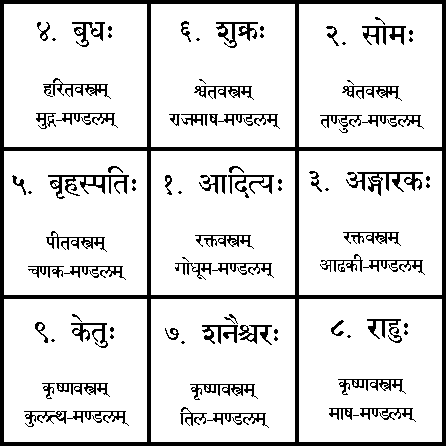
\includegraphics{purvanga/navagraha-diagram.pdf}

\twolineshloka
{जपाकुसुमसङ्काशं काश्यपेयं महद्युतिम्}
{तमोऽरिं सर्वपापघ्नं प्रणतोऽस्मि दिवाकरम्}

आ स॒त्येन॒ रज॑सा॒ वर्त॑मानो निवे॒शय॑न्न॒मृतं॒ मर्त्यं॑ च। हि॒र॒ण्यये॑न सवि॒ता रथे॒नाऽदे॒वो या॑ति॒
भुव॑ना वि॒पश्य\sn{}। अ॒ग्निं दू॒तं वृ॑णीमहे॒ होता॑रं वि॒श्ववे॑दसम्। अ॒स्य य॒ज्ञस्य॑ सु॒क्रतुम्॥
येषा॒मीशे॑ पशु॒पति॑ पशू॒नां चतु॑ष्पदामु॒त च॑ द्वि॒पदाम्। निष्क्री॑तो॒ऽयं य॒ज्ञियं॑ भा॒गमे॑तु
रा॒यस्पोषा॒ यज॑मानस्य सन्तु॥  अधिदेवता प्रत्यधिदेवता सहिताय आदित्याय॒ नम॥ 

अस्मिन् मण्डले अधिदेवता-प्रत्यधिदेवता-सहितं आदित्य-ग्रहं ध्यायामि। आवाहयामि।

\twolineshloka
{दधिशङ्खतुषाराभं क्षीरोदार्णवसम्भवम्}
{नमामि शशिनं सोमं शम्भोर्मुकुटभूषणम्}

आप्या॑यस्व॒ समे॑तु ते वि॒श्वत॑ सोम॒ वृष्णि॑यम्। भवा॒ वाज॑स्य सङ्ग॒थे॥ अ॒प्सु मे॒ सोमो॑
अब्रवीद॒न्तर्विश्वा॑नि भेष॒जा। अ॒ग्निं च॑ वि॒श्वश॑म्भुव॒माप॑श्च वि॒श्वभे॑षजीः। गौ॒री मि॑माय
सलि॒लानि॒ तक्ष॒ती। एक॑पदी द्वि॒पदी॒ सा चतु॑ष्पदी। अ॒ष्टाप॑दी॒ नव॑पदी बभू॒वुषी। स॒हस्राक्षरा पर॒मे
व्यो॑मन्।  अधिदेवता प्रत्यधिदेवता सहिताय सोमाय॒ नम॥ 

अस्मिन् मण्डले अधिदेवता-प्रत्यधिदेवता-सहितं सोम-ग्रहं ध्यायामि। आवाहयामि।


\twolineshloka
{धरणीगर्भसम्भूतं विद्युत्कान्तिसमप्रभम्}
{कुमारं शक्तिहस्तं च मङ्गलं प्रणमाम्यहम्}

अ॒ग्निर्मू॒र्द्धा दि॒वः क॒कुत्पति॑ पृथि॒व्या अ॒यम्। अ॒पा रेतासि जिन्वति। स्यो॒ना पृ॑थिवि॒
भवा॑ऽनृक्ष॒रा नि॒वेश॑नी। यच्छा॑न॒ शर्म॑ स॒प्रथा। क्षेत्र॑स्य॒ पति॑ना व॒य हि॒ते ने॑व जयामसि।
गामश्वं॑ पोषयि॒त्न्वा स नो॑ मृडाती॒दृशे॥  अधिदेवता प्रत्यधिदेवता सहिताय अङ्गारकाय॒ नम॥ 

अस्मिन् मण्डले अधिदेवता-प्रत्यधिदेवता-सहितं अङ्गारक-ग्रहं ध्यायामि। आवाहयामि।


\twolineshloka
{प्रियङ्गुकलिकाश्यामं रूपेणाप्रतिमं बुधम्}
{सौम्यं सौम्यगुणोपेतं तं बुधं प्रणमाम्यहम्}

उद्बु॑ध्यस्वाग्ने॒ प्रति॑जागृह्येनमिष्टापू॒र्ते ससृ॑जेथाम॒यं च॑। पुन॑ कृ॒ण्वस्त्वा॑ पि॒तरं॒
युवा॑नम॒न्वातासी॒त्वयि॒ तन्तु॑मे॒तम्॥ इ॒दं विष्णु॒र्विच॑क्रमे त्रे॒धा निद॑धे प॒दम्। समू॑ढमस्यपा
सु॒रे॥ विष्णो॑ र॒राट॑मसि॒ विष्णो पृ॒ष्ठम॑सि॒ विष्णो॒ श्नप्त्रेस्थो॒ विष्णो॒ स्यूर॑सि॒
विष्णोर्ध्रु॒वम॑सि वैष्ण॒वम॑सि॒ विष्ण॑वे त्वा।  अधिदेवता प्रत्यधिदेवता सहिताय बुधाय॒ नम॥ 

अस्मिन् मण्डले अधिदेवता-प्रत्यधिदेवता-सहितं बुध-ग्रहं ध्यायामि। आवाहयामि।


\twolineshloka
{देवानां च ऋषीणां च गुरुं काञ्चनसन्निभम्}
{बुद्धिभूतं त्रिलोकेशं तं नमामि बृहस्पतिम्}

बृह॑स्पते॒ अति॒यद॒र्यो अर्हाद्वि॒मद्वि॒भाति॒ क्रतु॑म॒ज्जने॑षु। यद्दी॒दय॒च्छव॑सर्त\-प्रजात॒
तद॒स्मासु॒ द्रवि॑णं धेहि चि॒त्रम्॥ इन्द्र॑मरुत्व इ॒ह पा॑हि॒ सोमं॒ यथा॑ शार्या॒ते अपि॑बः सु॒तस्य॑।
तव॒ प्रणी॑ती॒ तव॑ शूर॒शर्म॒न्नावि॑वासन्ति क॒वय॑ सुय॒ज्ञाः॥ ब्रह्म॑जज्ञा॒नं प्र॑थ॒मं
पु॒रस्ता॒द्विसी॑म॒तः सु॒रुचो॑ वे॒न आ॑वः। सबु॒ध्निया॑ उप॒मा अ॑स्य वि॒ष्ठाः स॒तश्च॒ योनि॒मस॑तश्च॒
विव॑॥ अधिदेवता प्रत्यधिदेवता सहिताय बृहस्पतये॒ नम॥ 

अस्मिन् मण्डले अधिदेवता-प्रत्यधिदेवता-सहितं बृहस्पति-ग्रहं ध्यायामि। आवाहयामि।

\twolineshloka
{हिमकुन्दमृणालाभं दैत्यानां परमं गुरुम्}
{सर्वशास्त्रप्रवक्तारं भार्गवं प्रणमाम्यहम्}

प्रव॑ शु॒क्राय॑ भा॒नवे॑ भरध्व ह॒व्यं म॒तिं चा॒ग्नये॒ सुपू॑तम्॥ यो दैव्या॑नि॒ मानु॑षा
ज॒नूष्य॒न्तर्विश्वा॑नि वि॒द्म ना॒ जिगा॑ति॥ इ॒न्द्रा॒णीमा॒सु नारि॑षु सु॒पत्नी॑म॒हम॑श्रवम्। न
ह्य॑स्या अप॒रञ्च॒न ज॒रसा॒ मर॑ते॒ पति॑॥ इन्द्रं॑ वो वि॒श्वत॒स्परि॒ हवा॑महे॒ जनेभ्यः। अ॒स्माक॑मस्तु॒
केव॑लः॥  अधिदेवता प्रत्यधिदेवता सहिताय शुक्राय॒ नम॥ 

अस्मिन् मण्डले अधिदेवता-प्रत्यधिदेवता-सहितं शुक्र-ग्रहं ध्यायामि। आवाहयामि।

\twolineshloka
{नीलाञ्जनसमाभासं रविपुत्रं यमाग्रजम्}
{छायामार्तण्डसम्भूतं तं नमामि शनैश्चरम्}

शं नो॑ दे॒वीर॒भिष्ट॑य॒ आपो॑ भवन्तु पी॒तये। शंयोर॒भिस्र॑वन्तु नः॥ प्रजा॑पते॒ न त्वदे॒तान्य॒न्यो
विश्वा॑ जा॒तानि॒ परि॒ता ब॑भूव। यत्का॑मास्ते जुहु॒मस्तन्नो॑ अस्तु व॒य स्या॑म॒ पत॑यो रयी॒णाम्। इ॒मं
य॑मप्रस्त॒रमाहि सीदाऽङ्गि॑रोभिः पि॒तृभि॑ संविदा॒नः। आत्वा॒ मन्त्रा कविश॒स्ता व॑हन्त्वे॒ना रा॑जन्
ह॒विषा॑ मादयस्व॥  अधिदेवता प्रत्यधिदेवता सहिताय शनैश्चराय॒ नम॥ 

अस्मिन् मण्डले अधिदेवता-प्रत्यधिदेवता-सहितं शनैश्चर-ग्रहं ध्यायामि। आवाहयामि।

\twolineshloka
{अर्धकायं महावीर्यं चन्द्रादित्यविमर्दनम्}
{सिंहिकागर्भसम्भूतं तं राहुं प्रणमाम्यहम्}

कया॑ नश्चि॒त्र आभु॑वदू॒ती स॒दावृ॑ध॒ सखा। कया॒ शचि॑ष्ठया वृ॒ता। आऽयङ्गौः
पृश्नि॑रक्रमी॒दस॑नन्मा॒तरं॒ पुन॑। पि॒तरं॑ च प्र॒यन्त्सुव॑। यत्ते॑ दे॒वी निर्ऋ॑तिराब॒बन्ध॒ दाम॑
ग्री॒वास्व॑विच॒र्त्यम्। इ॒दं  ते॒ तद्विष्या॒म्यायु॑षो॒ न मध्या॒दथा॑जी॒वः पि॒तुम॑द्धि॒ प्रमु॑क्तः॥ 
अधिदेवता प्रत्यधिदेवता सहिताय राहवे॒ नम॥ 

अस्मिन् मण्डले अधिदेवता-प्रत्यधिदेवता-सहितं राहु-ग्रहं ध्यायामि। आवाहयामि।

\twolineshloka
{पलाशपुष्पसङ्काशं तारकाग्रहमस्तकम्}
{रौद्रं रौद्रात्मकं घोरं तं केतुं प्रणमाम्यहम्}

के॒तुं कृ॒ण्वन्न॑के॒तवे॒ पेशो॑ मर्या अपे॒शसे। समु॒षद्भि॑रजायथाः॥ ब्र॒ह्मा दे॒वानां पद॒वीः
क॑वी॒नामृषि॒र्विप्रा॑णां महि॒षो मृ॒गाणाम्। श्ये॒नो गृध्रा॑णा॒ स्वधि॑ति॒र्वना॑ना॒ सोम॑
प॒वित्र॒मत्ये॑ति॒ रेभ\sn{}। (ऋक्) सचि॑त्र चि॒त्रं चि॒तयन् तम॒स्मे चित्र॑क्षत्र चि॒त्रत॑मं वयो॒धाम्।
च॒न्द्रं र॒यिं पु॑रु॒वीरं बृ॒हन्तं॒ चन्द्र॑च॒न्द्राभि॑र्गृण॒ते यु॑वस्व॥  अधिदेवता प्रत्यधिदेवता
सहिताय केतवे॒ नम॥ 

अस्मिन् मण्डले अधिदेवता-प्रत्यधिदेवता-सहितं केतु-ग्रहं ध्यायामि। आवाहयामि।

आदित्यादि नवग्रहदेवताभ्यो नमः आसनं समर्पयामि।
पाद्यं समर्पयामि। अर्घ्यं समर्पयामि। आचमनीयं समर्पयामि। 

शुद्धोदकस्नानं समर्पयामि। स्नानानन्तरम् आचमनीयं समर्पयामि।
वस्त्रार्थम् अक्षतान् समर्पयामि।\\
यज्ञोपवीताभरणार्थे अक्षतान् समर्पयामि।\\
दिव्यपरिमलगन्धान् धारयामि।\\
गन्धस्योपरि हरिद्राकुङ्कुमं समर्पयामि। अक्षतान् समर्पयामि। \\
पुष्पैः पूजयामि।

\begin{enumerate}%[label=\devanumber\value{enumi}]
\item ॐ आदित्याय नमः
\item ॐ अङ्गारकाय नम​:
\item ॐ शुक्राय नमः
\item ॐ सोमाय नम​:
\item ॐ बुधाय नम​:
\item ॐ बृहस्पतये नमः
\item ॐ शनैश्चराय नमः
\item ॐ राहवे नमः
\item ॐ केतवे नम​:
\end{enumerate}

नानाविध-परिमल-पत्र-पुष्पाणि समर्पयामि।

आदित्यादि नवग्रहदेवताभ्यो नमः धूपमाघ्रापयामि।\\
दीपं दर्शयामि।\\
नैवेद्यम्। \\
कर्पूरताम्बूलं समर्पयामि। कर्पूरनीराजनं दर्शयामि।\\
प्रार्थनाः समर्पयामि।
अनन्तकोटिप्रदक्षिणनमस्कारान् समर्पयामि।\\

आदित्यादि नवग्रहदेवताभ्यो नमः (अक्षतान् समर्पयित्वा) यथास्थानं प्रतिष्ठापयामि। शोभनार्थे क्षेमाय पुनरागमनाय च।


% !TeX program = XeLaTeX
% !TeX root = ..\pujavidhanam.tex

\sect{लोकपालपूजा}

प्राणान् आयम्य। ममोपात्तसमस्तदुरितक्षयद्वारा श्रीपरमेश्वरप्रीत्यर्थम् अद्य-पूर्वोक्त एवं गुण-विशेषेण विशिष्टायाम् अस्यां
अमावास्यायां शुभतिथौ श्रीमहालक्ष्मी-पूजाङ्गभूतां ब्रह्म-विष्णु-त्र्यम्बक-क्षेत्रपाल-पूजां करिष्ये।

अस्मिन् कूर्चे ब्रह्मादीन् ध्यायामि। ब्रह्मन् सरस्वत्या सह इह आगच्छ आगच्छ। सरस्वती-सहित-ब्रह्माणम् आवाहयामि। आसनं समर्पयामि।

लक्ष्मी-विष्णुभ्यां नमः।\\
ध्यायामि। आवाहयामि। आसनं समर्पयामि।

दुर्गा-त्र्यम्बकाभ्यां नमः।\\
ध्यायामि। आवाहयामि। आसनं समर्पयामि।

क्षेत्रपाल-भूमिभ्यां नमः।\\
ध्यायामि। आवाहयामि। आसनं समर्पयामि।

ब्रह्मादिभ्यो नमः पाद्यं समर्पयामि। अर्घ्यं समर्पयामि।
आचमनीयं समर्पयामि। शुद्धोदकस्नानं समर्पयामि। स्नानानन्तरम् आचमनीयं समर्पयामि।
वस्त्रार्थम् अक्षतान् समर्पयामि।
यज्ञोपवीताभरणार्थे अक्षतान् समर्पयामि।
दिव्यपरिमलगन्धान् धारयामि।
गन्धस्योपरि हरिद्राकुङ्कुमं समर्पयामि। अक्षतान् समर्पयामि। \\
पुष्पैः पूजयामि।\\

नैवेद्यम्। \\
कर्पूरताम्बूलं समर्पयामि। कर्पूरनीराजनं दर्शयामि।\\
प्रार्थनाः समर्पयामि।
अनन्तकोटिप्रदक्षिणनमस्कारान् समर्पयामि।\\

ब्रह्मादिभ्यो नमः (अक्षतान् समर्पयित्वा) यथास्थानं प्रतिष्ठापयामि। शोभनार्थे क्षेमाय पुनरागमनाय च।

\dnsub{प्रार्थना}

\twolineshloka*
{विघ्नराजं नमस्कृत्य नमस्कृत्य विधिं परम्}
{विष्णुं रुद्रं श्रियं दुर्गां वन्दे भक्त्या सरस्वतीम्}

\twolineshloka*
{क्षेत्राधिपं नमस्कृत्य दिवानाथं निशाकरम्}
{धरणीगर्भसम्भूतं शशिपुत्रं बृहस्पतिम्}

\twolineshloka*
{दैत्याचार्यं नमस्कृत्य सूर्यपुत्रं महाग्रहम्}
{राहुकेतू नमस्कृत्य यज्ञारम्भे विशेषतः}

\twolineshloka*
{शक्राद्या देवताः सर्वाः मुनींश्च प्रणमाम्यहम्}
{गर्गं मुनिं नमस्कृत्य नारदं मुनिसत्तमम्}

\twolineshloka*
{वसिष्ठं मुनिशार्दूलं विश्वामित्रं भृगोः सुतम्}
{व्यासं मुनिं नमस्कृत्य आचार्यांश्च तपोधनान्}

\twolineshloka*
{सर्वान् तान् प्रणमाम्येवं यज्ञरक्षाकरान् सदा}
{शङ्खचक्रगदाशार्ङ्ग-पद्मपाणिर्जनार्दनः}
\onelineshloka*
{सर्वासु दिक्षु रक्षेन्मां यावत् पूजावसानकम्}


\sect{षोडशोपचारपूजा}
\begin{center}
\fourlineindentedshloka*
{अरुणकमलसंस्था तद्रजःपुञ्जवर्णा}
{करकमलधृतेष्टाऽभीतियुग्माम्बुजा च}
{मणिमकुटविचित्रालङ्कृता कल्पजातैः}
{भवतु भुवनमाता सन्ततं श्रीः श्रियै नः}

अस्मिन् बिम्बे श्रीमहालक्ष्मीं ध्यायामि।

\twolineshloka*
{आवाहये महालक्ष्मि चैतन्यस्तन्यदायिनि}
{विष्णुपत्नि जगन्मातः पूजां गृह्णीष्व ते नमः}
श्रीमहालक्ष्मीम् आवाहयामि।

\twolineshloka*
{तप्तकाञ्चनवर्णाभं मुक्तामणिविराजितम्}
{अमलं कमलं दिव्यम् आसनं प्रतिगृह्यताम्}
 आसनं समर्पयामि।\medskip


\twolineshloka*
{गङ्गातीर्थ-समुद्भूतं गन्ध-पुष्पादिभिर्युतम्}
{पाद्यं ददाम्यहं देवि गृहाणाऽऽशु नमोऽस्तु ते}
 पाद्यं समर्पयामि।\medskip

\twolineshloka*
{एलागन्धसमायुक्तं स्वर्णपात्रे प्रपूरितम्}
{अर्घ्यं गृहाण मद्दत्तं प्रसीद त्वं महेश्वरि}
 अर्घ्यं समर्पयामि।\medskip


\twolineshloka*
{सर्वलोकस्य या शक्तिः ब्रह्मरुद्रादिभिः स्तुता}
{ददाम्याचमनं तस्यै महालक्ष्म्यै मनोहरम्}
 आचमनीयं समर्पयामि।\medskip

घृतेन स्नपयामि। पुनः शुद्धोदकं समर्पयामि।\\
पयसा स्नपयामि। पुनः शुद्धोदकं समर्पयामि।\\
दध्ना स्नपयामि। पुनः शुद्धोदकं समर्पयामि।\\
मधुना स्नपयामि। पुनः शुद्धोदकं समर्पयामि।\\
पञ्चामृतेन स्नपयामि। पुनः शुद्धोदकं समर्पयामि।

(कलशजलेन श्री-सूक्तं जप्य) शुद्धोदकस्नानं समर्पयामि।
स्नानानन्तरम् आचमनीयं समर्पयामि।\medskip

\twolineshloka*
{दिव्याम्बरयुगं सूक्ष्मं कञ्चुकं च मनोहरम्}
{महालक्ष्मि महादेवि गृहाणेदं मयाऽर्पितम्}
 वस्त्रं समर्पयामि।\medskip

\twolineshloka*
{माङ्गल्यमणिसंयुक्तं मुक्ताविद्रुमसंयुतम्}
{दत्तं मङ्गलसूत्रं च गृहाण हरिवल्लभे}
कण्ठसूत्रं समर्पयामि।\medskip


\twolineshloka*
{रत्नकङ्कणवैडूर्य-मुक्ताहारादिकानि च}
{सुप्रसन्नेन मनसा दत्तानि त्वं गृहाण मे}
आभरणानि समर्पयामि।\medskip

\twolineshloka*
{सिन्दूरारुणवर्णा च सिन्दूरतिलकप्रिया}
{अतो दत्तं मया देवि सिन्दूरं प्रतिगृह्यताम्}
 तिलकं समर्पयामि। \medskip

\twolineshloka*
{मन्दार-पारिजाताद्याः पाटली केतकी तथा}
{माकन्दं कुरवं चैव गृहाणाऽऽशु नमोऽस्तु ते}
  पुष्पमालां धारयामि। 
\end{center}
\dnsub{अङ्गपूजा}
\begin{longtable}{ll@{— }l}
१.& ॐ चपलायै नमः & पादौ पूजयामि \\
२.& चञ्चलायै नमः & जानुनी पूजयामि\\
३.& कमलायै नमः & कटिं पूजयामि  \\
४.& कात्यायन्यै नमः & नाभिं पूजयामि\\
५.& जगन्मात्रे नमः & जठरं पूजयामि   \\
६.& विश्ववल्लभायै नमः & वक्षःस्थलं पूजयामि \\
७.& कमलवासिन्यै नमः & हस्तौ पूजयामि        \\
८.& पद्माननायै नमः & मुखं पूजयामि\\
९.& कमलपत्राक्ष्यै नमः & नेत्रत्रयं पूजयामि    \\
१०.& श्रियै नमः & शिरः पुजयामि\\
११.& महालक्ष्म्यै नमः & सर्वाणि अङ्गानि पूजयामि   \\
\end{longtable}

\dnsub{अष्टलक्ष्मी-अर्चना}
(प्राच्याम् आरभ्य अष्टदिक्षु प्रदक्षिणेन)

\begin{multicols}{2}
\begin{enumerate}
\item ॐ आद्यलक्ष्म्यै नमः
\item ॐ विद्यालक्ष्म्यै नमः
\item ॐ सौभाग्यलक्ष्म्यै नमः
\item ॐ अमृतलक्ष्म्यै नमः
\item ॐ कामलक्ष्म्यै नमः 
\item ॐ सत्यलक्ष्म्यै नमः
\item ॐ भोगलक्ष्म्यै नमः
\item ॐ योगलक्ष्म्यै नमः
\end{enumerate}
\end{multicols}

आद्यादिलक्ष्मीनां षोडशोपचारपूजार्थे पुष्पाणि समर्पयामि।

\dnsub{लक्ष्म्यष्टोत्तरशतनामावलिः}
\begin{multicols}{2}
\begin{flushleft}
ॐ प्रकृत्यै~नमः\\
ॐ विकृत्यै~नमः\\
ॐ विद्यायै~नमः\\
ॐ सर्वभूतहितप्रदायै~नमः\\
ॐ श्रद्धायै~नमः\\
ॐ विभूत्यै~नमः\\
ॐ सुरभ्यै~नमः\\
ॐ परमात्मिकायै~नमः\\
ॐ वाचे~नमः\\
ॐ पद्मालयायै~नमः\hfill\devanumber{10}\\
ॐ पद्मायै~नमः\\
ॐ शुचये~नमः\\
ॐ स्वाहायै~नमः\\
ॐ स्वधायै~नमः\\
ॐ सुधायै~नमः\\
ॐ धन्यायै~नमः\\
ॐ हिरण्मय्यै~नमः\\
ॐ लक्ष्म्यै~नमः\\
ॐ नित्यपुष्टायै~नमः\\
ॐ विभावर्यै~नमः\hfill\devanumber{20}\\
ॐ अदित्यै~नमः\\
ॐ दित्यै~नमः\\
ॐ दीप्तायै~नमः\\
ॐ वसुधायै~नमः\\
ॐ वसुधारिण्यै~नमः\\
ॐ कमलायै~नमः\\
ॐ कान्तायै~नमः\\
ॐ कामायै~नमः\\
ॐ क्षीरोदसम्भवायै~नमः\\
ॐ अनुग्रहपदायै~नमः\hfill\devanumber{30}\\
ॐ बुद्धये~नमः\\
ॐ अनघायै~नमः\\
ॐ हरिवल्लभायै~नमः\\
ॐ अशोकाममृतायै~नमः\\
ॐ दीप्तायै~नमः\\
ॐ लोकशोकविनाशिन्यै~नमः\\
ॐ धर्मनिलयायै~नमः\\
ॐ करुणायै~नमः\\
ॐ लोकमात्रे~नमः\\
ॐ पद्मप्रियायै~नमः\hfill\devanumber{40}\\
ॐ पद्महस्तायै~नमः\\
ॐ पद्माक्ष्यै~नमः\\
ॐ पद्मसुन्दर्यै~नमः\\
ॐ पद्मोद्भवायै~नमः\\
ॐ पद्ममुख्यै~नमः\\
ॐ पद्मनाभप्रियायै~नमः\\
ॐ रमायै~नमः\\
ॐ पद्ममालाधरायै~नमः\\
ॐ देव्यै~नमः\\
ॐ पद्मिन्यै~नमः\hfill\devanumber{50}\\
ॐ पद्मगन्धिन्यै~नमः\\
ॐ पुण्यगन्धायै~नमः\\
ॐ सुप्रसन्नायै~नमः\\
ॐ प्रसादाभिमुख्यै~नमः\\
ॐ प्रभायै~नमः\\
ॐ चन्द्रवदनायै~नमः\\
ॐ चन्द्रायै~नमः\\
ॐ चन्द्रसहोदर्यै~नमः\\
ॐ चतुर्भुजायै~नमः\\
ॐ चन्द्ररूपायै~नमः\hfill\devanumber{60}\\
ॐ इन्दिरायै~नमः\\
ॐ इन्दुशीतलायै~नमः\\
ॐ आह्लादजनन्यै~नमः\\
ॐ पुष्ट्यै~नमः\\
ॐ शिवायै~नमः\\
ॐ शिवकर्यै~नमः\\
ॐ सत्यै~नमः\\
ॐ विमलायै~नमः\\
ॐ विश्वजनन्यै~नमः\\
ॐ तुष्ट्यै~नमः\hfill\devanumber{70}\\
ॐ दारिद्र्यनाशिन्यै~नमः\\
ॐ प्रीतिपुष्करिण्यै~नमः\\
ॐ शान्तायै~नमः\\
ॐ शुक्लमाल्याम्बरायै~नमः\\
ॐ श्रियै~नमः\\
ॐ भास्कर्यै~नमः\\
ॐ बिल्वनिलयायै~नमः\\
ॐ वरारोहायै~नमः\\
ॐ यशस्विन्यै~नमः\\
ॐ वसुन्धरायै~नमः\hfill\devanumber{80}\\
ॐ उदाराङ्गायै~नमः\\
ॐ हरिण्यै~नमः\\
ॐ हेममालिन्यै~नमः\\
ॐ धनधान्यकर्यै~नमः\\
ॐ सिद्ध्यै~नमः\\
ॐ स्त्रैणसौम्यायै~नमः\\
ॐ शुभप्रदायै~नमः\\
ॐ नृपवेश्मगतानन्दायै~नमः\\
ॐ वरलक्ष्म्यै~नमः\\
ॐ वसुप्रदायै~नमः\hfill\devanumber{90}\\
ॐ शुभायै~नमः\\
ॐ हिरण्यप्राकारायै~नमः\\
ॐ समुद्रतनयायै~नमः\\
ॐ जयायै~नमः\\
ॐ मङ्गलायै~नमः\\
ॐ देव्यै~नमः\\
ॐ~विष्णुवक्षःस्थल\-स्थितायै~नमः\\
ॐ विष्णुपत्न्यै~नमः\\
ॐ प्रसन्नाक्ष्यै~नमः\\
ॐ नारायणसमाश्रितायै~नमः\hfill\devanumber{100}\\
ॐ दारिद्र्यध्वंसिन्यै~नमः\\
ॐ देव्यै~नमः\\
ॐ सर्वोपद्रवहारिण्यै~नमः\\
ॐ नवदुर्गायै~नमः\\
ॐ महाकाल्यै~नमः\\
ॐ~ब्रह्मविष्णुशिवात्मिकायै नमः\\
ॐ त्रिकालज्ञानसम्पन्नायै~नमः\\
ॐ भुवनेश्वर्यै~नमः\\
\end{flushleft}
\end{multicols}

\sect{उत्तराङ्गपूजा}

\begin{center}

\twolineshloka*
{वनस्पति-रसोत्पन्नो गन्धाढ्यो गन्ध उत्तमः}
{आघ्रेयः सर्वदेवानां धूपोऽयं प्रतिगृह्यताम्}
श्री महालक्ष्म्यै नमः धूपमाघ्रापयामि।\\
 
\twolineshloka*
{कार्पासवर्तिसंयुक्तं घृतयुक्तं मनोहरम्}
{तमोनाशकरं दीपं गृहाण परमेश्वर}
श्री महालक्ष्म्यै नमः अलङ्कारदीपं सन्दर्शयामि।\\

\twolineshloka*
{नैवेद्यं गृह्यतां लक्ष्मि भक्ष्य-भोज्य-समन्वितम्}
{षड्रसैर्रचितं दिव्यं लक्ष्मीदेवि नमोऽस्तु ते}
नैवेद्यम्\\
- श्री महालक्ष्म्यै नमः (	) निवेदयामि, \\
अमृतापिधानमसि। निवेदनानन्तरम् आचमनीयं समर्पयामि।\\

पूगीफलसमायुक्तं नागवल्लीदलैर्युतम्।\\
कर्पूरचूर्णसंयुक्तं ताम्बूलं प्रतिगृह्यताम्॥\\
श्री महालक्ष्म्यै नमः कर्पूरताम्बूलं समर्पयामि।\\

श्री महालक्ष्म्यै नमः समस्त अपराध क्षमापनार्थं कर्पूरनीराजनं दर्शयामि।\\
कर्पूरनीरजनानन्तरम् आचमनीयं समर्पयामि।\\

 यो॑ऽपां पुष्पं॒ वेद॑। पुष्प॑वान् प्र॒जावान् पशु॒मान् भ॑वति।\\
च॒न्द्रमा॒ वा अ॒पां पुष्पम्। पुष्प॑वान् प्र॒जावान् पशु॒मान् भ॑वति।\\
य ए॒वं वेद॑। यो॑ऽपामा॒यत॑नं॒ वेद॑। आ॒यत॑नवान् भवति।\\

ओं तद्ब्र॒ह्म। ओं तद्वा॒युः। ओं तदा॒त्मा। ओं᳚ तथ्स॒त्यम्‌।\\
ओं᳚ तथ्सर्वम्᳚‌। ओं तत्पुरो॒र्नमः॥\\

अन्तश्चरति॑ भूते॒षु॒ गुहायां वि॑श्वमू॒र्तिषु। \\
त्वं यज्ञस्त्वं वषट्कारस्त्वमिन्द्रस्त्व रुद्रस्त्वं विष्णुस्त्वं ब्रह्म त्वं॑ प्रजा॒पतिः। \\
त्वं त॑दाप॒ आपो॒ ज्योती॒ रसो॒ऽमृतं॒ ब्रह्म॒ भूर्भुव॒स्सुव॒रोम्‌॥\\

श्री महालक्ष्म्यै नमः वेदोक्तमन्त्रपुष्पाञ्जलिं समर्पयामि।\\

स्वर्णपुष्पं समर्पयामि\\
 
अनन्तकोटिप्रदक्षिणनमस्कारान् समर्पयामि\\

छत्त्रचामरादिसमस्तोपचारान् समर्पयामि\\

हिरण्यगर्भगर्भस्थं हेमबीजं विभावसोः।\\
अनन्तपुण्यफलदम् अतः शान्तिं प्रयच्छ मे॥\\

आश्वयुज-अमावास्या-पुण्यकालेऽस्मिन् मया क्रियमाण श्री\-महा\-लक्ष्मी-पूजायां
यद्देयमुपायन\-दानं तत्प्रति\-निधित्वेन हिरण्यं श्री महा\-लक्ष्मी\-प्रीतिं
कामयमानः मनसोद्दिष्टाय ब्राह्मणाय सम्प्रददे नमः न मम। 
अनया पूजया श्री महालक्ष्मीः प्रीयताम्। 
\end{center}

\sect{ईशानादि पूजा}

\sect{कुबेर पूजा}



\dnsub{कुबेराष्टोत्तरशतनामावलिः}

\fourlineindentedshloka*
{मनुजबाह्यविमानवरस्तुतम्}
{गरुडरत्ननिभं निधिनायकम्}
{शिवसखं मुकुटादिविभूषितम्}
{वररुचिं तमहमुपास्महे सदा}

\twolineshloka*
{अगस्त्य देवदेवेश मर्त्यलोकहितेच्छया}
{पूजयामि विधानेन प्रसन्नसुमुखो भव}
\begin{multicols}{2}
\begin{flushleft}
ॐ कुबेराय नमः\\
ॐ धनदाय नमः\\
ॐ श्रीमते नमः\\
ॐ यक्षेशाय नमः\\
ॐ गुह्यकेश्वराय नमः\\
ॐ निधीशाय नमः\\
ॐ शङ्करसखाय नमः\\
ॐ महालक्ष्मीनिवासभुवे नमः\\
ॐ महापद्मनिधीशाय नमः\\
ॐ पूर्णाय नमः\hfill\devanumber{10}\\ %१०
ॐ पद्मनिधीश्वराय नमः\\
ॐ शङ्खाख्यनिधिनाथाय नमः\\
ॐ मकराख्यनिधिप्रियाय नमः\\
ॐ सुकच्छपाख्यनिधीशाय नमः\\
ॐ मुकुन्दनिधिनायकाय नमः\\
ॐ कुन्दाख्यनिधिनाथाय नमः\\
ॐ नीलनित्याधिपाय नमः\\
ॐ महते नमः\\
ॐ वरनिधिदीपाय नमः\\
ॐ पूज्याय नमः\hfill\devanumber{20}\\ %२०
ॐ लक्ष्मीसाम्राज्यदायकाय नमः\\
ॐ इलपिलापत्याय नमः\\
ॐ कोशाधीशाय नमः\\
ॐ कुलोचिताय नमः\\
ॐ अश्वारूढाय नमः\\
ॐ विश्ववन्द्याय नमः\\
ॐ विशेषज्ञाय नमः\\
ॐ विशारदाय नमः\\
ॐ नलकूबरनाथाय नमः\\
ॐ मणिग्रीवपित्रे नमः\hfill\devanumber{30}\\ %३०
ॐ गूढमन्त्राय नमः\\
ॐ वैश्रवणाय नमः\\
ॐ चित्रलेखामनःप्रियाय नमः\\
ॐ एकपिनाकाय नमः\\
ॐ अलकाधीशाय नमः\\
ॐ पौलस्त्याय नमः\\
ॐ नरवाहनाय नमः\\
ॐ कैलासशैलनिलयाय नमः\\
ॐ राज्यदाय नमः\\
ॐ रावणाग्रजाय नमः\hfill\devanumber{40}\\ %४०
ॐ चित्रचैत्ररथाय नमः\\
ॐ उद्यानविहाराय नमः\\
ॐ विहारसुकुतूहलाय नमः\\
ॐ महोत्सहाय नमः\\
ॐ महाप्राज्ञाय नमः\\
ॐ सदापुष्पकवाहनाय नमः\\
ॐ सार्वभौमाय नमः\\
ॐ अङ्गनाथाय नमः\\
ॐ सोमाय नमः\\
ॐ सौम्यादिकेश्वराय नमः\hfill\devanumber{50}\\ %५०
ॐ पुण्यात्मने नमः\\
ॐ पुरुहुतश्रियै नमः\\
ॐ सर्वपुण्यजनेश्वराय नमः\\
ॐ नित्यकीर्तये नमः\\
ॐ निधिवेत्रे नमः\\
ॐ लङ्काप्राक्तननायकाय नमः\\
ॐ यक्षिणीवृताय नमः\\
ॐ यक्षाय नमः\\
ॐ परमशान्तात्मने नमः\\
ॐ यक्षराजे नमः\hfill\devanumber{60}\\ %६०
ॐ यक्षिणीहृदयाय नमः\\ 
ॐ किन्नरेश्वराय नमः\\
ॐ किम्पुरुषनाथाय नमः\\
ॐ खड्गायुधाय नमः\\
ॐ वशिने नमः\\
ॐ ईशानदक्षपार्श्वस्थाय नमः\\
ॐ वायुवामसमाश्रयाय नमः\\
ॐ धर्ममार्गनिरताय नमः\\
ॐ धर्मसम्मुखसंस्थिताय नमः\\
ॐ नित्येश्वराय नमः\hfill\devanumber{70}\\ %७०
ॐ धनाध्यक्षाय नमः\\
ॐ अष्टलक्ष्म्याश्रितालयाय नमः\\
ॐ मनुष्यधर्मिणे नमः\\
ॐ सुकृतिने नमः\\
ॐ कोषलक्ष्मीसमाश्रिताय नमः\\
ॐ धनलक्ष्मीनित्यवासाय नमः\\
ॐ धान्यलक्ष्मीनिवासभुवे नमः\\
ॐ अष्टलक्ष्मीसदावासाय नमः\\
ॐ गजलक्ष्मीस्थिरालयाय नमः\\
ॐ राज्यलक्ष्मीजन्मगेहाय नमः\hfill\devanumber{80}\\ %८०
ॐ धैर्यलक्ष्मीकृपाश्रयाय नमः\\
ॐ अखण्डैश्वर्यसंयुक्ताय नमः\\
ॐ नित्यानन्दाय नमः\\
ॐ सुखाश्रयाय नमः\\
ॐ नित्यतृप्ताय नमः\\
ॐ निराशाय नमः\\
ॐ निरुपद्रवाय नमः\\
ॐ नित्यकामाय नमः\\
ॐ निराकाङ्क्षाय नमः\\
ॐ निरूपाधिकवासभुवे नमः\hfill\devanumber{90}\\ %९०
ॐ शान्ताय नमः\\
ॐ सर्वगुणोपेताय नमः\\
ॐ सर्वज्ञाय नमः\\
ॐ सर्वसम्मताय नमः\\
ॐ सर्वाणिकरुणापात्राय नमः\\
ॐ सदानन्दकृपालयाय नमः\\
ॐ गन्धर्वकुलसंसेव्याय नमः\\
ॐ सौगन्धिककुसुमप्रियाय नमः\\
ॐ स्वर्णनगरीवासाय नमः\\
ॐ निधिपीठसमाश्रयाय नमः\hfill\devanumber{100}\\ %१००
ॐ महामेरूत्तरस्थाय नमः\\
ॐ महर्षिगणसंस्तुताय नमः\\
ॐ तुष्टाय नमः\\
ॐ शूर्पणखाज्येष्ठाय नमः\\
ॐ शिवपूजारताय नमः\\
ॐ अनघाय नमः\\
ॐ राजयोगसमायुक्ताय नमः\\
ॐ राजशेखरपूज्याय नमः\\
ॐ राजराजाय नमः\\ %१०९
\end{flushleft}
\end{multicols}


\sect{प्रार्थना}
\sect{अपराध-क्षमापनम्}
% !TeX program = XeLaTeX
% !TeX root = ../pujavidhanam.tex

\setlength{\parindent}{0pt}
\chapt{श्री तुलसी-पूजा}

\sect{पूर्वाङ्गविघ्नेश्वरपूजा}

(आचम्य)
\twolineshloka*
{शुक्लाम्बरधरं विष्णुं शशिवर्णं चतुर्भुजम्}
{प्रसन्नवदनं ध्यायेत् सर्वविघ्नोपशान्तये}
 
प्राणान्  आयम्य।  ॐ भूः + भूर्भुवः॒ सुव॒रोम्।
 
(अप उपस्पृश्य, पुष्पाक्षतान् गृहीत्वा)\\
ममोपात्तसमस्त दुरितक्षयद्वारा \\
श्रीपरमेश्वरप्रीत्यर्थं करिष्यमाणस्य कर्मणः\\
 निर्विघ्नेन परिसमाप्त्यर्थम् आदौ विघ्नेश्वरपूजां करिष्ये।

\twolineshloka*
{ॐ ग॒णानां᳚ त्वा ग॒णप॑तिꣳ हवामहे क॒विं क॑वी॒नामु॑प॒मश्र॑वस्तमम्}
{ज्ये॒ष्ठ॒राजं॒ ब्रह्म॑णां ब्रह्मणस्पत॒ आ नः॑ शृ॒ण्वन्नू॒तिभिः॑ सीद॒ साद॑नम्}
अस्मिन् हरिद्राबिम्बे महागणपतिं ध्यायामि, आवाहयामि।\\


ॐ महागणपतये नमः  आसनं समर्पयामि।\\
पादयोः पाद्यं समर्पयामि। हस्तयोरर्घ्यं समर्पयामि।\\
आचमनीयं समर्पयामि।\\
ॐ भूर्भुवस्सुवः। शुद्धोदकस्नानं समर्पयामि।\\
स्नानानन्तरमाचमनीयं समर्पयामि।\\
वस्त्रार्थमक्षतान् समर्पयामि।\\
यज्ञोपवीताभरणार्थे अक्षतान् समर्पयामि।\\
दिव्यपरिमलगन्धान् धारयामि।\\
गन्धस्योपरि हरिद्राकुङ्कुमं समर्पयामि। अक्षतान् समर्पयामि। \\
पुष्पमालिकां समर्पयामि। पुष्पैः पूजयामि।

\dnsub{अर्चना}
% \setenumerate{label=\devanumber.}
% \renewcommand{\labelenumi}{\devanumber\theenumi.}
\begin{enumerate}%[label=\devanumber\value{enumi}]
\begin{minipage}{0.475\linewidth}   
\item ॐ सुमुखाय नमः
\item ॐ एकदन्ताय नमः
\item ॐ कपिलाय नमः
\item ॐ गजकर्णकाय नमः
\item ॐ लम्बोदराय नमः
\item ॐ विकटाय नमः
\item ॐ विघ्नराजाय नमः
\item ॐ विनायकाय नमः
\item ॐ धूमकेतवे नमः
  \end{minipage}
  \begin{minipage}{0.525\linewidth}
\item ॐ गणाध्यक्षाय नमः
\item ॐ फालचन्द्राय नमः
\item ॐ गजाननाय नमः
\item ॐ वक्रतुण्डाय नमः
\item ॐ शूर्पकर्णाय नमः
\item ॐ हेरम्बाय नमः
\item ॐ स्कन्दपूर्वजाय नमः
\item ॐ सिद्धिविनायकाय नमः
\item ॐ विघ्नेश्वराय नमः
  \end{minipage}
\end{enumerate}
नानाविधपरिमलपत्रपुष्पाणि समर्पयामि॥\\
धूपमाघ्रापयामि।\\
अलङ्कारदीपं सन्दर्शयामि।\\
नैवेद्यम्।\\
ताम्बूलं समर्पयामि।\\
कर्पूरनीराजनं समर्पयामि।\\
कर्पूरनीराजनानन्तरमाचमनीयं समर्पयामि।\\
{वक्रतुण्डमहाकाय कोटिसूर्यसमप्रभ।}\\
{अविघ्नं कुरु मे देव सर्वकार्येषु सर्वदा॥}\\
प्रार्थनाः समर्पयामि।

अनन्तकोटिप्रदक्षिणनमस्कारान् समर्पयामि।\\
छत्त्रचामरादिसमस्तोपचारान् समर्पयामि।\\


\sect{प्रधान-पूजा — तुलसी-पूजा}

\twolineshloka*
{शुक्लाम्बरधरं विष्णुं शशिवर्णं चतुर्भुजम्}
{प्रसन्नवदनं ध्यायेत् सर्वविघ्नोपशान्तये}
 
प्राणान्  आयम्य।  ॐ भूः + भूर्भुवः॒ सुव॒रोम्।

\dnsub{सङ्कल्पः}

ममोपात्तसमस्तदुरितक्षयद्वारा श्रीपरमेश्वरप्रीत्यर्थं शुभे शोभने मुहूर्ते अद्यब्रह्मणः
द्वितीयपरार्द्धे श्वेतवराहकल्पे वैवस्वतमन्वन्तरे अष्टाविंशतितमे कलियुगे प्रथमे पादे
जम्बूद्वीपे भारतवर्षे भरतखण्डे मेरोः दक्षिणेपार्श्वे शकाब्दे अस्मिन् वर्तमाने व्यावहारिके
 प्रभवादि षष्टिसंवत्सराणां मध्ये (  )\see{app:samvatsara_names} नाम संवत्सरे दक्षिणायने
शरद-ऋतौ  वृश्चिकमासे शुक्ल पक्षे द्वादश्यां शुभतिथौ
(इन्दु / भौम / बुध / गुरु / भृगु / स्थिर / भानु) वासरयुक्तायाम्
(  )\see{app:nakshatra_names} नक्षत्र (  )\see{app:yoga_names} नाम  योग  (  ) करण युक्तायां च एवं गुण विशेषण विशिष्टायाम्
अस्याम् (एकादश्यां / द्वादश्यां) शुभतिथौ
अस्माकं सहकुटुम्बानां क्षेमस्थैर्य-धैर्य-वीर्य-विजय आयुरारोग्य ऐश्वर्याभिवृद्ध्यर्थम्
 धर्मार्थकाममोक्ष\-चतुर्विधफलपुरुषार्थसिद्ध्यर्थं पुत्रपौत्राभि\-वृद्ध्यर्थम् इष्टकाम्यार्थसिद्ध्यर्थम्
मम इहजन्मनि पूर्वजन्मनि जन्मान्तरे च सम्पादितानां ज्ञानाज्ञानकृतमहा\-पातकचतुष्टय
व्यतिरिक्तानां रहस्यकृतानां प्रकाशकृतानां सर्वेषां पापानां सद्य अपनोदनद्वारा सकल
पापक्षयार्थं श्रीमहाविष्णु-तुलसी-प्रीत्यर्थं यावच्छक्ति ध्यानावाहनादि
षोडशोपचार श्रीमहाविष्णु-तुलसी-पूजां करिष्ये। तदङ्गं कलशपूजां च करिष्ये।


श्रीविघ्नेश्वराय नमः यथास्थानं प्रतिष्ठापयामि।\\
(गणपति प्रसादं शिरसा गृहीत्वा)

\dnsub{आसन-पूजा}
\centerline{पृथिव्या  मेरुपृष्ठ  ऋषिः।  सुतलं  छन्दः।  कूर्मो  देवता॥}
\twolineshloka*
{पृथ्वि  त्वया  धृता  लोका  देवि  त्वं  विष्णुना  धृता}
{त्वं  च  धारय  मां  देवि  पवित्रं  चाऽऽसनं  कुरु}


\dnsub{घण्टापूजा}
\twolineshloka*
{आगमार्थं तु देवानां गमनार्थं तु रक्षसाम्}
{घण्टारवं करोम्यादौ देवताऽऽह्वानकारणम्}


\dnsub{कलशपूजा}
ॐ कलशाय नमः दिव्यगन्धान् धारयामि।\\
ॐ गङ्गायै नमः। ॐ यमुनायै नमः। ॐ गोदावर्यै नमः।  ॐ सरस्वत्यै नमः। ॐ नर्मदायै नमः। ॐ सिन्धवे नमः। ॐ कावेर्यै नमः।\\
ॐ सप्तकोटिमहातीर्थान्यावाहयामि।\\[-0.25ex]

(अथ कलशं स्पृष्ट्वा जपं कुर्यात्) \\
आपो॒ वा इ॒द सर्वं॒ विश्वा॑ भू॒तान्याप॑ प्रा॒णा वा आप॑ प॒शव॒ आपो\-ऽन्न॒मापोऽमृ॑त॒माप॑ स॒म्राडापो॑ वि॒राडाप॑ स्व॒राडाप॒श्\-छन्दा॒स्यापो॒ ज्योती॒ष्यापो॒ यजू॒ष्याप॑ स॒त्यमाप॒ सर्वा॑ दे॒वता॒ आपो॒ भूर्भुव॒ सुव॒राप॒ ओम्॥\\

\twolineshloka* 
{कलशस्य मुखे विष्णुः कण्ठे रुद्रः समाश्रितः}
{मूले तत्र स्थितो ब्रह्मा मध्ये मातृगणाः स्मृताः}
\threelineshloka* 
{कुक्षौ तु सागराः सर्वे सप्तद्वीपा वसुन्धरा}
{ऋग्वेदोऽथ यजुर्वेदः सामवेदोऽप्यथर्वणः}
{अङ्गैश्च सहिताः सर्वे कलशाम्बुसमाश्रिताः}
\twolineshloka* 
{गङ्गे च यमुने चैव गोदावरि सरस्वति}
{नर्मदे सिन्धुकावेरि जलेऽस्मिन् सन्निधिं कुरु}
\twolineshloka*
{सर्वे समुद्राः सरितः तीर्थानि च ह्रदा नदाः}
{आयान्तु देवपूजार्थं दुरितक्षयकारकाः}

\centerline{ॐ भूर्भुवः॒ सुवो॒ भूर्भुवः॒ सुवो॒ भूर्भुवः॒ सुवः॑।}

(इति कलशजलेन सर्वोपकरणानि आत्मानं च प्रोक्ष्य।)


\dnsub{आत्म-पूजा}
ॐ आत्मने नमः, दिव्यगन्धान् धारयामि।
\begin{multicols}{2}
१. ॐ आत्मने नमः\\
२. ॐ अन्तरात्मने नमः\\
३. ॐ योगात्मने नमः\\
४. ॐ जीवात्मने नमः\\
५. ॐ परमात्मने नमः\\
६. ॐ ज्ञानात्मने नमः
\end{multicols}
समस्तोपचारान् समर्पयामि।

\twolineshloka*
{देहो देवालयः प्रोक्तो जीवो देवः सनातनः}
{त्यजेदज्ञाननिर्माल्यं सोऽहं भावेन पूजयेत्}


\begin{minipage}{\linewidth}
\dnsub{पीठ-पूजा}

\begin{multicols}{2}
\begin{enumerate}
\item ॐ आधारशक्त्यै नमः
\item ॐ मूलप्रकृत्यै नमः
\item ॐ आदिकूर्माय नमः 
\item ॐ आदिवराहाय नमः
\item ॐ अनन्ताय नमः
\item ॐ पृथिव्यै नमः
\item ॐ रत्नमण्डपाय नमः
\item ॐ रत्नवेदिकायै नमः
\item ॐ स्वर्णस्तम्भाय नमः
\item ॐ श्वेतच्छत्त्राय नमः
\item ॐ कल्पकवृक्षाय नमः
\item ॐ क्षीरसमुद्राय नमः 
\item ॐ सितचामराभ्यां नमः
\item ॐ योगपीठासनाय नमः
\end{enumerate}
\end{multicols}

\end{minipage}

\dnsub{गुरु ध्यानम्}

\twolineshloka*
{गुरुर्ब्रह्मा गुरुर्विष्णुर्गुरुर्देवो महेश्वरः}
{गुरुः साक्षात् परं ब्रह्म तस्मै श्री गुरवे नमः}


\sect{षोडशोपचारपूजा}
\begin{center}

\twolineshloka*
{ध्यायेच्च तुलसीं देवीं श्यामां कमललोचनाम्}
{प्रसन्नां पद्मकल्हारां वरदाभ्यां चतुर्भुजाम्}

\threelineshloka*
{किरीटहारकेयूरकुण्डलाद्यैर्विभूषिताम्}
{धवलां शुकसंवीतां पद्मासननिषेविताम्}
{देवीं त्रैलोक्यजननीं सर्वलोकैकपावनीम्}
अस्मिन् बिम्बे श्री महाविष्णुं तुलसीं च ध्यायामि।

\twolineshloka*
{सर्वदेवमयि देवि सर्वदे विष्णुवल्लभे}
{आगच्छ मम गेहेऽस्मिन् नित्यं सन्निहिता भव}
अस्मिन् बिम्बे श्री महाविष्णुं तुलसीं च आवाहयामि।
\medskip

\medskip
\twolineshloka*
{रत्नसिंहासनं चारु भुक्तिमुक्तिफलप्रदे}
{मया दत्तं महादेवि सङ्गृहाण सुरार्चिते}
 आसनं समर्पयामि।\medskip

\twolineshloka*
{नानागन्धसुपुष्पैश्च वासितं सुरवन्दिते}
{पाद्यं गृहाण देवि त्वं सर्वकामफलप्रदे}
 पाद्यं समर्पयामि।\medskip

\twolineshloka*
{गङ्गोदकं समानीतं सुवर्णकलशस्थितम्}
{तुलसि त्वं गृहाणेदं अर्घ्यमैश्वर्यदायकम्}
 अर्घ्यं समर्पयामि।\medskip

\twolineshloka*
{सर्वमङ्गलदेवेशि नवरत्नैर्विभूषिते}
{मया दत्तमिदं तोयं गृहाणाऽऽचमनीयकम्}
 आचमनीयं समर्पयामि।\medskip

\twolineshloka*
{पूर्णेन्दुबिम्बसदृशं दधिखण्डघृतं मधु}
{मधुपर्कं मयाऽऽनीतं गृहाण परमेश्वरि}
मधुपर्कं समर्पयामि।\medskip

 \twolineshloka*
{दधिक्षीरघृतं चैव शर्कराफलसंयुतम्}
{पञ्चामृतं गृहाण त्वं लोकानुग्रहकारिणि}
पञ्चामृतं समर्पयामि।\medskip


 \twolineshloka*
{गङ्गायमुनयोस्तोयैरानीतं निर्मलं शुभम्}
{शुद्धोदकिमिदं देवि स्नानार्थं प्रतिगृह्यताम्}
 शुद्धोदकस्नानं समर्पयामि। स्नानानन्तरम् आचमनीयं समर्पयामि।\medskip

 \twolineshloka*
 {क्षौमं काञ्चनसङ्काशमिदं शुभ्रं मनोहरम्}
 {वस्त्रयुग्मं शुभे देवि स्वीकुरुष्वाम्बुजेक्षणे}
 वस्त्रं समर्पयामि।\medskip

\twolineshloka*
{राजतं ब्रह्मसूत्रं च काञ्चनं चोत्तरीयकम्}
{गृहाण सर्ववरदे पद्मपत्रनिभेक्षणे}
 यज्ञोपवीतं समर्पयामि।\medskip

\twolineshloka*
{किरीटहारकटकान् केयूरान् कुण्डलान् शुभान्}
{नूपुरोदरबद्धं च भूषणानि समर्पये}
आभारणानि समर्पयामि।\medskip
 
\twolineshloka*
{चन्दनागरुकस्तूरी कर्पूरेण च संयुतम्}
{विलेपनं ददामि त्वं गृहाण तुलसि शुभे}
 दिव्यपरिमलगन्धान् धारयामि। गन्धस्योपरि हरिद्राकुङ्कुमं समर्पयामि। 

\twolineshloka*
{अक्षतान् धवलान् दिव्यान् शालीयान्स्तण्डुलान् शुभान्}
{अक्षतान् चार्पये देवि बृन्दास्थानोद्भवेश्वरि}
अक्षतान् समर्पयामि।\medskip

\twolineshloka*
{मल्लिका-कुन्द-मन्दार-जाजी-वकुल-चम्पकैः}
{शतपत्रैश्च कल्हारैः पूजयामि महेश्वरि}
 पुष्पाणि समर्पयामि।  पुष्पैः पूजयामि।
\end{center}

\dnsub{अङ्गपूजा}
\begin{longtable}{ll@{— }l}
१.& ॐ तुलसीदेव्यै नमः & पादौ पूजयामि \\
२.& बृन्दावनस्थायै नमः & गुल्फौ पूजयामि\\
३.& पद्मपत्रनिभेक्षणायै नमः & जङ्घे पूजयामि  \\
४.& पद्मकोटिसमप्रभायै नमः & ऊरू पूजयामि\\
५.& हरिप्रियायै नमः & जानुनी पूजयामि   \\
६.& कुङ्कुमाङ्कितगात्रायै नमः & कटिं पूजयामि \\
७.& सुरवन्दितायै नमः & नाभिं पूजयामि        \\
८.& लोकानुग्रहकारिण्यै नमः & उदरं पूजयामि\\
९.& त्रैलोक्यजनन्यै नमः & हृदयं पूजयामि    \\
१०.& पद्मप्रियायै नमः & हस्तान् पूजयामि\\
११.& इन्दिराख्यायै नमः & भुजान् पूजयामि\\
१२.& कम्बुकण्ठ्यै नमः & कण्ठं पूजयामि\\
१३.& कल्मषघ्न्यै नमः & कर्णौ पूजयामि  \\
१४.& वरप्रदायै नमः & मुखं  पूजयामि\\
१५.& आश्रितरक्षकायै नमः & शिरः पूजयामि\\
१६.& अभीष्टदायै नमः & सर्वाण्यङ्गानि पूजयामि   \\
\end{longtable}

\dnsub{चतुर्विंशति नामपूजा}
\begin{multicols}{2}
\begin{enumerate}
\item ॐ केशवाय नमः
\item ॐ नारायणाय नमः
\item ॐ माधवाय नमः
\item ॐ गोविन्दाय नमः
\item ॐ विष्णवे नमः
\item ॐ मधुसूदनाय नमः
\item ॐ त्रिविक्रमाय नमः
\item ॐ वामनाय नमः
\item ॐ श्रीधराय नमः
\item ॐ हृषीकेशाय नमः
\item ॐ पद्मनाभाय नमः
\item ॐ दामोदराय नमः
\item ॐ सङ्कर्षणाय नमः
\item ॐ वासुदेवाय नमः
\item ॐ प्रद्युम्नाय नमः
\item ॐ अनिरुद्धाय नमः
\item ॐ पुरुषोत्तमाय नमः
\item ॐ अधोक्षजाय नमः
\item ॐ नृसिंहाय नमः
\item ॐ अच्युताय नमः
\item ॐ जनार्दनाय नमः
\item ॐ उपेन्द्राय नमः
\item ॐ हरये नमः
\item ॐ श्रीकृष्णाय नमः
\end{enumerate}
\end{multicols}


\dnsub{श्री कृष्णाष्टोत्तरशतनामावलिः}
\begin{multicols}{2}\setlength{\columnseprule}{1pt}
\begin{flushleft}
ॐ श्रीकृष्णाय नमः\\
ॐ कमलानाथाय नमः\\
ॐ वासुदेवाय नमः\\
ॐ सनातनाय नमः\\
ॐ वसुदेवात्मजाय नमः\\
ॐ पुण्याय नमः\\
ॐ लीलामानुषविग्रहाय नमः\\
ॐ श्रीवत्सकौस्तुभधराय नमः\\
ॐ यशोदावत्सलाय नमः\\
ॐ हरये नमः\hfill\devanumber{10}\\
ॐ चतुर्भुजात्तचक्रासि\-गदाशङ्खाम्बुजायुधाय नमः\\
ॐ देवकीनन्दनाय नमः\\
ॐ श्रीशाय नमः\\
ॐ नन्दगोपप्रियात्मजाय नमः\\
ॐ यमुनावेगसंहारिणे नमः\\
ॐ बलभद्रप्रियानुजाय नमः\\
ॐ पूतनाजीवितहराय नमः\\
ॐ शकटासुरभञ्जनाय नमः\\
ॐ नन्दव्रजजनानन्दिने नमः\\
ॐ सच्चिदानन्दविग्रहाय नमः\hfill\devanumber{20}\\
ॐ नवनीतविलिप्ताङ्गाय नमः\\
ॐ नवनीतनटाय नमः\\
ॐ अनघाय नमः\\
ॐ नवनीतनवाहाराय नमः\\
ॐ मुचुकुन्दप्रसादकाय नमः\\
ॐ षोडशस्त्रीसहस्रेशाय नमः\\
ॐ त्रिभङ्गीमधुराकृतये नमः\\
ॐ शुकवागमृताब्धीन्दवे नमः\\
ॐ गोविन्दाय नमः\\
ॐ योगिनां पतये नमः\hfill\devanumber{30}\\
ॐ वत्सवाटचराय नमः\\
ॐ अनन्ताय नमः\\
ॐ धेनुकासुरमर्दनाय नमः\\
ॐ तृणीकृततृणावर्ताय नमः\\
ॐ यमलार्जुनभञ्जनाय नमः\\
ॐ उत्तालतालभेत्रे नमः\\
ॐ तमालश्यामलाकृतये नमः\\
ॐ गोपगोपीश्वराय नमः\\
ॐ योगिने नमः\\
ॐ कोटिसूर्यसमप्रभाय नमः\hfill\devanumber{40}\\
ॐ इलापतये नमः\\
ॐ परस्मै ज्योतिषे नमः\\
ॐ यादवेन्द्राय नमः\\
ॐ यदूद्वहाय नमः\\
ॐ वनमालिने नमः\\
ॐ पीतवाससे नमः\\
ॐ पारिजातापहारकाय नमः\\
ॐ गोवर्धनाचलोद्धर्त्रे नमः\\
ॐ गोपालाय नमः\\
ॐ सर्वपालकाय नमः\hfill\devanumber{50}\\
ॐ अजाय नमः\\
ॐ निरञ्जनाय नमः\\
ॐ कामजनकाय नमः\\
ॐ कञ्जलोचनाय नमः\\
ॐ मधुघ्ने नमः\\
ॐ मथुरानाथाय नमः\\
ॐ द्वारकानायकाय नमः\\
ॐ बलिने नमः\\
ॐ बृन्दावनान्तसञ्चारिणे नमः\\
ॐ तुलसीदामभूषणाय नमः\hfill\devanumber{60}\\
ॐ स्यमन्तकमणेर्हर्त्रे नमः\\
ॐ नरनारायणात्मकाय नमः\\
ॐ कुब्जाकृष्णाम्बरधराय नमः\\
ॐ मायिने नमः\\
ॐ परमपूरुषाय नमः\\
ॐ मुष्टिकासुरचाणूर\-मल्लयुद्ध\-विशारदाय नमः\\
ॐ संसारवैरिणे नमः\\
ॐ कंसारये नमः\\
ॐ मुरारये नमः\\
ॐ नरकान्तकाय नमः\hfill\devanumber{70}\\
ॐ अनादिब्रह्मचारिणे नमः\\
ॐ कृष्णाव्यसनकर्षकाय नमः\\
ॐ शिशुपालशिरश्छेत्रे नमः\\
ॐ दुर्योधनकुलान्तकाय नमः\\
ॐ विदुराक्रूरवरदाय नमः\\
ॐ विश्वरूपप्रदर्शकाय नमः\\
ॐ सत्यवाचे नमः\\
ॐ सत्यसङ्कल्पाय नमः\\
ॐ सत्यभामारताय नमः\\
ॐ जयिने नमः\hfill\devanumber{80}\\
ॐ सुभद्रापूर्वजाय नमः\\
ॐ विष्णवे नमः\\
ॐ भीष्ममुक्तिप्रदायकाय नमः\\
ॐ जगद्गुरवे नमः\\
ॐ जगन्नाथाय नमः\\
ॐ वेणुनादविशारदाय नमः\\
ॐ वृषभासुरविध्वंसिने नमः\\
ॐ बाणासुरकरान्तकाय नमः\\
ॐ युधिष्ठिरप्रतिष्ठात्रे नमः\\
ॐ बर्हिबर्हावतंसकाय नमः\hfill\devanumber{90}\\
ॐ पार्थसारथये नमः\\
ॐ अव्यक्ताय नमः\\
ॐ गीतामृतमहोदधये नमः\\
ॐ कालीयफणिमाणिक्य\-रञ्जित\-श्री\-पदाम्बुजाय नमः\\
ॐ दामोदराय नमः\\
ॐ यज्ञभोक्त्रे नमः\\
ॐ दानवेन्द्रविनाशकाय नमः\\
ॐ नारायणाय नमः\\
ॐ परब्रह्मणे नमः\\
ॐ पन्नगाशनवाहनाय नमः\hfill\devanumber{100}\\
ॐ जलक्रीडासमासक्त\-गोपी\-वस्त्रापहारकाय~नमः\\
ॐ पुण्यश्लोकाय नमः\\
ॐ तीर्थपादाय नमः\\
ॐ वेदवेद्याय नमः\\
ॐ दयानिधये नमः\\
ॐ सर्वतीर्थात्मकाय नमः\\
ॐ सर्वग्रहरूपिणे नमः\\
ॐ परात्पराय नमः\hfill\devanumber{108}\\
\end{flushleft}
\end{multicols}

\dnsub{तुलस्यष्टोत्तरशतनामावलिः}
\begin{multicols}{2}
\begin{flushleft}
ॐ तुलस्यै~नमः\\
ॐ पावन्यै~नमः\\
ॐ पूज्यायै~नमः\\
ॐ वृन्दावननिवासिन्यै~नमः\\
ॐ ज्ञानदात्र्यै~नमः\\
ॐ ज्ञानमय्यै~नमः\\
ॐ निर्मलायै~नमः\\
ॐ सर्वपूजितायै~नमः\\
ॐ सत्यै~नमः\\
ॐ पतिव्रतायै~नमः\hfill\devanumber{10}‌\\
ॐ वृन्दायै~नमः\\
ॐ क्षीराब्धिमथनोद्भवायै~नमः\\
ॐ कृष्णवर्णायै~नमः\\
ॐ रोगहन्त्र्यै~नमः\\
ॐ त्रिवर्णायै ~नमः\\
ॐ सर्वकामदायै~नमः\\
ॐ लक्ष्मीसख्यै~नमः\\
ॐ नित्यशुद्धायै~नमः\\
ॐ सुदत्यै~नमः\\
ॐ भूमिपावन्यै~नमः\hfill\devanumber{20}‌\\
ॐ हरिद्रान्नैकनिरतायै~नमः\\
ॐ हरिपादकृतालयायै~नमः\\
ॐ पवित्ररूपिण्यै~नमः\\
ॐ धन्यायै~नमः\\
ॐ सुगन्धिन्यै~नमः\\
ॐ अमृतोद्भवायै~नमः\\
ॐ सुरूपायै आरोग्यदायै~नमः\\
ॐ तुष्टायै~नमः\\
ॐ शक्तित्रितयरूपिण्यै~नमः\\
ॐ देव्यै~नमः\hfill\devanumber{30}‌\\
ॐ देवर्षिसंस्तुत्यायै~नमः\\
ॐ कान्तायै~नमः\\
ॐ विष्णुमनःप्रियायै~नमः\\
ॐ भूतवेतालभीतिघ्न्यै~नमः\\
ॐ महापातकनाशिन्यै~नमः\\
ॐ मनोरथप्रदायै~नमः\\
ॐ मेधायै~नमः\\
ॐ कान्त्यै~नमः\\
ॐ विजयदायिन्यै~नमः\\
ॐ शङ्खचक्रगदापद्मधारिण्यै~नमः\hfill\devanumber{40}‌\\
ॐ कामरूपिण्यै~नमः\\
ॐ अपवर्गप्रदायै~नमः\\
ॐ श्यामायै~नमः\\
ॐ कृशमध्यायै~नमः\\
ॐ सुकेशिन्यै~नमः\\
ॐ वैकुण्ठवासिन्यै~नमः\\
ॐ नन्दायै~नमः\\
ॐ बिम्बोष्ठ्यै~नमः\\
ॐ कोकिलस्वरायै~नमः\\
ॐ कपिलायै~नमः\hfill\devanumber{50}‌\\
ॐ निम्नगाजन्मभूम्यै~नमः\\
ॐ आयुष्यदायिन्यै~नमः\\
ॐ वनरूपायै~नमः\\
ॐ दुःखनाशिन्यै~नमः\\
ॐ अविकारायै~नमः\\
ॐ चतुर्भुजायै~नमः\\
ॐ गरुत्मद्वाहनायै~नमः\\
ॐ शान्तायै~नमः\\
ॐ दान्तायै~नमः\\
ॐ विघ्ननिवारिण्यै~नमः\hfill\devanumber{60}‌\\
ॐ श्रीविष्णुमूलिकायै~नमः\\
ॐ पुष्ट्यै~नमः\\
ॐ त्रिवर्गफलदायिन्यै~नमः\\
ॐ महाशक्त्यै~नमः\\
ॐ महामायायै~नमः\\
ॐ लक्ष्मीवाणीसुपूजितायै~नमः\\
ॐ सुमङ्गल्यर्चनप्रीतायै~नमः\\
ॐ सौमङ्गल्यविवर्धिन्यै~नमः\\
ॐ चातुर्मास्योत्सवाराध्यायै~नमः\\
ॐ विष्णुसान्निध्यदायिन्यै~नमः\hfill\devanumber{70}‌\\
ॐ उत्थानद्वादशीपूज्यायै~नमः\\
ॐ सर्वदेवप्रपूजितायै~नमः\\
ॐ गोपीरतिप्रदायै~नमः\\
ॐ नित्यायै~नमः\\
ॐ निर्गुणायै~नमः\\
ॐ पार्वतीप्रियायै~नमः\\
ॐ अपमृत्युहरायै~नमः\\
ॐ राधाप्रियायै~नमः\\
ॐ मृगविलोचनायै~नमः\\
ॐ अम्लानायै~नमः\hfill\devanumber{80}‌\\
ॐ हंसगमनायै~नमः\\
ॐ कमलासनवन्दितायै~नमः\\
ॐ भूलोकवासिन्यै~नमः\\
ॐ शुद्धायै~नमः\\
ॐ रामकृष्णादिपूजितायै~नमः\\
ॐ सीतापूज्यायै~नमः\\
ॐ राममनःप्रियायै~नमः\\
ॐ नन्दनसंस्थितायै~नमः\\
ॐ सर्वतीर्थमय्यै~नमः\\
ॐ मुक्तायै~नमः\hfill\devanumber{90}‌\\
ॐ लोकसृष्टिविधायिन्यै~नमः\\
ॐ प्रातर्दृश्यायै~नमः\\
ॐ ग्लानिहन्त्र्यै~नमः\\
ॐ वैष्णव्यै~नमः\\
ॐ सर्वसिद्धिदायै~नमः\\
ॐ नारायण्यै~नमः\\
ॐ सन्ततिदायै~नमः\\
ॐ मूलमृद्धारिपावन्यै~नमः\\
ॐ अशोकवनिकासंस्थायै~नमः\\
ॐ सीताध्यातायै~नमः\hfill\devanumber{100}‌\\
ॐ निराश्रयायै~नमः\\
ॐ गोमतीसरयूतीररोपितायै~नमः\\
ॐ कुटिलालकायै~नमः\\
ॐ अपात्रभक्ष्यपापघ्न्यै~नमः\\
ॐ दानतोयविशुद्धिदायै~नमः\\
ॐ श्रुतिधारणसुप्रीतायै~नमः\\
ॐ शुभायै~नमः\\
ॐ सर्वेष्टदायिन्यै~नमः\hfill\devanumber{108}\\
\end{flushleft}
\end{multicols}
श्री महाविष्णु-तुलसी-देव्यै नमः नानाविध परिमल-पत्र-पुष्पाणि समर्पयामि।


\sect{उत्तराङ्गपूजा}

\twolineshloka*
{गुग्गुलुर्गोघृतं चैव दशाङ्गं सुमनोहरम्}
{धूपं गृहाण वरदे सर्वाभीष्टफलप्रदे}
श्री महाविष्णु-तुलसी-देव्यै नमः धूपमाघ्रापयामि।\\

\twolineshloka*
{साज्यं त्रिवर्त्तिसंयुक्तं वह्निना योजितं मया}
{गृहाण मङ्गलं दीपं त्रैलोक्यतिमिरापहम्}
श्री महाविष्णु-तुलसी-देव्यै नमः अलङ्कारदीपं सन्दर्शयामि।

\twolineshloka*
{नैवेद्यम् षड्रसोपेतं फलसूपसमन्वितम्}
{सघृतं समधुक्षीरं गृहाण तुलसीश्वरि}
श्री महाविष्णु-तुलसी-देव्यै नमः (	) निवेदयामि, \\
अमृतापिधानमसि। निवेदनानन्तरम् आचमनीयं समर्पयामि।

\twolineshloka*
{पूगीफलसमायुक्तं नागवल्लीदलैर्युतम्}
{कर्पूरचूर्णसंयुक्तं ताम्बूलं प्रतिगृह्यताम्}
श्री महाविष्णु-तुलसी-देव्यै नमः कर्पूरताम्बूलं समर्पयामि।

\twolineshloka*
{नीराजनं सुमाङ्गल्यं दिव्यज्योतिसमन्वितम्}
{अज्ञानघ्ने गृहाण त्वं ज्ञानमार्गप्रदायिनि}
श्री महाविष्णु-तुलसी-देव्यै नमः समस्त अपराध क्षमापनार्थं कर्पूरनीराजनं दर्शयामि।\\
कर्पूरनीरजनानन्तरम् आचमनीयं समर्पयामि।\\

यो॑ऽपां पुष्पं॒ वेद॑। पुष्प॑वान् प्र॒जावा᳚न् पशु॒मान् भ॑वति।\\
च॒न्द्रमा॒ वा अ॒पां पुष्पम्᳚। पुष्प॑वान् प्र॒जावा᳚न् पशु॒मान् भ॑वति।\\
य ए॒वं वेद॑। यो॑ऽपामा॒यत॑नं॒ वेद॑। आ॒यत॑नवान् भवति।\\

ओं᳚ तद्ब्र॒ह्म। ओं᳚ तद्वा॒युः। ओं᳚ तदा॒त्मा। ओं᳚ तथ्स॒त्यम्‌।\\
ओं᳚ तथ्सर्वम्᳚‌। ओं᳚ तत्पुरो॒र्नमः॥\\

अन्तश्चरति॑ भूते॒षु॒ गुहायां वि॑श्वमू॒र्तिषु। \\
त्वं यज्ञस्त्वं वषट्कारस्त्वमिन्द्रस्त्वꣳ रुद्रस्त्वं विष्णुस्त्वं ब्रह्म त्वं॑ प्रजा॒पतिः। \\
त्वं त॑दाप॒ आपो॒ ज्योती॒ रसो॒ऽमृतं॒ ब्रह्म॒ भूर्भुव॒स्सुव॒रोम्‌॥\\

श्री महाविष्णु-तुलसी-देव्यै नमः वेदोक्तमन्त्रपुष्पाञ्जलिं समर्पयामि।\\

\twolineshloka*
{सुवर्णरजतैर्युक्तं चामीकरविनिर्मितम्}
{स्वर्णपुष्पं प्रदास्यामि गृह्यतां मधुसूदन}
स्वर्णपुष्पं समर्पयामि

\twolineshloka*
{प्रकृष्टपापनाशाय प्रकृष्टफलसिद्धये}
{प्रदक्षिणं करोमि त्वां सर्वाभीष्टफलप्रदे}

\twolineshloka*
{आयुरारोग्यमैश्वर्यं विद्या ज्ञानं यशः सुखम्}
{देहि देहि ममाभीष्टं प्रदक्षिणकृतोत्तमे}

\twolineshloka*
{नमस्ते तुलसि देवि सर्वाभीष्टफलप्रदे}
{नमस्ते त्रिजगद्वन्द्ये नमस्ते लोकरक्षिके}

\twolineshloka*
{बृन्दावनस्थिते देवि दिव्यभोगप्रदे शुभे}
{पुष्पाञ्जलिं प्रदास्यामि स्वीकुरुष्वाम्बुजेक्षणे}

\twolineshloka*
{सर्वमङ्गलमाङ्गल्ये शिवे सर्वार्थसाधिके}
{शरण्ये त्र्यम्बिके गौरि नारायणि नमोऽस्तु ते}


\twolineshloka*
{यानि कानि च पापानि जन्मान्तरकृतानि च}
{तानि तानि विनश्यन्ति प्रदक्षिण पदे पदे}

श्री महाविष्णु-तुलसी-देव्यै नमः अनन्तकोटिप्रदक्षिणनमस्कारान् समर्पयामि।\\
छत्त्रं समर्पयामि। चामरं समर्पयामि। गीतं श्रावयामि। व्यजनं वीजयामि।\\
नृत्यं दर्शयामि। वाद्यं घोषयामि। आन्दोलिकां समर्पयामि।\\
अश्वान् आरोपयमि। गजान् आरोपयामि।\\
समस्त राजोपचारान् समर्पयामि।\\


\dnsub{अर्घ्यप्रदानम्}
ममोपात्त समस्तदुरितक्षयद्वारा श्रीपरमेश्वरप्रीत्यर्थम् अद्य पूर्वोक्त एवङ्गुण विशेषेण विशिष्टायाम् अस्यां द्वादश्यां शुभतिथौ अद्य कृत महाविष्णु-तुलसी-पूजान्ते क्षीरार्घ्यप्रदानं पायसपात्रदानं च करिष्ये॥\\

\twolineshloka*
{तुलस्यै तु नमस्तुभ्यं नमस्ते फलदायिनि}
{इदमर्घ्यं प्रदास्यामि सुप्रीता वरदा भव}
\hfill तुलस्यै नमः इदमर्घ्यमिदमर्घ्यमिदमर्घ्यम्।

\twolineshloka*
{लक्ष्मीपतिप्रिये देवि तुलसि दिव्यरूपिणि}
{इदमर्घ्यं प्रदास्यामि सुप्रीता वरदा भव}
\hfill तुलस्यै नमः इदमर्घ्यमिदमर्घ्यमिदमर्घ्यम्।

\twolineshloka*
{सर्वपापहरे देवि आश्रिताभीष्टदायिनि}
{मया दत्तं गृहाणेदं सुप्रीता वरदा भव}
\hfill तुलस्यै नमः इदमर्घ्यमिदमर्घ्यमिदमर्घ्यम्।

अनेन अर्घ्यप्रदानेन श्री महाविष्णु-तुलसी प्रीयेताम्॥\\

\dnsub{प्रार्थना}

\twolineshloka*
{देहि मे विजयं देहि विद्यां देहि महेश्वरि}
{त्वामिति प्रार्थये नित्यं शीघ्रमेव फलं कुरु}

\dnsub{पायसपात्रदानम्}
श्री महाविष्णु-तुलसी-स्वरूपस्य ब्राह्मणस्य इदमासनम्। गन्धादि सकलाराधनैः स्वर्चितम्।

हिरण्यगर्भगर्भस्थं हेमबीजं विभावसोः।\\
अनन्तपुण्यफलदम् अतः शान्तिं प्रयच्छ मे॥\\

बृन्दावन-द्वादशी-पुण्यकालेऽस्मिन् मया क्रियमाण महाविष्णु-तुलसी-पूजायां यद्देयमुपायनदानं तत्प्रत्यायाम्नार्थं
हिरण्यं इदम् सपायसं पात्रम् सदक्षिणाकं सताम्बूलं श्री महाविष्णु-तुलसी-प्रीतिम्
कामयमानः मनसोद्दिष्टाय ब्राह्मणाय सम्प्रददे नमः न मम।
अनया पूजया श्री महाविष्णु-तुलसी प्रीयेताम्।

\dnsub{विसर्जनम्}
यस्य स्मृत्या च नामोक्त्या तपः पूजा क्रियादिषु।\\
न्यूनं सम्पूर्णतां याति सद्यो वन्दे तमच्युतम्॥ \\
इदं व्रतं मया देव कृतं प्रीत्यै तव प्रभो।\\
न्यूनं सम्पूर्णतां यातु त्वत्प्रसादाज्जनार्द्दन॥\\

अस्मात् बिम्बात् श्री महाविष्णु-तुलसीं यथास्थानं प्रतिष्ठापयामि\\
(अक्षतानर्पित्वा देवमुत्सर्जयेत्।)\\
अनया पूजया श्री महाविष्णु-तुलसी प्रीयेताम्। \\
ॐ तत्सद्ब्रह्मार्पणमस्तु।
% \input{pujas/yama-puja-tarpanam.tex}
% % !TeX program = XeLaTeX
% !TeX root = ../pujavidhanam.tex

\setlength{\parindent}{0pt}
\chapt{श्री लक्ष्मी-कुबेर-पूजा}

\sect{पूर्वाङ्गविघ्नेश्वरपूजा}

(आचम्य)
\twolineshloka*
{शुक्लाम्बरधरं विष्णुं शशिवर्णं चतुर्भुजम्}
{प्रसन्नवदनं ध्यायेत् सर्वविघ्नोपशान्तये}
 
प्राणान्  आयम्य।  ॐ भूः + भूर्भुवः॒ सुव॒रोम्।
 
(अप उपस्पृश्य, पुष्पाक्षतान् गृहीत्वा)\\
ममोपात्तसमस्त दुरितक्षयद्वारा \\
श्रीपरमेश्वरप्रीत्यर्थं करिष्यमाणस्य कर्मणः\\
 निर्विघ्नेन परिसमाप्त्यर्थम् आदौ विघ्नेश्वरपूजां करिष्ये।

\twolineshloka*
{ॐ ग॒णानां᳚ त्वा ग॒णप॑तिꣳ हवामहे क॒विं क॑वी॒नामु॑प॒मश्र॑वस्तमम्}
{ज्ये॒ष्ठ॒राजं॒ ब्रह्म॑णां ब्रह्मणस्पत॒ आ नः॑ शृ॒ण्वन्नू॒तिभिः॑ सीद॒ साद॑नम्}
अस्मिन् हरिद्राबिम्बे महागणपतिं ध्यायामि, आवाहयामि।\\


ॐ महागणपतये नमः  आसनं समर्पयामि।\\
पादयोः पाद्यं समर्पयामि। हस्तयोरर्घ्यं समर्पयामि।\\
आचमनीयं समर्पयामि।\\
ॐ भूर्भुवस्सुवः। शुद्धोदकस्नानं समर्पयामि।\\
स्नानानन्तरमाचमनीयं समर्पयामि।\\
वस्त्रार्थमक्षतान् समर्पयामि।\\
यज्ञोपवीताभरणार्थे अक्षतान् समर्पयामि।\\
दिव्यपरिमलगन्धान् धारयामि।\\
गन्धस्योपरि हरिद्राकुङ्कुमं समर्पयामि। अक्षतान् समर्पयामि। \\
पुष्पमालिकां समर्पयामि। पुष्पैः पूजयामि।

\dnsub{अर्चना}
% \setenumerate{label=\devanumber.}
% \renewcommand{\labelenumi}{\devanumber\theenumi.}
\begin{enumerate}%[label=\devanumber\value{enumi}]
\begin{minipage}{0.475\linewidth}   
\item ॐ सुमुखाय नमः
\item ॐ एकदन्ताय नमः
\item ॐ कपिलाय नमः
\item ॐ गजकर्णकाय नमः
\item ॐ लम्बोदराय नमः
\item ॐ विकटाय नमः
\item ॐ विघ्नराजाय नमः
\item ॐ विनायकाय नमः
\item ॐ धूमकेतवे नमः
  \end{minipage}
  \begin{minipage}{0.525\linewidth}
\item ॐ गणाध्यक्षाय नमः
\item ॐ फालचन्द्राय नमः
\item ॐ गजाननाय नमः
\item ॐ वक्रतुण्डाय नमः
\item ॐ शूर्पकर्णाय नमः
\item ॐ हेरम्बाय नमः
\item ॐ स्कन्दपूर्वजाय नमः
\item ॐ सिद्धिविनायकाय नमः
\item ॐ विघ्नेश्वराय नमः
  \end{minipage}
\end{enumerate}
नानाविधपरिमलपत्रपुष्पाणि समर्पयामि॥\\
धूपमाघ्रापयामि।\\
अलङ्कारदीपं सन्दर्शयामि।\\
नैवेद्यम्।\\
ताम्बूलं समर्पयामि।\\
कर्पूरनीराजनं समर्पयामि।\\
कर्पूरनीराजनानन्तरमाचमनीयं समर्पयामि।\\
{वक्रतुण्डमहाकाय कोटिसूर्यसमप्रभ।}\\
{अविघ्नं कुरु मे देव सर्वकार्येषु सर्वदा॥}\\
प्रार्थनाः समर्पयामि।

अनन्तकोटिप्रदक्षिणनमस्कारान् समर्पयामि।\\
छत्त्रचामरादिसमस्तोपचारान् समर्पयामि।\\

 
\sect{प्रधान पूजा — श्रीमहालक्ष्मी-पूजा}

\twolineshloka*
{शुक्लाम्बरधरं विष्णुं शशिवर्णं चतुर्भुजम्}
{प्रसन्नवदनं ध्यायेत् सर्वविघ्नोपशान्तये}
 
प्राणान्  आयम्य।  ॐ भूः + भूर्भुवः॒ सुव॒रोम्।

\dnsub{सङ्कल्पः}

ममोपात्तसमस्तदुरितक्षयद्वारा श्रीपरमेश्वरप्रीत्यर्थं शुभे शोभने मुहूर्ते अद्यब्रह्मणः
द्वितीयपरार्द्धे श्वेतवराहकल्पे वैवस्वतमन्वन्तरे अष्टाविंशतितमे कलियुगे प्रथमे पादे
जम्बूद्वीपे भारतवर्षे भरतखण्डे मेरोः दक्षिणेपार्श्वे शकाब्दे अस्मिन् वर्तमाने व्यावहारिके
 प्रभवादि षष्टिसंवत्सराणां मध्ये (  )\see{app:samvatsara_names} नाम संवत्सरे दक्षिनायने 
शरद्-ऋतौ तुला-मासे कृष्णपक्षे अमावास्यायां शुभतिथौ
(इन्दु / भौम / बुध / गुरु / भृगु / स्थिर / भानु) वासरयुक्तायाम्
(  )\see{app:nakshatra_names} नक्षत्र (  )\see{app:yoga_names} नाम  योग  (चतुष्पात्/नागव) करण युक्तायां च एवं गुण विशेषण विशिष्टायाम्
अस्याम् अमावास्यायां शुभतिथौ 
अस्माकं सहकुटुम्बानां क्षेमस्थैर्य-धैर्य-वीर्य-विजय आयुरारोग्य ऐश्वर्याभिवृद्ध्यर्थम्
 धर्मार्थकाममोक्ष\-चतुर्विधफलपुरुषार्थसिद्ध्यर्थं पुत्रपौत्राभि\-वृद्ध्यर्थम् इष्टकाम्यार्थसिद्ध्यर्थम्
मम इहजन्मनि पूर्वजन्मनि जन्मान्तरे च सम्पादितानां ज्ञानाज्ञानकृतमहा\-पातकचतुष्टय
व्यतिरिक्तानां रहस्यकृतानां प्रकाशकृतानां सर्वेषां पापानां सद्य अपनोदनद्वारा सकल 
पापक्षयार्थं
श्रीमहालक्ष्मी-प्रीत्यर्थं श्रीमहालक्ष्मी-पूजां करिष्ये। तदङ्गं मातृगणपूजां नवग्रहपूजां लोकपाल-पूजां च करिष्ये। 
तदङ्गं कलशपूजां च करिष्ये। 


श्रीविघ्नेश्वराय नमः यथास्थानं प्रतिष्ठापयामि। शोभनार्थे क्षेमाय पुनरागमनाय च।\\
(गणपति प्रसादं शिरसा गृहीत्वा)

\dnsub{आसन-पूजा}
\centerline{पृथिव्या  मेरुपृष्ठ  ऋषिः।  सुतलं  छन्दः।  कूर्मो  देवता॥}
\twolineshloka*
{पृथ्वि  त्वया  धृता  लोका  देवि  त्वं  विष्णुना  धृता}
{त्वं  च  धारय  मां  देवि  पवित्रं  चाऽऽसनं  कुरु}


\dnsub{घण्टापूजा}
\twolineshloka*
{आगमार्थं तु देवानां गमनार्थं तु रक्षसाम्}
{घण्टारवं करोम्यादौ देवताऽऽह्वानकारणम्}


\dnsub{कलशपूजा}
ॐ कलशाय नमः दिव्यगन्धान् धारयामि।\\
ॐ गङ्गायै नमः। ॐ यमुनायै नमः। ॐ गोदावर्यै नमः।  ॐ सरस्वत्यै नमः। ॐ नर्मदायै नमः। ॐ सिन्धवे नमः। ॐ कावेर्यै नमः।\\
ॐ सप्तकोटिमहातीर्थान्यावाहयामि।\\[-0.25ex]

(अथ कलशं स्पृष्ट्वा जपं कुर्यात्) \\
आपो॒ वा इ॒द सर्वं॒ विश्वा॑ भू॒तान्याप॑ प्रा॒णा वा आप॑ प॒शव॒ आपो\-ऽन्न॒मापोऽमृ॑त॒माप॑ स॒म्राडापो॑ वि॒राडाप॑ स्व॒राडाप॒श्\-छन्दा॒स्यापो॒ ज्योती॒ष्यापो॒ यजू॒ष्याप॑ स॒त्यमाप॒ सर्वा॑ दे॒वता॒ आपो॒ भूर्भुव॒ सुव॒राप॒ ओम्॥\\

\twolineshloka* 
{कलशस्य मुखे विष्णुः कण्ठे रुद्रः समाश्रितः}
{मूले तत्र स्थितो ब्रह्मा मध्ये मातृगणाः स्मृताः}
\threelineshloka* 
{कुक्षौ तु सागराः सर्वे सप्तद्वीपा वसुन्धरा}
{ऋग्वेदोऽथ यजुर्वेदः सामवेदोऽप्यथर्वणः}
{अङ्गैश्च सहिताः सर्वे कलशाम्बुसमाश्रिताः}
\twolineshloka* 
{गङ्गे च यमुने चैव गोदावरि सरस्वति}
{नर्मदे सिन्धुकावेरि जलेऽस्मिन् सन्निधिं कुरु}
\twolineshloka*
{सर्वे समुद्राः सरितः तीर्थानि च ह्रदा नदाः}
{आयान्तु देवपूजार्थं दुरितक्षयकारकाः}

\centerline{ॐ भूर्भुवः॒ सुवो॒ भूर्भुवः॒ सुवो॒ भूर्भुवः॒ सुवः॑।}

(इति कलशजलेन सर्वोपकरणानि आत्मानं च प्रोक्ष्य।)


\dnsub{आत्म-पूजा}
ॐ आत्मने नमः, दिव्यगन्धान् धारयामि।
\begin{multicols}{2}
१. ॐ आत्मने नमः\\
२. ॐ अन्तरात्मने नमः\\
३. ॐ योगात्मने नमः\\
४. ॐ जीवात्मने नमः\\
५. ॐ परमात्मने नमः\\
६. ॐ ज्ञानात्मने नमः
\end{multicols}
समस्तोपचारान् समर्पयामि।

\twolineshloka*
{देहो देवालयः प्रोक्तो जीवो देवः सनातनः}
{त्यजेदज्ञाननिर्माल्यं सोऽहं भावेन पूजयेत्}


\begin{minipage}{\linewidth}
\dnsub{पीठ-पूजा}

\begin{multicols}{2}
\begin{enumerate}
\item ॐ आधारशक्त्यै नमः
\item ॐ मूलप्रकृत्यै नमः
\item ॐ आदिकूर्माय नमः 
\item ॐ आदिवराहाय नमः
\item ॐ अनन्ताय नमः
\item ॐ पृथिव्यै नमः
\item ॐ रत्नमण्डपाय नमः
\item ॐ रत्नवेदिकायै नमः
\item ॐ स्वर्णस्तम्भाय नमः
\item ॐ श्वेतच्छत्त्राय नमः
\item ॐ कल्पकवृक्षाय नमः
\item ॐ क्षीरसमुद्राय नमः 
\item ॐ सितचामराभ्यां नमः
\item ॐ योगपीठासनाय नमः
\end{enumerate}
\end{multicols}

\end{minipage}

\dnsub{गुरु ध्यानम्}

\twolineshloka*
{गुरुर्ब्रह्मा गुरुर्विष्णुर्गुरुर्देवो महेश्वरः}
{गुरुः साक्षात् परं ब्रह्म तस्मै श्री गुरवे नमः}


\sect{मातृगणपूजा}

\begin{enumerate}%[label=\devanumber\value{enumi}]
\begin{minipage}{0.475\linewidth}   
\item ॐ गौर्यै नमः
\item ॐ पद्मायै नमः
\item ॐ शच्यै नमः
\item ॐ मेधायै नमः
\item ॐ सावित्र्यै नमः
\item ॐ विजयायै नमः
\item ॐ जयायै नमः
\item ॐ देवसेनायै नमः
  \end{minipage}
  \begin{minipage}{0.525\linewidth}
\item ॐ स्वधायै नमः
\item ॐ स्वाहायै नमः
\item ॐ मातृभ्यो नमः
\item ॐ लोकमातृभ्यो नमः
\item ॐ धृत्यै नमः
\item ॐ पुष्ट्यै नमः
\item ॐ तुष्ट्यै नमः
\item ॐ आत्मनः कुलदेवतायै नमः
  \end{minipage}
\end{enumerate}

षोडश-मातृभ्यो नमः ध्यायामि। आवाहयामि। आसनं समर्पयामि।
पाद्यं समर्पयामि। अर्घ्यं समर्पयामि। आचमनीयं समर्पयामि। 
ॐ भूर्भुवस्सुवः। शुद्धोदकस्नानं समर्पयामि।\\
स्नानानन्तरमाचमनीयं समर्पयामि।\\
वस्त्रार्थमक्षतान् समर्पयामि।\\
आभरणार्थम् अक्षतान् समर्पयामि।\\
दिव्यपरिमलगन्धान् धारयामि।\\
गन्धस्योपरि हरिद्राकुङ्कुमं समर्पयामि। अक्षतान् समर्पयामि। \\
पुष्पमालिकां समर्पयामि।
धूपदीपार्थम् अक्षतान् समर्पयामि।\\

नैवेद्यम्। (कदलीफलानि)\\
कर्पूरताम्बूलं कर्पूरनीराजनार्थं अक्षतान् समर्पयामि।\\
प्रार्थनाः समर्पयामि।

\twolineshloka*
{आयुरारोग्यमैश्वर्यं ददध्वं मातरो मम}
{निर्विघ्नं सर्वकार्येषु कुरुध्वं सगणाधिपाः}

\twolineshloka*
{गौरी पद्मा शची मेधा सावित्री विजया जया}
{देवसेना स्वधा स्वाहा मातरो लोकमातरः}

\twolineshloka*
{धृतिः पुष्टिस्तथा तुष्टिरात्मनः कुलदेवता}
{गणेशेनाधिका ह्येता वरदाभयपाणयः}


अनन्तकोटिप्रदक्षिणनमस्कारान् समर्पयामि।\\
छत्त्रचामरादिसमस्तोपचारान् समर्पयामि।\\

% !TeX program = XeLaTeX
% !TeX root = ../pujavidhanam.tex
\sect{नवग्रहपूजा}

(चित्रे दर्शितवत् मण्डलानि प्रतिष्ठाप्य आरभेत।)

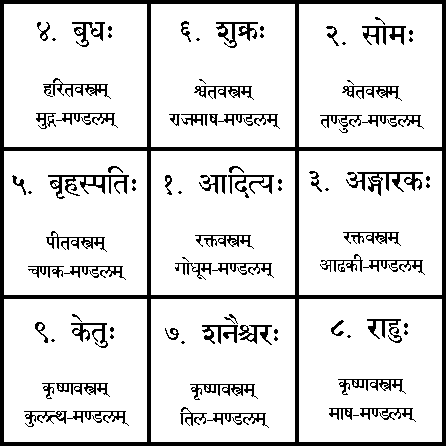
\includegraphics{purvanga/navagraha-diagram.pdf}

\twolineshloka
{जपाकुसुमसङ्काशं काश्यपेयं महद्युतिम्}
{तमोऽरिं सर्वपापघ्नं प्रणतोऽस्मि दिवाकरम्}

आ स॒त्येन॒ रज॑सा॒ वर्त॑मानो निवे॒शय॑न्न॒मृतं॒ मर्त्यं॑ च। हि॒र॒ण्यये॑न सवि॒ता रथे॒नाऽदे॒वो या॑ति॒
भुव॑ना वि॒पश्य\sn{}। अ॒ग्निं दू॒तं वृ॑णीमहे॒ होता॑रं वि॒श्ववे॑दसम्। अ॒स्य य॒ज्ञस्य॑ सु॒क्रतुम्॥
येषा॒मीशे॑ पशु॒पति॑ पशू॒नां चतु॑ष्पदामु॒त च॑ द्वि॒पदाम्। निष्क्री॑तो॒ऽयं य॒ज्ञियं॑ भा॒गमे॑तु
रा॒यस्पोषा॒ यज॑मानस्य सन्तु॥  अधिदेवता प्रत्यधिदेवता सहिताय आदित्याय॒ नम॥ 

अस्मिन् मण्डले अधिदेवता-प्रत्यधिदेवता-सहितं आदित्य-ग्रहं ध्यायामि। आवाहयामि।

\twolineshloka
{दधिशङ्खतुषाराभं क्षीरोदार्णवसम्भवम्}
{नमामि शशिनं सोमं शम्भोर्मुकुटभूषणम्}

आप्या॑यस्व॒ समे॑तु ते वि॒श्वत॑ सोम॒ वृष्णि॑यम्। भवा॒ वाज॑स्य सङ्ग॒थे॥ अ॒प्सु मे॒ सोमो॑
अब्रवीद॒न्तर्विश्वा॑नि भेष॒जा। अ॒ग्निं च॑ वि॒श्वश॑म्भुव॒माप॑श्च वि॒श्वभे॑षजीः। गौ॒री मि॑माय
सलि॒लानि॒ तक्ष॒ती। एक॑पदी द्वि॒पदी॒ सा चतु॑ष्पदी। अ॒ष्टाप॑दी॒ नव॑पदी बभू॒वुषी। स॒हस्राक्षरा पर॒मे
व्यो॑मन्।  अधिदेवता प्रत्यधिदेवता सहिताय सोमाय॒ नम॥ 

अस्मिन् मण्डले अधिदेवता-प्रत्यधिदेवता-सहितं सोम-ग्रहं ध्यायामि। आवाहयामि।


\twolineshloka
{धरणीगर्भसम्भूतं विद्युत्कान्तिसमप्रभम्}
{कुमारं शक्तिहस्तं च मङ्गलं प्रणमाम्यहम्}

अ॒ग्निर्मू॒र्द्धा दि॒वः क॒कुत्पति॑ पृथि॒व्या अ॒यम्। अ॒पा रेतासि जिन्वति। स्यो॒ना पृ॑थिवि॒
भवा॑ऽनृक्ष॒रा नि॒वेश॑नी। यच्छा॑न॒ शर्म॑ स॒प्रथा। क्षेत्र॑स्य॒ पति॑ना व॒य हि॒ते ने॑व जयामसि।
गामश्वं॑ पोषयि॒त्न्वा स नो॑ मृडाती॒दृशे॥  अधिदेवता प्रत्यधिदेवता सहिताय अङ्गारकाय॒ नम॥ 

अस्मिन् मण्डले अधिदेवता-प्रत्यधिदेवता-सहितं अङ्गारक-ग्रहं ध्यायामि। आवाहयामि।


\twolineshloka
{प्रियङ्गुकलिकाश्यामं रूपेणाप्रतिमं बुधम्}
{सौम्यं सौम्यगुणोपेतं तं बुधं प्रणमाम्यहम्}

उद्बु॑ध्यस्वाग्ने॒ प्रति॑जागृह्येनमिष्टापू॒र्ते ससृ॑जेथाम॒यं च॑। पुन॑ कृ॒ण्वस्त्वा॑ पि॒तरं॒
युवा॑नम॒न्वातासी॒त्वयि॒ तन्तु॑मे॒तम्॥ इ॒दं विष्णु॒र्विच॑क्रमे त्रे॒धा निद॑धे प॒दम्। समू॑ढमस्यपा
सु॒रे॥ विष्णो॑ र॒राट॑मसि॒ विष्णो पृ॒ष्ठम॑सि॒ विष्णो॒ श्नप्त्रेस्थो॒ विष्णो॒ स्यूर॑सि॒
विष्णोर्ध्रु॒वम॑सि वैष्ण॒वम॑सि॒ विष्ण॑वे त्वा।  अधिदेवता प्रत्यधिदेवता सहिताय बुधाय॒ नम॥ 

अस्मिन् मण्डले अधिदेवता-प्रत्यधिदेवता-सहितं बुध-ग्रहं ध्यायामि। आवाहयामि।


\twolineshloka
{देवानां च ऋषीणां च गुरुं काञ्चनसन्निभम्}
{बुद्धिभूतं त्रिलोकेशं तं नमामि बृहस्पतिम्}

बृह॑स्पते॒ अति॒यद॒र्यो अर्हाद्वि॒मद्वि॒भाति॒ क्रतु॑म॒ज्जने॑षु। यद्दी॒दय॒च्छव॑सर्त\-प्रजात॒
तद॒स्मासु॒ द्रवि॑णं धेहि चि॒त्रम्॥ इन्द्र॑मरुत्व इ॒ह पा॑हि॒ सोमं॒ यथा॑ शार्या॒ते अपि॑बः सु॒तस्य॑।
तव॒ प्रणी॑ती॒ तव॑ शूर॒शर्म॒न्नावि॑वासन्ति क॒वय॑ सुय॒ज्ञाः॥ ब्रह्म॑जज्ञा॒नं प्र॑थ॒मं
पु॒रस्ता॒द्विसी॑म॒तः सु॒रुचो॑ वे॒न आ॑वः। सबु॒ध्निया॑ उप॒मा अ॑स्य वि॒ष्ठाः स॒तश्च॒ योनि॒मस॑तश्च॒
विव॑॥ अधिदेवता प्रत्यधिदेवता सहिताय बृहस्पतये॒ नम॥ 

अस्मिन् मण्डले अधिदेवता-प्रत्यधिदेवता-सहितं बृहस्पति-ग्रहं ध्यायामि। आवाहयामि।

\twolineshloka
{हिमकुन्दमृणालाभं दैत्यानां परमं गुरुम्}
{सर्वशास्त्रप्रवक्तारं भार्गवं प्रणमाम्यहम्}

प्रव॑ शु॒क्राय॑ भा॒नवे॑ भरध्व ह॒व्यं म॒तिं चा॒ग्नये॒ सुपू॑तम्॥ यो दैव्या॑नि॒ मानु॑षा
ज॒नूष्य॒न्तर्विश्वा॑नि वि॒द्म ना॒ जिगा॑ति॥ इ॒न्द्रा॒णीमा॒सु नारि॑षु सु॒पत्नी॑म॒हम॑श्रवम्। न
ह्य॑स्या अप॒रञ्च॒न ज॒रसा॒ मर॑ते॒ पति॑॥ इन्द्रं॑ वो वि॒श्वत॒स्परि॒ हवा॑महे॒ जनेभ्यः। अ॒स्माक॑मस्तु॒
केव॑लः॥  अधिदेवता प्रत्यधिदेवता सहिताय शुक्राय॒ नम॥ 

अस्मिन् मण्डले अधिदेवता-प्रत्यधिदेवता-सहितं शुक्र-ग्रहं ध्यायामि। आवाहयामि।

\twolineshloka
{नीलाञ्जनसमाभासं रविपुत्रं यमाग्रजम्}
{छायामार्तण्डसम्भूतं तं नमामि शनैश्चरम्}

शं नो॑ दे॒वीर॒भिष्ट॑य॒ आपो॑ भवन्तु पी॒तये। शंयोर॒भिस्र॑वन्तु नः॥ प्रजा॑पते॒ न त्वदे॒तान्य॒न्यो
विश्वा॑ जा॒तानि॒ परि॒ता ब॑भूव। यत्का॑मास्ते जुहु॒मस्तन्नो॑ अस्तु व॒य स्या॑म॒ पत॑यो रयी॒णाम्। इ॒मं
य॑मप्रस्त॒रमाहि सीदाऽङ्गि॑रोभिः पि॒तृभि॑ संविदा॒नः। आत्वा॒ मन्त्रा कविश॒स्ता व॑हन्त्वे॒ना रा॑जन्
ह॒विषा॑ मादयस्व॥  अधिदेवता प्रत्यधिदेवता सहिताय शनैश्चराय॒ नम॥ 

अस्मिन् मण्डले अधिदेवता-प्रत्यधिदेवता-सहितं शनैश्चर-ग्रहं ध्यायामि। आवाहयामि।

\twolineshloka
{अर्धकायं महावीर्यं चन्द्रादित्यविमर्दनम्}
{सिंहिकागर्भसम्भूतं तं राहुं प्रणमाम्यहम्}

कया॑ नश्चि॒त्र आभु॑वदू॒ती स॒दावृ॑ध॒ सखा। कया॒ शचि॑ष्ठया वृ॒ता। आऽयङ्गौः
पृश्नि॑रक्रमी॒दस॑नन्मा॒तरं॒ पुन॑। पि॒तरं॑ च प्र॒यन्त्सुव॑। यत्ते॑ दे॒वी निर्ऋ॑तिराब॒बन्ध॒ दाम॑
ग्री॒वास्व॑विच॒र्त्यम्। इ॒दं  ते॒ तद्विष्या॒म्यायु॑षो॒ न मध्या॒दथा॑जी॒वः पि॒तुम॑द्धि॒ प्रमु॑क्तः॥ 
अधिदेवता प्रत्यधिदेवता सहिताय राहवे॒ नम॥ 

अस्मिन् मण्डले अधिदेवता-प्रत्यधिदेवता-सहितं राहु-ग्रहं ध्यायामि। आवाहयामि।

\twolineshloka
{पलाशपुष्पसङ्काशं तारकाग्रहमस्तकम्}
{रौद्रं रौद्रात्मकं घोरं तं केतुं प्रणमाम्यहम्}

के॒तुं कृ॒ण्वन्न॑के॒तवे॒ पेशो॑ मर्या अपे॒शसे। समु॒षद्भि॑रजायथाः॥ ब्र॒ह्मा दे॒वानां पद॒वीः
क॑वी॒नामृषि॒र्विप्रा॑णां महि॒षो मृ॒गाणाम्। श्ये॒नो गृध्रा॑णा॒ स्वधि॑ति॒र्वना॑ना॒ सोम॑
प॒वित्र॒मत्ये॑ति॒ रेभ\sn{}। (ऋक्) सचि॑त्र चि॒त्रं चि॒तयन् तम॒स्मे चित्र॑क्षत्र चि॒त्रत॑मं वयो॒धाम्।
च॒न्द्रं र॒यिं पु॑रु॒वीरं बृ॒हन्तं॒ चन्द्र॑च॒न्द्राभि॑र्गृण॒ते यु॑वस्व॥  अधिदेवता प्रत्यधिदेवता
सहिताय केतवे॒ नम॥ 

अस्मिन् मण्डले अधिदेवता-प्रत्यधिदेवता-सहितं केतु-ग्रहं ध्यायामि। आवाहयामि।

आदित्यादि नवग्रहदेवताभ्यो नमः आसनं समर्पयामि।
पाद्यं समर्पयामि। अर्घ्यं समर्पयामि। आचमनीयं समर्पयामि। 

शुद्धोदकस्नानं समर्पयामि। स्नानानन्तरम् आचमनीयं समर्पयामि।
वस्त्रार्थम् अक्षतान् समर्पयामि।\\
यज्ञोपवीताभरणार्थे अक्षतान् समर्पयामि।\\
दिव्यपरिमलगन्धान् धारयामि।\\
गन्धस्योपरि हरिद्राकुङ्कुमं समर्पयामि। अक्षतान् समर्पयामि। \\
पुष्पैः पूजयामि।

\begin{enumerate}%[label=\devanumber\value{enumi}]
\item ॐ आदित्याय नमः
\item ॐ अङ्गारकाय नम​:
\item ॐ शुक्राय नमः
\item ॐ सोमाय नम​:
\item ॐ बुधाय नम​:
\item ॐ बृहस्पतये नमः
\item ॐ शनैश्चराय नमः
\item ॐ राहवे नमः
\item ॐ केतवे नम​:
\end{enumerate}

नानाविध-परिमल-पत्र-पुष्पाणि समर्पयामि।

आदित्यादि नवग्रहदेवताभ्यो नमः धूपमाघ्रापयामि।\\
दीपं दर्शयामि।\\
नैवेद्यम्। \\
कर्पूरताम्बूलं समर्पयामि। कर्पूरनीराजनं दर्शयामि।\\
प्रार्थनाः समर्पयामि।
अनन्तकोटिप्रदक्षिणनमस्कारान् समर्पयामि।\\

आदित्यादि नवग्रहदेवताभ्यो नमः (अक्षतान् समर्पयित्वा) यथास्थानं प्रतिष्ठापयामि। शोभनार्थे क्षेमाय पुनरागमनाय च।


% !TeX program = XeLaTeX
% !TeX root = ..\pujavidhanam.tex

\sect{लोकपालपूजा}

प्राणान् आयम्य। ममोपात्तसमस्तदुरितक्षयद्वारा श्रीपरमेश्वरप्रीत्यर्थम् अद्य-पूर्वोक्त एवं गुण-विशेषेण विशिष्टायाम् अस्यां
अमावास्यायां शुभतिथौ श्रीमहालक्ष्मी-पूजाङ्गभूतां ब्रह्म-विष्णु-त्र्यम्बक-क्षेत्रपाल-पूजां करिष्ये।

अस्मिन् कूर्चे ब्रह्मादीन् ध्यायामि। ब्रह्मन् सरस्वत्या सह इह आगच्छ आगच्छ। सरस्वती-सहित-ब्रह्माणम् आवाहयामि। आसनं समर्पयामि।

लक्ष्मी-विष्णुभ्यां नमः।\\
ध्यायामि। आवाहयामि। आसनं समर्पयामि।

दुर्गा-त्र्यम्बकाभ्यां नमः।\\
ध्यायामि। आवाहयामि। आसनं समर्पयामि।

क्षेत्रपाल-भूमिभ्यां नमः।\\
ध्यायामि। आवाहयामि। आसनं समर्पयामि।

ब्रह्मादिभ्यो नमः पाद्यं समर्पयामि। अर्घ्यं समर्पयामि।
आचमनीयं समर्पयामि। शुद्धोदकस्नानं समर्पयामि। स्नानानन्तरम् आचमनीयं समर्पयामि।
वस्त्रार्थम् अक्षतान् समर्पयामि।
यज्ञोपवीताभरणार्थे अक्षतान् समर्पयामि।
दिव्यपरिमलगन्धान् धारयामि।
गन्धस्योपरि हरिद्राकुङ्कुमं समर्पयामि। अक्षतान् समर्पयामि। \\
पुष्पैः पूजयामि।\\

नैवेद्यम्। \\
कर्पूरताम्बूलं समर्पयामि। कर्पूरनीराजनं दर्शयामि।\\
प्रार्थनाः समर्पयामि।
अनन्तकोटिप्रदक्षिणनमस्कारान् समर्पयामि।\\

ब्रह्मादिभ्यो नमः (अक्षतान् समर्पयित्वा) यथास्थानं प्रतिष्ठापयामि। शोभनार्थे क्षेमाय पुनरागमनाय च।

\dnsub{प्रार्थना}

\twolineshloka*
{विघ्नराजं नमस्कृत्य नमस्कृत्य विधिं परम्}
{विष्णुं रुद्रं श्रियं दुर्गां वन्दे भक्त्या सरस्वतीम्}

\twolineshloka*
{क्षेत्राधिपं नमस्कृत्य दिवानाथं निशाकरम्}
{धरणीगर्भसम्भूतं शशिपुत्रं बृहस्पतिम्}

\twolineshloka*
{दैत्याचार्यं नमस्कृत्य सूर्यपुत्रं महाग्रहम्}
{राहुकेतू नमस्कृत्य यज्ञारम्भे विशेषतः}

\twolineshloka*
{शक्राद्या देवताः सर्वाः मुनींश्च प्रणमाम्यहम्}
{गर्गं मुनिं नमस्कृत्य नारदं मुनिसत्तमम्}

\twolineshloka*
{वसिष्ठं मुनिशार्दूलं विश्वामित्रं भृगोः सुतम्}
{व्यासं मुनिं नमस्कृत्य आचार्यांश्च तपोधनान्}

\twolineshloka*
{सर्वान् तान् प्रणमाम्येवं यज्ञरक्षाकरान् सदा}
{शङ्खचक्रगदाशार्ङ्ग-पद्मपाणिर्जनार्दनः}
\onelineshloka*
{सर्वासु दिक्षु रक्षेन्मां यावत् पूजावसानकम्}


\sect{षोडशोपचारपूजा}
\begin{center}
\fourlineindentedshloka*
{अरुणकमलसंस्था तद्रजःपुञ्जवर्णा}
{करकमलधृतेष्टाऽभीतियुग्माम्बुजा च}
{मणिमकुटविचित्रालङ्कृता कल्पजातैः}
{भवतु भुवनमाता सन्ततं श्रीः श्रियै नः}

अस्मिन् बिम्बे श्रीमहालक्ष्मीं ध्यायामि।

\twolineshloka*
{आवाहये महालक्ष्मि चैतन्यस्तन्यदायिनि}
{विष्णुपत्नि जगन्मातः पूजां गृह्णीष्व ते नमः}
श्रीमहालक्ष्मीम् आवाहयामि।

\twolineshloka*
{तप्तकाञ्चनवर्णाभं मुक्तामणिविराजितम्}
{अमलं कमलं दिव्यम् आसनं प्रतिगृह्यताम्}
 आसनं समर्पयामि।\medskip


\twolineshloka*
{गङ्गातीर्थ-समुद्भूतं गन्ध-पुष्पादिभिर्युतम्}
{पाद्यं ददाम्यहं देवि गृहाणाऽऽशु नमोऽस्तु ते}
 पाद्यं समर्पयामि।\medskip

\twolineshloka*
{एलागन्धसमायुक्तं स्वर्णपात्रे प्रपूरितम्}
{अर्घ्यं गृहाण मद्दत्तं प्रसीद त्वं महेश्वरि}
 अर्घ्यं समर्पयामि।\medskip


\twolineshloka*
{सर्वलोकस्य या शक्तिः ब्रह्मरुद्रादिभिः स्तुता}
{ददाम्याचमनं तस्यै महालक्ष्म्यै मनोहरम्}
 आचमनीयं समर्पयामि।\medskip

घृतेन स्नपयामि। पुनः शुद्धोदकं समर्पयामि।\\
पयसा स्नपयामि। पुनः शुद्धोदकं समर्पयामि।\\
दध्ना स्नपयामि। पुनः शुद्धोदकं समर्पयामि।\\
मधुना स्नपयामि। पुनः शुद्धोदकं समर्पयामि।\\
पञ्चामृतेन स्नपयामि। पुनः शुद्धोदकं समर्पयामि।

(कलशजलेन श्री-सूक्तं जप्य) शुद्धोदकस्नानं समर्पयामि।
स्नानानन्तरम् आचमनीयं समर्पयामि।\medskip

\twolineshloka*
{दिव्याम्बरयुगं सूक्ष्मं कञ्चुकं च मनोहरम्}
{महालक्ष्मि महादेवि गृहाणेदं मयाऽर्पितम्}
 वस्त्रं समर्पयामि।\medskip

\twolineshloka*
{माङ्गल्यमणिसंयुक्तं मुक्ताविद्रुमसंयुतम्}
{दत्तं मङ्गलसूत्रं च गृहाण हरिवल्लभे}
कण्ठसूत्रं समर्पयामि।\medskip


\twolineshloka*
{रत्नकङ्कणवैडूर्य-मुक्ताहारादिकानि च}
{सुप्रसन्नेन मनसा दत्तानि त्वं गृहाण मे}
आभरणानि समर्पयामि।\medskip

\twolineshloka*
{सिन्दूरारुणवर्णा च सिन्दूरतिलकप्रिया}
{अतो दत्तं मया देवि सिन्दूरं प्रतिगृह्यताम्}
 तिलकं समर्पयामि। \medskip

\twolineshloka*
{मन्दार-पारिजाताद्याः पाटली केतकी तथा}
{माकन्दं कुरवं चैव गृहाणाऽऽशु नमोऽस्तु ते}
  पुष्पमालां धारयामि। 
\end{center}
\dnsub{अङ्गपूजा}
\begin{longtable}{ll@{— }l}
१.& ॐ चपलायै नमः & पादौ पूजयामि \\
२.& चञ्चलायै नमः & जानुनी पूजयामि\\
३.& कमलायै नमः & कटिं पूजयामि  \\
४.& कात्यायन्यै नमः & नाभिं पूजयामि\\
५.& जगन्मात्रे नमः & जठरं पूजयामि   \\
६.& विश्ववल्लभायै नमः & वक्षःस्थलं पूजयामि \\
७.& कमलवासिन्यै नमः & हस्तौ पूजयामि        \\
८.& पद्माननायै नमः & मुखं पूजयामि\\
९.& कमलपत्राक्ष्यै नमः & नेत्रत्रयं पूजयामि    \\
१०.& श्रियै नमः & शिरः पुजयामि\\
११.& महालक्ष्म्यै नमः & सर्वाणि अङ्गानि पूजयामि   \\
\end{longtable}

\dnsub{अष्टलक्ष्मी-अर्चना}
(प्राच्याम् आरभ्य अष्टदिक्षु प्रदक्षिणेन)

\begin{multicols}{2}
\begin{enumerate}
\item ॐ आद्यलक्ष्म्यै नमः
\item ॐ विद्यालक्ष्म्यै नमः
\item ॐ सौभाग्यलक्ष्म्यै नमः
\item ॐ अमृतलक्ष्म्यै नमः
\item ॐ कामलक्ष्म्यै नमः 
\item ॐ सत्यलक्ष्म्यै नमः
\item ॐ भोगलक्ष्म्यै नमः
\item ॐ योगलक्ष्म्यै नमः
\end{enumerate}
\end{multicols}

आद्यादिलक्ष्मीनां षोडशोपचारपूजार्थे पुष्पाणि समर्पयामि।

\dnsub{लक्ष्म्यष्टोत्तरशतनामावलिः}
\begin{multicols}{2}
\begin{flushleft}
ॐ प्रकृत्यै~नमः\\
ॐ विकृत्यै~नमः\\
ॐ विद्यायै~नमः\\
ॐ सर्वभूतहितप्रदायै~नमः\\
ॐ श्रद्धायै~नमः\\
ॐ विभूत्यै~नमः\\
ॐ सुरभ्यै~नमः\\
ॐ परमात्मिकायै~नमः\\
ॐ वाचे~नमः\\
ॐ पद्मालयायै~नमः\hfill\devanumber{10}\\
ॐ पद्मायै~नमः\\
ॐ शुचये~नमः\\
ॐ स्वाहायै~नमः\\
ॐ स्वधायै~नमः\\
ॐ सुधायै~नमः\\
ॐ धन्यायै~नमः\\
ॐ हिरण्मय्यै~नमः\\
ॐ लक्ष्म्यै~नमः\\
ॐ नित्यपुष्टायै~नमः\\
ॐ विभावर्यै~नमः\hfill\devanumber{20}\\
ॐ अदित्यै~नमः\\
ॐ दित्यै~नमः\\
ॐ दीप्तायै~नमः\\
ॐ वसुधायै~नमः\\
ॐ वसुधारिण्यै~नमः\\
ॐ कमलायै~नमः\\
ॐ कान्तायै~नमः\\
ॐ कामायै~नमः\\
ॐ क्षीरोदसम्भवायै~नमः\\
ॐ अनुग्रहपदायै~नमः\hfill\devanumber{30}\\
ॐ बुद्धये~नमः\\
ॐ अनघायै~नमः\\
ॐ हरिवल्लभायै~नमः\\
ॐ अशोकाममृतायै~नमः\\
ॐ दीप्तायै~नमः\\
ॐ लोकशोकविनाशिन्यै~नमः\\
ॐ धर्मनिलयायै~नमः\\
ॐ करुणायै~नमः\\
ॐ लोकमात्रे~नमः\\
ॐ पद्मप्रियायै~नमः\hfill\devanumber{40}\\
ॐ पद्महस्तायै~नमः\\
ॐ पद्माक्ष्यै~नमः\\
ॐ पद्मसुन्दर्यै~नमः\\
ॐ पद्मोद्भवायै~नमः\\
ॐ पद्ममुख्यै~नमः\\
ॐ पद्मनाभप्रियायै~नमः\\
ॐ रमायै~नमः\\
ॐ पद्ममालाधरायै~नमः\\
ॐ देव्यै~नमः\\
ॐ पद्मिन्यै~नमः\hfill\devanumber{50}\\
ॐ पद्मगन्धिन्यै~नमः\\
ॐ पुण्यगन्धायै~नमः\\
ॐ सुप्रसन्नायै~नमः\\
ॐ प्रसादाभिमुख्यै~नमः\\
ॐ प्रभायै~नमः\\
ॐ चन्द्रवदनायै~नमः\\
ॐ चन्द्रायै~नमः\\
ॐ चन्द्रसहोदर्यै~नमः\\
ॐ चतुर्भुजायै~नमः\\
ॐ चन्द्ररूपायै~नमः\hfill\devanumber{60}\\
ॐ इन्दिरायै~नमः\\
ॐ इन्दुशीतलायै~नमः\\
ॐ आह्लादजनन्यै~नमः\\
ॐ पुष्ट्यै~नमः\\
ॐ शिवायै~नमः\\
ॐ शिवकर्यै~नमः\\
ॐ सत्यै~नमः\\
ॐ विमलायै~नमः\\
ॐ विश्वजनन्यै~नमः\\
ॐ तुष्ट्यै~नमः\hfill\devanumber{70}\\
ॐ दारिद्र्यनाशिन्यै~नमः\\
ॐ प्रीतिपुष्करिण्यै~नमः\\
ॐ शान्तायै~नमः\\
ॐ शुक्लमाल्याम्बरायै~नमः\\
ॐ श्रियै~नमः\\
ॐ भास्कर्यै~नमः\\
ॐ बिल्वनिलयायै~नमः\\
ॐ वरारोहायै~नमः\\
ॐ यशस्विन्यै~नमः\\
ॐ वसुन्धरायै~नमः\hfill\devanumber{80}\\
ॐ उदाराङ्गायै~नमः\\
ॐ हरिण्यै~नमः\\
ॐ हेममालिन्यै~नमः\\
ॐ धनधान्यकर्यै~नमः\\
ॐ सिद्ध्यै~नमः\\
ॐ स्त्रैणसौम्यायै~नमः\\
ॐ शुभप्रदायै~नमः\\
ॐ नृपवेश्मगतानन्दायै~नमः\\
ॐ वरलक्ष्म्यै~नमः\\
ॐ वसुप्रदायै~नमः\hfill\devanumber{90}\\
ॐ शुभायै~नमः\\
ॐ हिरण्यप्राकारायै~नमः\\
ॐ समुद्रतनयायै~नमः\\
ॐ जयायै~नमः\\
ॐ मङ्गलायै~नमः\\
ॐ देव्यै~नमः\\
ॐ~विष्णुवक्षःस्थल\-स्थितायै~नमः\\
ॐ विष्णुपत्न्यै~नमः\\
ॐ प्रसन्नाक्ष्यै~नमः\\
ॐ नारायणसमाश्रितायै~नमः\hfill\devanumber{100}\\
ॐ दारिद्र्यध्वंसिन्यै~नमः\\
ॐ देव्यै~नमः\\
ॐ सर्वोपद्रवहारिण्यै~नमः\\
ॐ नवदुर्गायै~नमः\\
ॐ महाकाल्यै~नमः\\
ॐ~ब्रह्मविष्णुशिवात्मिकायै नमः\\
ॐ त्रिकालज्ञानसम्पन्नायै~नमः\\
ॐ भुवनेश्वर्यै~नमः\\
\end{flushleft}
\end{multicols}

\sect{उत्तराङ्गपूजा}

\begin{center}

\twolineshloka*
{वनस्पति-रसोत्पन्नो गन्धाढ्यो गन्ध उत्तमः}
{आघ्रेयः सर्वदेवानां धूपोऽयं प्रतिगृह्यताम्}
श्री महालक्ष्म्यै नमः धूपमाघ्रापयामि।\\
 
\twolineshloka*
{कार्पासवर्तिसंयुक्तं घृतयुक्तं मनोहरम्}
{तमोनाशकरं दीपं गृहाण परमेश्वर}
श्री महालक्ष्म्यै नमः अलङ्कारदीपं सन्दर्शयामि।\\

\twolineshloka*
{नैवेद्यं गृह्यतां लक्ष्मि भक्ष्य-भोज्य-समन्वितम्}
{षड्रसैर्रचितं दिव्यं लक्ष्मीदेवि नमोऽस्तु ते}
नैवेद्यम्\\
- श्री महालक्ष्म्यै नमः (	) निवेदयामि, \\
अमृतापिधानमसि। निवेदनानन्तरम् आचमनीयं समर्पयामि।\\

पूगीफलसमायुक्तं नागवल्लीदलैर्युतम्।\\
कर्पूरचूर्णसंयुक्तं ताम्बूलं प्रतिगृह्यताम्॥\\
श्री महालक्ष्म्यै नमः कर्पूरताम्बूलं समर्पयामि।\\

श्री महालक्ष्म्यै नमः समस्त अपराध क्षमापनार्थं कर्पूरनीराजनं दर्शयामि।\\
कर्पूरनीरजनानन्तरम् आचमनीयं समर्पयामि।\\

 यो॑ऽपां पुष्पं॒ वेद॑। पुष्प॑वान् प्र॒जावान् पशु॒मान् भ॑वति।\\
च॒न्द्रमा॒ वा अ॒पां पुष्पम्। पुष्प॑वान् प्र॒जावान् पशु॒मान् भ॑वति।\\
य ए॒वं वेद॑। यो॑ऽपामा॒यत॑नं॒ वेद॑। आ॒यत॑नवान् भवति।\\

ओं तद्ब्र॒ह्म। ओं तद्वा॒युः। ओं तदा॒त्मा। ओं᳚ तथ्स॒त्यम्‌।\\
ओं᳚ तथ्सर्वम्᳚‌। ओं तत्पुरो॒र्नमः॥\\

अन्तश्चरति॑ भूते॒षु॒ गुहायां वि॑श्वमू॒र्तिषु। \\
त्वं यज्ञस्त्वं वषट्कारस्त्वमिन्द्रस्त्व रुद्रस्त्वं विष्णुस्त्वं ब्रह्म त्वं॑ प्रजा॒पतिः। \\
त्वं त॑दाप॒ आपो॒ ज्योती॒ रसो॒ऽमृतं॒ ब्रह्म॒ भूर्भुव॒स्सुव॒रोम्‌॥\\

श्री महालक्ष्म्यै नमः वेदोक्तमन्त्रपुष्पाञ्जलिं समर्पयामि।\\

स्वर्णपुष्पं समर्पयामि\\
 
अनन्तकोटिप्रदक्षिणनमस्कारान् समर्पयामि\\

छत्त्रचामरादिसमस्तोपचारान् समर्पयामि\\

हिरण्यगर्भगर्भस्थं हेमबीजं विभावसोः।\\
अनन्तपुण्यफलदम् अतः शान्तिं प्रयच्छ मे॥\\

आश्वयुज-अमावास्या-पुण्यकालेऽस्मिन् मया क्रियमाण श्री\-महा\-लक्ष्मी-पूजायां
यद्देयमुपायन\-दानं तत्प्रति\-निधित्वेन हिरण्यं श्री महा\-लक्ष्मी\-प्रीतिं
कामयमानः मनसोद्दिष्टाय ब्राह्मणाय सम्प्रददे नमः न मम। 
अनया पूजया श्री महालक्ष्मीः प्रीयताम्। 
\end{center}

\sect{ईशानादि पूजा}

\sect{कुबेर पूजा}



\dnsub{कुबेराष्टोत्तरशतनामावलिः}

\fourlineindentedshloka*
{मनुजबाह्यविमानवरस्तुतम्}
{गरुडरत्ननिभं निधिनायकम्}
{शिवसखं मुकुटादिविभूषितम्}
{वररुचिं तमहमुपास्महे सदा}

\twolineshloka*
{अगस्त्य देवदेवेश मर्त्यलोकहितेच्छया}
{पूजयामि विधानेन प्रसन्नसुमुखो भव}
\begin{multicols}{2}
\begin{flushleft}
ॐ कुबेराय नमः\\
ॐ धनदाय नमः\\
ॐ श्रीमते नमः\\
ॐ यक्षेशाय नमः\\
ॐ गुह्यकेश्वराय नमः\\
ॐ निधीशाय नमः\\
ॐ शङ्करसखाय नमः\\
ॐ महालक्ष्मीनिवासभुवे नमः\\
ॐ महापद्मनिधीशाय नमः\\
ॐ पूर्णाय नमः\hfill\devanumber{10}\\ %१०
ॐ पद्मनिधीश्वराय नमः\\
ॐ शङ्खाख्यनिधिनाथाय नमः\\
ॐ मकराख्यनिधिप्रियाय नमः\\
ॐ सुकच्छपाख्यनिधीशाय नमः\\
ॐ मुकुन्दनिधिनायकाय नमः\\
ॐ कुन्दाख्यनिधिनाथाय नमः\\
ॐ नीलनित्याधिपाय नमः\\
ॐ महते नमः\\
ॐ वरनिधिदीपाय नमः\\
ॐ पूज्याय नमः\hfill\devanumber{20}\\ %२०
ॐ लक्ष्मीसाम्राज्यदायकाय नमः\\
ॐ इलपिलापत्याय नमः\\
ॐ कोशाधीशाय नमः\\
ॐ कुलोचिताय नमः\\
ॐ अश्वारूढाय नमः\\
ॐ विश्ववन्द्याय नमः\\
ॐ विशेषज्ञाय नमः\\
ॐ विशारदाय नमः\\
ॐ नलकूबरनाथाय नमः\\
ॐ मणिग्रीवपित्रे नमः\hfill\devanumber{30}\\ %३०
ॐ गूढमन्त्राय नमः\\
ॐ वैश्रवणाय नमः\\
ॐ चित्रलेखामनःप्रियाय नमः\\
ॐ एकपिनाकाय नमः\\
ॐ अलकाधीशाय नमः\\
ॐ पौलस्त्याय नमः\\
ॐ नरवाहनाय नमः\\
ॐ कैलासशैलनिलयाय नमः\\
ॐ राज्यदाय नमः\\
ॐ रावणाग्रजाय नमः\hfill\devanumber{40}\\ %४०
ॐ चित्रचैत्ररथाय नमः\\
ॐ उद्यानविहाराय नमः\\
ॐ विहारसुकुतूहलाय नमः\\
ॐ महोत्सहाय नमः\\
ॐ महाप्राज्ञाय नमः\\
ॐ सदापुष्पकवाहनाय नमः\\
ॐ सार्वभौमाय नमः\\
ॐ अङ्गनाथाय नमः\\
ॐ सोमाय नमः\\
ॐ सौम्यादिकेश्वराय नमः\hfill\devanumber{50}\\ %५०
ॐ पुण्यात्मने नमः\\
ॐ पुरुहुतश्रियै नमः\\
ॐ सर्वपुण्यजनेश्वराय नमः\\
ॐ नित्यकीर्तये नमः\\
ॐ निधिवेत्रे नमः\\
ॐ लङ्काप्राक्तननायकाय नमः\\
ॐ यक्षिणीवृताय नमः\\
ॐ यक्षाय नमः\\
ॐ परमशान्तात्मने नमः\\
ॐ यक्षराजे नमः\hfill\devanumber{60}\\ %६०
ॐ यक्षिणीहृदयाय नमः\\ 
ॐ किन्नरेश्वराय नमः\\
ॐ किम्पुरुषनाथाय नमः\\
ॐ खड्गायुधाय नमः\\
ॐ वशिने नमः\\
ॐ ईशानदक्षपार्श्वस्थाय नमः\\
ॐ वायुवामसमाश्रयाय नमः\\
ॐ धर्ममार्गनिरताय नमः\\
ॐ धर्मसम्मुखसंस्थिताय नमः\\
ॐ नित्येश्वराय नमः\hfill\devanumber{70}\\ %७०
ॐ धनाध्यक्षाय नमः\\
ॐ अष्टलक्ष्म्याश्रितालयाय नमः\\
ॐ मनुष्यधर्मिणे नमः\\
ॐ सुकृतिने नमः\\
ॐ कोषलक्ष्मीसमाश्रिताय नमः\\
ॐ धनलक्ष्मीनित्यवासाय नमः\\
ॐ धान्यलक्ष्मीनिवासभुवे नमः\\
ॐ अष्टलक्ष्मीसदावासाय नमः\\
ॐ गजलक्ष्मीस्थिरालयाय नमः\\
ॐ राज्यलक्ष्मीजन्मगेहाय नमः\hfill\devanumber{80}\\ %८०
ॐ धैर्यलक्ष्मीकृपाश्रयाय नमः\\
ॐ अखण्डैश्वर्यसंयुक्ताय नमः\\
ॐ नित्यानन्दाय नमः\\
ॐ सुखाश्रयाय नमः\\
ॐ नित्यतृप्ताय नमः\\
ॐ निराशाय नमः\\
ॐ निरुपद्रवाय नमः\\
ॐ नित्यकामाय नमः\\
ॐ निराकाङ्क्षाय नमः\\
ॐ निरूपाधिकवासभुवे नमः\hfill\devanumber{90}\\ %९०
ॐ शान्ताय नमः\\
ॐ सर्वगुणोपेताय नमः\\
ॐ सर्वज्ञाय नमः\\
ॐ सर्वसम्मताय नमः\\
ॐ सर्वाणिकरुणापात्राय नमः\\
ॐ सदानन्दकृपालयाय नमः\\
ॐ गन्धर्वकुलसंसेव्याय नमः\\
ॐ सौगन्धिककुसुमप्रियाय नमः\\
ॐ स्वर्णनगरीवासाय नमः\\
ॐ निधिपीठसमाश्रयाय नमः\hfill\devanumber{100}\\ %१००
ॐ महामेरूत्तरस्थाय नमः\\
ॐ महर्षिगणसंस्तुताय नमः\\
ॐ तुष्टाय नमः\\
ॐ शूर्पणखाज्येष्ठाय नमः\\
ॐ शिवपूजारताय नमः\\
ॐ अनघाय नमः\\
ॐ राजयोगसमायुक्ताय नमः\\
ॐ राजशेखरपूज्याय नमः\\
ॐ राजराजाय नमः\\ %१०९
\end{flushleft}
\end{multicols}


\sect{प्रार्थना}
\sect{अपराध-क्षमापनम्}
% \input{pujas/govardhana-puja.tex}
% % !TeX program = XeLaTeX
% !TeX root = ../pujavidhanam.tex

\setlength{\parindent}{0pt}
\chapt{श्री-स्कन्द-षष्ठी-पूजा}

\sect{पूर्वाङ्गविघ्नेश्वरपूजा}

(आचम्य)
\twolineshloka*
{शुक्लाम्बरधरं विष्णुं शशिवर्णं चतुर्भुजम्}
{प्रसन्नवदनं ध्यायेत् सर्वविघ्नोपशान्तये}
 
प्राणान्  आयम्य।  ॐ भूः + भूर्भुवः॒ सुव॒रोम्।
 
(अप उपस्पृश्य, पुष्पाक्षतान् गृहीत्वा)\\
ममोपात्तसमस्त दुरितक्षयद्वारा \\
श्रीपरमेश्वरप्रीत्यर्थं करिष्यमाणस्य कर्मणः\\
 निर्विघ्नेन परिसमाप्त्यर्थम् आदौ विघ्नेश्वरपूजां करिष्ये।

\twolineshloka*
{ॐ ग॒णानां᳚ त्वा ग॒णप॑तिꣳ हवामहे क॒विं क॑वी॒नामु॑प॒मश्र॑वस्तमम्}
{ज्ये॒ष्ठ॒राजं॒ ब्रह्म॑णां ब्रह्मणस्पत॒ आ नः॑ शृ॒ण्वन्नू॒तिभिः॑ सीद॒ साद॑नम्}
अस्मिन् हरिद्राबिम्बे महागणपतिं ध्यायामि, आवाहयामि।\\


ॐ महागणपतये नमः  आसनं समर्पयामि।\\
पादयोः पाद्यं समर्पयामि। हस्तयोरर्घ्यं समर्पयामि।\\
आचमनीयं समर्पयामि।\\
ॐ भूर्भुवस्सुवः। शुद्धोदकस्नानं समर्पयामि।\\
स्नानानन्तरमाचमनीयं समर्पयामि।\\
वस्त्रार्थमक्षतान् समर्पयामि।\\
यज्ञोपवीताभरणार्थे अक्षतान् समर्पयामि।\\
दिव्यपरिमलगन्धान् धारयामि।\\
गन्धस्योपरि हरिद्राकुङ्कुमं समर्पयामि। अक्षतान् समर्पयामि। \\
पुष्पमालिकां समर्पयामि। पुष्पैः पूजयामि।

\dnsub{अर्चना}
% \setenumerate{label=\devanumber.}
% \renewcommand{\labelenumi}{\devanumber\theenumi.}
\begin{enumerate}%[label=\devanumber\value{enumi}]
\begin{minipage}{0.475\linewidth}   
\item ॐ सुमुखाय नमः
\item ॐ एकदन्ताय नमः
\item ॐ कपिलाय नमः
\item ॐ गजकर्णकाय नमः
\item ॐ लम्बोदराय नमः
\item ॐ विकटाय नमः
\item ॐ विघ्नराजाय नमः
\item ॐ विनायकाय नमः
\item ॐ धूमकेतवे नमः
  \end{minipage}
  \begin{minipage}{0.525\linewidth}
\item ॐ गणाध्यक्षाय नमः
\item ॐ फालचन्द्राय नमः
\item ॐ गजाननाय नमः
\item ॐ वक्रतुण्डाय नमः
\item ॐ शूर्पकर्णाय नमः
\item ॐ हेरम्बाय नमः
\item ॐ स्कन्दपूर्वजाय नमः
\item ॐ सिद्धिविनायकाय नमः
\item ॐ विघ्नेश्वराय नमः
  \end{minipage}
\end{enumerate}
नानाविधपरिमलपत्रपुष्पाणि समर्पयामि॥\\
धूपमाघ्रापयामि।\\
अलङ्कारदीपं सन्दर्शयामि।\\
नैवेद्यम्।\\
ताम्बूलं समर्पयामि।\\
कर्पूरनीराजनं समर्पयामि।\\
कर्पूरनीराजनानन्तरमाचमनीयं समर्पयामि।\\
{वक्रतुण्डमहाकाय कोटिसूर्यसमप्रभ।}\\
{अविघ्नं कुरु मे देव सर्वकार्येषु सर्वदा॥}\\
प्रार्थनाः समर्पयामि।

अनन्तकोटिप्रदक्षिणनमस्कारान् समर्पयामि।\\
छत्त्रचामरादिसमस्तोपचारान् समर्पयामि।\\


\sect{प्रधान-पूजा — स्कन्द-पूजा}

\twolineshloka*
{शुक्लाम्बरधरं विष्णुं शशिवर्णं चतुर्भुजम्}
{प्रसन्नवदनं ध्यायेत् सर्वविघ्नोपशान्तये}

प्राणान् आयम्य। ॐ भूः + भूर्भुवः॒ सुव॒रोम्।


\dnsub{सङ्कल्पः}

ममोपात्त-समस्त-दुरित-क्षयद्वारा श्री-परमेश्वर-प्रीत्यर्थं शुभे शोभने मुहूत्ते अद्य ब्रह्मणः
द्वितीयपरार्द्धे श्वेतवराहकल्पे वैवस्वतमन्वन्तरे अष्टाविंशतितमे कलियुगे प्रथमे पादे
जम्बूद्वीपे भारतवर्षे भरतखण्डे मेरोः दक्षिणे पार्श्वे शकाब्दे अस्मिन् वर्तमाने व्यावहारिकाणां प्रभवादीनां षष्ट्याः संवत्सराणां मध्ये \mbox{(~~~)}\see{app:samvatsara_names} नाम संवत्सरे दक्षिणायने 
शरद्-ऋतौ  तुला/वृश्चिक-मासे कार्तिक-शुक्लपक्षे षष्ठ्यां शुभतिथौ
(इन्दु / भौम / बुध / गुरु / भृगु / स्थिर / भानु) वासरयुक्तायाम्
\mbox{(~~~)}\see{app:nakshatra_names} नक्षत्र \mbox{(~~~)}\see{app:yoga_names} नाम  योग  (कौलव/तैतिल) करण युक्तायां च एवं गुण विशेषण विशिष्टायाम् अस्यां षष्ठ्यां शुभतिथौ 

श्री-वल्ली-देवसेना-समेत-सुब्रह्मण्य-प्रीत्यर्थं प्रसाद-सिद्ध्यर्थम्
अस्माकं सहकुटुम्बानां क्षेमस्थैर्य-धैर्य-वीर्य-विजय-आयुरारोग्य-ऐश्वर्याणाम् अभिवृद्ध्यर्थं
धर्मार्थ\-काम\-मोक्ष\-चतुर्विध\-फल\-पुरुषार्थ\-सिद्ध्यर्थं पुत्र\-पौत्रा\-भि\-वृद्ध्यर्थम् इष्ट\-काम्यार्थ\-सिद्ध्यर्थं
मम इहजन्मनि पूर्वजन्मनि जन्मान्तरे च सम्पादितानां ज्ञानाज्ञानकृतमहा\-पातकचतुष्टय-व्यतिरिक्तानां रहस्यकृतानां प्रकाशकृतानां सर्वेषां पापानां सद्य अपनोदनद्वारा 
सकल-पाप\-क्षयार्थं गो-भू-धन-धान्य-पुत्र-पौत्रादि अनविच्छिन्न-सन्तति स्थिर-लक्ष्मी-कीर्ति-लाभ शत्रु-पराजयादि सदभीष्ट-सिद्ध्यर्थं दिव्यज्ञान-सिद्ध्यर्थं

यावच्छक्ति-ध्यानावाहनादि षोडशोपचारैः कल्पोक्त-प्रकारेण श्री-वल्ली-देवसेना-समेत-सुब्रह्मण्य-पूजाराधनं करिष्ये। तदङ्गं कलश\-पूजां च करिष्ये।


श्रीविघ्नेश्वराय नमः, यथास्थानं प्रतिष्ठापयामि।\\
(गणपति-प्रसादं शिरसा गृहीत्वा)


\dnsub{घण्टापूजा}
\twolineshloka*
{आगमार्थं तु देवानां गमनार्थं तु रक्षसाम्}
{कुरु घण्टारवं तत्र देवताऽऽह्वानलाञ्चनम्}


\dnsub{कलशपूजा}
(कलशं गन्धपुष्पाक्षतैः अभ्यर्च्य)

गङ्गायै नमः। यमुनायै नमः। गोदावर्यै नमः। सरस्वत्यै नमः। नर्मदायै नमः। सिन्धवे नमः। कावेर्यै नमः।\\
सप्तकोटिमहातीर्थान्यावाहयामि। \\

(अथ कलशं स्पृष्ट्वा जपं कुर्यात्।)

\twolineshloka*
{कलशस्य मुखे विष्णुः कण्ठे रुद्रः समाश्रितः}
{मूले तत्र स्थितो ब्रह्मा मध्ये मातृगणाः स्मृताः}

\threelineshloka*
{कुक्षौ तु सागराः सर्वे सप्तद्वीपा वसुन्धरा}
{ऋग्वेदोऽथ यजुर्वेदः सामवेदोऽप्यथर्वणः}
{अङ्गैश्च सहिताः सर्वे कलशाम्बुसमाश्रिताः}

\twolineshloka*
{गङ्गे च यमुने चैव गोदावरि सरस्वति}
{नर्मदे सिन्धुकावेरि जलेऽस्मिन् सन्निधिं कुरु}

\twolineshloka*
{सर्वे समुद्राः सरितः तीर्थानि च ह्रदा नदाः}
{आयान्तु विष्णुपूजार्थं दुरितक्षयकारकाः}

% \centerline{ॐ भूर्भुवः॒ सुवो॒ भूर्भुवः॒ सुवो॒ भूर्भुवः॒ सुवः॑।}

(इति कलशजलेन सर्वोपकरणानि आत्मानं च प्रोक्ष्य।)

\dnsub{आत्मपूजा}
आत्मने नमः, दिव्यगन्धान् धारयामि। 


\dnsub{मण्टप-पूजा}

ॐ ह्रीं श्रीं मण्डूकादि-परतत्त्वात्म-पर्यन्त-पीठ-शक्ति-देवताभ्यो नमः।\\
ॐ ह्रीं श्रीं शं शकुन्यै नमः।\\
ॐ ह्रीं श्रीं रें रेवत्यै नमः।\\
ॐ ह्रीं श्रीं पूं पूताय नमः।\\
ॐ ह्रीं श्रीं मं महापूतायै नमः।\\
ॐ ह्रीं श्रीं निं निशीथिन्यै नमः।\\
ॐ ह्रीं श्रीं मां मालिन्यै नमः।\\
ॐ ह्रीं श्रीं शीं शीतलायै नमः।\\
ॐ ह्रीं श्रीं शुं शुद्धायै नमः।\\
ॐ ह्रीं श्रीं विं विश्वतोमुख्यै नमः।\\

% \dnsub{दीप-पूजा}

% \twolineshloka*
% {दीपदेवि महादेवि शुभं भवतु मे सदा}
% {यावत्पूजासमाप्तिः स्यात् तावत् प्रज्वल सुस्थिर}


\section{षोडशोपचार-पूजा}

\begin{center}

\fourlineindentedshloka*
{सिन्धूरारुणमिन्दुकान्तिवदनं केयूरहारादिभिः}
{दिव्यैराभरणैर्विभूषिततनुं स्वर्गादिसौख्यप्रदम्}
{अम्भोजाभयशक्तिकुक्कुटधरं रक्ताङ्गराकोज्ज्वलं}
{सुब्रह्मण्यमुपास्महे प्रणमतां भीतिप्रणाशोद्यतम्}
\nobreak%\hfill{}
अस्मिन् कुम्भे सपरिवारं\\
श्री-वल्ली-देवसेना-समेत-सुब्रह्मण्य-स्वामिनम् ध्यायामि।

\fourlineindentedshloka*
{षड्वक्त्रं शिखिवाहनं त्रिनयनं चित्राम्बरालङ्कृतम्}
{वज्रं शक्तिमसिं त्रिशूलमभयं खेटं धनुश्चक्रकम्}
{पाशं कुक्कुटमङ्कुशं च वरदं दोर्भिर्दधानं सदा}
{ध्यायेदीप्सितसिद्धिदं शिवसुतं स्कन्दं सुराराधितम्}

\nobreak%\hfill{}
अस्मिन् कुम्भे सपरिवारं\\
श्री-वल्ली-देवसेना-समेत-सुब्रह्मण्य-स्वामिनम् आवाहयामि। 

आवाहिता भव। संस्थापिता भव।\\
सन्निहिता भव। सन्निरुद्धा भव।\\
अवकुण्ठिता भव। सुप्रीता भव।\\
सुप्रसन्ना भव। वरदा भव।\\

\twolineshloka*
{स्वामिन् सर्वजगन्नाथ यावत्पूजावसानकम्}
{तावत् त्वं प्रीतिभावेन दीपेऽस्मिन् सन्निधिं कुरु}

\twolineshloka*
{देवदेव महाराज प्रियेश्वर प्रजापते}
{आसनं दिव्यमीशान दास्येयं परमेश्वर}
\nobreak%\hfill{}
श्री-वल्ली-देवसेना-समेत-सुब्रह्मण्य-स्वामिने
नमः आसनं समर्पयामि।

\twolineshloka*
{यद्भक्तिलेशसम्पर्कात् परमानन्दविग्रह}
{तस्मै ते शरणाब्जाय पाद्यं शुद्धाय कल्पये}
\nobreak%\hfill{}
श्री-वल्ली-देवसेना-समेत-सुब्रह्मण्य-स्वामिने
नमः पाद्यं समर्पयामि।

\twolineshloka*
{तापत्रयहरं दिव्यं परमानन्दलक्षणम्}
{तापत्रयविनिर्मुक्तं तवार्घ्यं कल्पयाम्यहम्}
\nobreak%\hfill{}
 श्री-वल्ली-देवसेना-समेत-सुब्रह्मण्य-स्वामिने
 नमः अर्घ्यं समर्पयामि।

\twolineshloka*
{वेदानामपि वेद्याय देवानां देवतात्मने}
{आचामं कल्पयामीश शुद्धानां शुद्धिहेतवे}
\nobreak%\hfill{}
श्री-वल्ली-देवसेना-समेत-सुब्रह्मण्य-स्वामिने
नमः आचमनीयं समर्पयामि।

\twolineshloka*
{तरुपुष्पसमुद्भूतं सुस्वादु मधुरं मधु}
{तेजःपुष्टिकरं दिव्यं प्रतिगृह्णीष्व देवेश}
\nobreak%\hfill{}
श्री-वल्ली-देवसेना-समेत-स्सुब्रह्मण्य-स्वामिने
नमः मधुपर्कं समर्पयामि।

\twolineshloka*
{पयोदधिघृतं चैव मधु च शर्करायुतम्}
{पञ्चामृतं मयाऽऽनीतं स्नानार्थं प्रतिगृह्यताम्}
\nobreak%\hfill{}
श्री-वल्ली-देवसेना-समेत-सुब्रह्मण्य-स्वामिने
नमः पञ्चामृत-स्नानं समर्पयामि।

\twolineshloka*
{कामधेनुसमुत्पन्नं सर्वेषां जीवनं परम्}
{पावनं यज्ञहेतुश्च पयः स्नानार्थमर्पितम्}
\nobreak%\hfill{}
श्री-वल्ली-देवसेना-समेत-सुब्रह्मण्य-स्वामिने
नमः क्षीरस्नानं समर्पयामि।

\twolineshloka*
{भागीरथी यमुना चैव गौतमी च सरस्वती}
{तासां सुसलिलमादाय करोमि त्वामभिषेचनम्}
\nobreak%\hfill{}
श्री-वल्ली-देवसेना-समेत-सुब्रह्मण्य-स्वामिने
नमः स्नानं समर्पयामि। स्नानान्तरमाचमनीयं समर्पयामि।

\twolineshloka*
{सर्वभूषाधिके सौम्ये लोकलज्जानिवारणे}
{मयोपपादिते तुभ्यं वाससी प्रतिगृह्यताम्}
\nobreak%\hfill{}
श्री-वल्ली-देवसेना-समेत-सुब्रह्मण्य-स्वामिने
नमः वस्त्रं समर्पयामि।

\twolineshloka*
{नवभिस्तन्तुभिर्युक्तं त्रिगुणं देवतात्मकम्}
{उपवीतं प्रदास्यामि गृहाण परमेश्वर}
\nobreak%\hfill{}
श्री-वल्ली-देवसेना-समेत-सुब्रह्मण्य-स्वामिने
नमः यज्ञोपवीतं समर्पयामि।

\twolineshloka*
{मुक्ता-माणिक्य-वैडूर्य-रत्न-हेमादि-निर्मितम्}
{नानाभरणं दास्यामि स्वीकुरुष्व दयानिधे}
\nobreak%\hfill{}
श्री-वल्ली-देवसेना-समेत-सुब्रह्मण्य-स्वामिने
नमः नवमणि-मकुटादि नानाभरणम् समर्पयामि।

\twolineshloka*
{चन्दनागरुकर्पूरकस्तूरीकुङ्कुमान्वितम्}
{विलेपनं सुरश्रेष्ठ प्रीत्यर्थं प्रतिगृह्यताम्}
\nobreak%\hfill{}
श्री-वल्ली-देवसेना-समेत-सुब्रह्मण्य-स्वामिने
नमः गन्धान् धारयामि। गन्धस्योपरि हरिद्रा-कुङ्कुमं समर्पयामि।


\twolineshloka*
{अक्षतांश्च सुरश्रेष्ठ कुङ्कुमाक्ता सुशोभिताः}
{मया निवेदिता भक्त्या गृह्यतां परमेश्वर}
\nobreak%\hfill{}
श्री-वल्ली-देवसेना-समेत-सुब्रह्मण्य-स्वामिने
नमः अक्षतान् समर्पयामि।

\twolineshloka*
{मन्दार-पारिजाताब्ज-केतक्युत्पल-पाटलैः}
{मल्लिका-जाति-वकुलैः पुष्पैस्त्वां पूजयाम्यहम्}
\nobreak%\hfill{}
श्री-वल्ली-देवसेना-समेत-सुब्रह्मण्य-स्वामिने
नमः मल्लिकादि-सर्वर्तु-पुष्पमालाः समर्पयामि।

\dnsub{अङ्ग-पूजा}

\begin{longtable}{ll@{— }l}
१. & शरवणोद्भूताय नमः & पादौ पूजयामि।\\
२. & रौद्रेयाय नमः & जङ्घे पूजयामि।\\
३. & सहस्रपदे नमः & जानुनी पूजयामि।\\
४. & भयनाशनाय नमः & ऊरू पूजयामि।\\
५. & बालग्रहाच्छाटनाय नमः & मेढ्रं पूजयामि \\
६. & भक्तपालनाय नमः & गुह्यं पूजयामि।\\
७. & गुणनिधये नमः & कटिं पूजयामि।\\
८. & महनीयाय नमः & नाभिं पूजयामि।\\
९. & सर्वाभीष्टप्रदाय नमः & हृदयं पूजयामि।\\
१०. & विशालवक्षसे नमः & वक्षस्थलं पूजयामि।\\
११. & शक्तिधराय नमः & हस्तान् पूजयामि।\\
१२. & अभयप्रदानाय नमः & बाहून् पूजयामि।\\
१३. & नीलकण्ठ-तनयाय नमः & कण्ठान् पूजयामि।\\
१४. & पतित-पावनाय नमः & चुबुकानि पूजयामि।\\
१५. & पुरुष-श्रेष्ठाय नमः & नासिकानि पूजयामि\\
१६. & कमललोचनाय नमः & लोचनानि पूजयामि\\
१७. & पुण्यमूर्तये नमः & श्रोत्राणि पूजयामि\\
१८. & कस्तूरी-तिलकाञ्चित-फालाय नमः & ललाटानि पूजयामि\\
१९. & षडाननाय नमः & मुखानि पूजयामि\\
२०. & त्रिलोकगुरवे नमः & ओष्ठानि पूजयामि।\\
२२. & सहस्रशीर्ष्णे नमः & शिरांसि पूजयामि।\\
२३. &भस्मोद्धूलित-विग्रहाय नमः & सर्वाण्यङ्गानि पूजयामि। \\
\end{longtable}

\dnsub{षोडश-नामपूजा}
\begin{multicols}{2}
\begin{enumerate}
\item ॐ ज्ञानशक्त्यात्मने नमः
\item ॐ स्कन्दाय नमः
\item ॐ अग्निभुवे नमः
\item ॐ बाहुलेयाय नमः
\item ॐ गाङ्गेयाय नमः
\item ॐ शरवणोद्भवाय नमः
\item ॐ कार्त्तिकेयाय नमः
\item ॐ कुमाराय नमः
\item ॐ षण्मुखाय नमः
\item ॐ कुक्कुटध्वजाय नमः
\item ॐ शक्तिधराय नमः
\item ॐ गुहाय नमः
\item ॐ ब्रह्मचारिणे नमः
\item ॐ षण्मातुराय नमः
\item ॐ क्रौञ्चभित्रे नमः
\item ॐ शिखिवाहनाय नमः
\end{enumerate}
\end{multicols}

\begingroup
\setlength{\columnseprule}{1pt}
\let\chapt\sect
\input{../namavali-manjari/100/Subrahmanya_108.tex}
\input{../namavali-manjari/100/Valli_108.tex}
\input{../namavali-manjari/100/Devasena_108.tex}
\endgroup

श्री-वल्ली-देवसेना-समेत-सुब्रह्मण्य-स्वामिने नमः नानाविध-परिमल-पत्र-पुष्पाणि समर्पयामि।


\twolineshloka*
{दशाङ्गं च पटीरं च एला-कुङ्कुम-संयुतम्}
{धूपं गृहाण देवेश सुब्रह्मण्य नमोऽस्तु ते}
%\hfill{}
श्री-वल्ली-देवसेना-समेत-सुब्रह्मण्य-स्वामिने नमः धूपम् आघ्रापयामि।

\twolineshloka*
{इन्द्वर्कवह्निनेत्राय देवसेनापतये नमः}
{घृतवर्तिसुसंयुक्तं दीपोऽयम् अवलोक्यताम्}
%\hfill{}
श्री-वल्ली-देवसेना-समेत-सुब्रह्मण्य-स्वामिने नमः दीपं दर्शयामि। धूप-दीपानन्तरम् आचमनीयं समर्पयामि।

\twolineshloka
{सत्पात्रसिद्धं सुहविर्विविधानेक-भक्षणम्}
{निवेदयामि देवेश सानुगाय गृहाण तत्}
%\hfill{}
श्री-वल्ली-देवसेना-समेत-सुब्रह्मण्य-स्वामिने नमः () महानैवेद्यं निवेदयामि। 
मध्ये मध्ये अमृतपानीयं समर्पयामि। हस्त-प्रक्षालनं समर्पयामि। गण्डूषं समर्पयामि। पुनः हस्त-प्रक्षालनं समर्पयामि।
 पाद-प्रक्षालनं समर्पयामि। आचमनीयं समर्पयामि।

\twolineshloka*
{पूगीफलसमायुक्तं नागवल्लीदलैर्युतम्}
{कर्पूरचूर्णसंयुक्तं ताम्बूलं प्रतिगृह्यताम्}
%\hfill{}
श्री-वल्ली-देवसेना-समेत-सुब्रह्मण्य-स्वामिने नमः ताम्बूलं समर्पयामि।

\twolineshloka*
{नीराजनं देवदेव सूर्यकोटि-समप्रभ}
{अहं भक्त्या प्रदास्यामि स्वीकुरुष्व दयानिधे}
%\hfill{}
श्री-वल्ली-देवसेना-समेत-सुब्रह्मण्य-स्वामिने नमः कर्पूर-नीराजनं दर्शयामि। 
पुष्पाञ्जलिं समर्पयामि। आचमनीयं समर्पयामि। रक्षां धारयामि।

\twolineshloka*
{सर्व-पापौघ-विध्वंस साक्षाद्धर्मस्वरूपक}
{पुष्पाञ्जलिं प्रदास्यामि गृहाण भुवनेश्वर}
%\hfill{}
श्री-वल्ली-देवसेना-समेत-सुब्रह्मण्य-स्वामिने नमः मन्त्रपुष्पाञ्जलिं समर्पयामि। स्वर्णपुष्पं समर्पयामि।

\twolineshloka*
{यानि कानि च पापानि जन्मान्तरकृतानि च}
{तानि तानि विनश्यन्ति प्रदक्षिण-पदे पदे}
\textbf{प्रदक्षिणं कृत्वा।}
\medskip

\twolineshloka*
{षण्मुखं पार्वतीपुत्रं क्रौञ्चशैलविमर्दनम्}
{देवसेनापतिं देवं स्कन्दं वन्दे शिवात्मजम्}
\twolineshloka*
{तारकासुर-हन्तारं मयूरोपरि संस्थितम्}
{शक्तिपाणिं च देवेशं स्कन्दं वन्दे शिवात्मजम्}
%\hfill{}
श्री-वल्ली-देवसेना-समेत-सुब्रह्मण्य-स्वामिने नमः प्रदक्षिण-नमस्कारान् समर्पयामि।

\fourlineindentedshloka*
{नमः केकिने शक्तये चापि तुभ्यम्}
{नमश्छाग तुभ्यं नमः कुक्कुटाय}
{नमः सिन्धवे सिन्धुदेशाय तुभ्यम्}
{पुनः स्कन्दमूर्ते नमस्ते नमोऽस्तु}

\fourlineindentedshloka*
{जयाऽऽनन्दभूमन् जयापारधामन्}
{जयामोघकीर्ते जयाऽऽनन्दमूर्ते}
{जयाऽऽनन्दसिन्धो जयाशेषबन्धो}
{जय त्वं सदा मुक्तिदानेशसूनो}

श्री-वल्ली-देवसेना-समेत-सुब्रह्मण्य-स्वामिने नमः प्रार्थनाः समर्पयामि।

श्री-वल्ली-देवसेना-समेत-सुब्रह्मण्य-स्वामिने नमः छत्त्रं समर्पयामि।
चामरयुगलं वीजयामि।\\
दर्पणं दर्शयामि। गीतं श्रावयामि। \\
नृत्तं दर्शयामि। आन्दोलिकाम् आरोहयामि।\\
गजम् आरोहयामि। अश्वम् आरोहयामि।\\
रथम् आरोहयामि। समस्त-राजोपचार-देवोपचार-पूजाः समर्पयामि।


\dnsub{अर्घ्यप्रदानम्}
ममोपात्त-समस्त-दुरित-क्षयद्वारा श्रीपरमेश्वरप्रीत्यर्थम् स्कन्दषष्ठी-पुण्यकाले श्री-सुब्रह्मण्य-पूजान्ते अर्घ्यप्रदानं करिष्ये॥

\medskip

\twolineshloka*
{दत्त्वाऽर्घ्यं कार्तिकेयाय स्थित्वा वै \textbf{दक्षिणामुखः}}
{\textbf{दध्ना घृतोदकैः पुष्पै}र्मन्त्रेणानेन सुव्रत}

\threelineshloka*
{सप्तर्षिदारज स्कन्द स्वाहापतिसमुद्भव}
{रुद्रार्यमाग्निज विभो गङ्गागर्भ नमोऽस्तु ते}
{प्रीयतां देवसेनानीः सम्पादयतु हृद्गतम्}
श्री-वल्ली-देवसेना-समेत-सुब्रह्मण्य-स्वामिने नमः, इदमर्घ्यमिदमर्घ्यमिदमर्घ्यम्॥\medskip

\twolineshloka*
{दत्त्वा विप्राय चाऽऽत्मानं यच्चान्यदपि विद्यते}
{पश्चाद्भुङ्क्ते त्वसौ रात्रौ भूमिं कृत्वा तु भाजनम्}

[श्रीभविष्ये महापुराणे शतार्धसाहस्र्यां संहितायां ब्राह्मेपर्वणि पञ्चमीकल्पे षष्ठीकल्पवर्णनं नाम एकोनचत्वारिंशोऽध्यायः॥]


अनेन अर्घ्यप्रदानेन भगवान् सर्वात्मकः\\ श्री-वल्ली-देवसेना-समेत-सुब्रह्मण्य-स्वामिनः प्रीयन्ताम्।\medskip

\twolineshloka*
{हिरण्यगर्भगर्भस्थं हेमबीजं विभावसोः}
{अनन्तपुण्यफलदम् अतः शान्तिं प्रयच्छ मे}

स्कन्दषष्ठी-पुण्यकाले अस्मिन् मया क्रियमाण\\
श्री-सुब्रह्मण्यपूजायां यद्देयमुपायनदानं तत्प्रत्याम्नायार्थं हिरण्यं\\
श्री-वल्ली-देवसेना-समेत-सुब्रह्मण्य-स्वामिनः प्रीतिं कामयमानः\\
मनसोद्दिष्टाय ब्राह्मणाय सम्प्रददे नमः न मम।\\ 
अनया पूजया श्री-वल्ली-देवसेना-समेत-सुब्रह्मण्य-स्वामिनः प्रीयन्ताम्। 
 

\fourlineindentedshloka*
{कायेन वाचा मनसेन्द्रियैर्वा}
{बुद्‌ध्याऽऽत्मना वा प्रकृतेः स्वभावात्}
{करोमि यद्यत् सकलं परस्मै}
{नारायणायेति समर्पयामि}

ॐ तत्सद्ब्रह्मार्पणमस्तु।

\end{center}
\clearemptydoublepage
\part{उपाङ्गाः}
% !TeX program = XeLaTeX
% !TeX root = ../pujavidhanam.tex
\section{संवत्सर-नामानि}
\label{app:samvatsara_names}

\twolineshloka
{प्रभवो विभवः शुक्लः प्रमोदोऽथ प्रजापतिः}
{अङ्गिराः श्रीमुखो भावः युवा धाता तथैव च}

\twolineshloka
{ईश्वरो बहुधान्यश्च प्रमाथी विक्रमो विषुः}
{चित्रभानुः स्वभानुश्च तारणः पार्थिवो व्ययः}

\twolineshloka
{सर्वजित्सर्वधारी च विरोधी विकृतिः खरः}
{नन्दनो विजयश्चैव जयो मन्मथदुर्मुखौ}

\twolineshloka
{हेविलम्बी विलम्बी च विकारः शर्वरी प्लवः}
{शुभकृच्छोभनः क्रोधी विश्वावसुपराभवौ}

\twolineshloka
{प्लवङ्गः कीलकः सौम्यः साधारणविरोधिकृत्}
{परिधावी प्रमादी च आनन्दो राक्षसो नलः}

\twolineshloka
{पिङ्गलः कालसिद्धार्थौ रौद्रिर्वै दुर्मतिस्तथा}
{दुन्दुभी रुधिरोद्गारी रक्ताक्षः क्रोधनोऽक्षयः}

\begin{multicols}{2}
\begin{enumerate}
\item प्रभव %1
\item विभव %2
\item शुक्ल %3
\item प्रमोद %4
\item प्रजापति %5
\item आङ्गिरस %6
\item श्रीमुख %7
\item भाव %8
\item युव %9
\item धातृ %10
\item ईश्वर %11
\item बहुधान्य %12
\item प्रमाथी %13
\item विक्रम %14
\item वृष %15
\item चित्रभानु %16
\item स्वभानु %17
\item तारण %18
\item पार्थिव %19
\item व्यय %20
\item सर्वजित् %21
\item सर्वधारी %22
\item विरोधी %23
\item विकृति %24
\item खर %25
\item नन्दन %26
\item विजय %27
\item जय %28
\item मन्मथ %29
\item दुर्मुखी %30
\item हेविलम्बी %31
\item विलम्बी %32
\item विकारी %33
\item शर्वरी %34
\item प्लव %35
\item शुभकृत् %36
\item शोभकृत् %37
\item क्रोधी %38
\item विश्वावसु %39
\item पराभव %40
\item प्लवङ्ग %41
\item कीलक %42
\item सौम्य %43
\item साधारण %44
\item विरोधिकृति %45
\item परिधावी %46
\item प्रमादी %47
\item आनन्द %48
\item राक्षस %49
\item नल %50
\item पिङ्गल %51
\item कालयुक्ति %52
\item सिद्धार्थी %53
\item रौद्र %54
\item दुर्मति %55
\item दुन्दुभि %56
\item रुधिरोद्गारी %57
\item रक्ताक्षी %58
\item क्रोधन %59
\item अक्षय %60
\end{enumerate}
\end{multicols}
% !TeX program = XeLaTeX
% !TeX root = ../pujavidhanam.tex
\section{नक्षत्र-नामानि}
\label{app:nakshatra_names}

\twolineshloka
{अश्विनी भरणी चैव कृत्तिका रोहिणी मृगः}
{आर्द्रा पुनर्वसुः पुष्यस्ततोऽश्रेषामघास्तथा}

\twolineshloka
{पूर्वफाल्गुनिका तसमादुत्तराफल्गुनी ततः}
{हस्तश्चित्रा ततः स्वाती विशाखा तदननतरम्}

\twolineshloka
{अनूराधा ततो जयेष्ठा ततो मूलं निगद्यते}
{पूर्वाषाढोतराषाढा त्वभिजछ्रवणस्ततः}

\twolineshloka
{धनिष्ठा शतताराख्य पूर्वा भाद्रपदा ततः}
{उत्तरा भाद्रपदा चैव रेवत्येतानि भानि च}


\begin{multicols}{2}
\begin{enumerate}
\item अश्विनी
\item अपभरणी
\item कृत्तिका
\item रोहिणी
\item मृगशीर्ष
\item आर्द्रा
\item पुनर्वसू
\item पुष्य
\item आश्रेषा
\item मघा
\item पूर्वफल्गुनी
\item उत्तरफल्गुनी
\item हस्त
\item चित्रा
\item स्वाति
\item विशाखा
\item अनूराधा
\item ज्येष्ठा
\item मूल
\item पूर्वपूर्वाषाढा
\item उत्तराषाढा
\item श्रवण
\item श्रविष्ठा
\item शतभिषङ्
\item प्रोष्ठपदा
\item उत्तरप्रोष्ठपदा
\item रेवती
\end{enumerate}
\end{multicols}
% !TeX program = XeLaTeX
% !TeX root = ../pujavidhanam.tex
\section{योग-नामानि}
\label{app:yoga_names}
\twolineshloka*
{विष्कम्भः प्रीतिरायुष्मान् सौभाग्यः शोभनस्तथा}
{अतिगण्डः सुकर्मा च धृतिः शूलस्तथैव च}

\threelineshloka*
{गण्डो विद्धिर्ध्रुवश्चैव व्याघातो हर्षणस्तथा}
{वज्रं सिद्धिर्व्यतीपातो वरीयान् परिघः शिवः}
{सिद्धः साध्यः शुभः शुक्लो ब्रह्मैन्द्रो वैधृतिस्तथा}

\begin{multicols}{2}
\begin{enumerate}
\item विष्कम्भ
\item प्रीति
\item आयुष्मान्
\item सौभाग्य
\item शोभन
\item अतिगण्ड
\item सुकर्म
\item धृति
\item शूल
\item गण्ड
\item वृद्धि
\item ध्रुव
\item व्याघात
\item हर्षण
\item वज्र
\item सिद्धि
\item व्यतीपात
\item वरीयान्
\item परिघ
\item शिव
\item सिद्ध
\item साध्य
\item शुभ
\item शुक्ल
\item ब्रह्म
\item इन्द्र
\item वैधृति
\end{enumerate}
\end{multicols}
%% Also add dhupa mantras, dipa mantras, nakshatra names, ekadashi names etc. etc. etc.
%% Also add rashi names and nakshatra rashi relations
%% Also add month - rtu table
%% Maybe some basic panchanga info too...